% The original template (from Trevor) had a custom \appendix command,
% but I found it to break figure/table counters. I'm not sure how
% reliable my fix is, so I ended up reverting back to the standard
% latex version, and renaming the custom command to \myappendix.  You
% can try both and see how things work out:
% 1) Call \appendix once, and then make each appendix a \chapter
% 2) Call \myappendix once, and then make each appendix a \section.

\appendix

% Appendix sections, subsections etc should not appear in the table of 
% contents. So set tocdepth to 0 and set it back to 2 at the end. Do 
% this for each appendix.
\addtocontents{toc}{\protect\setcounter{tocdepth}{0}}

% for handling Chapter 2 supplement -------
% \usepackage{newtxtext}
% \usepackage[subscriptcorrection]{newtxmath}
% \usepackage[usenames]{color}
\newcommand{\bch}{\color{blue}\em }
\newcommand{\ech}{\color{black}\rm} 

\graphicspath{{./art/}}



\makeatletter
\renewcommand{\algocf@captiontext}[2]{#1\algocf@typo. \AlCapFnt{}#2} % text of caption
\renewcommand{\AlTitleFnt}[1]{#1\unskip}% default definition
\def\@algocf@capt@plain{top}
\renewcommand{\algocf@makecaption}[2]{%
  \addtolength{\hsize}{\algomargin}%
  \sbox\@tempboxa{\algocf@captiontext{#1}{#2}}%
  \ifdim\wd\@tempboxa >\hsize%     % if caption is longer than a line
    \hskip .5\algomargin%
    \parbox[t]{\hsize}{\algocf@captiontext{#1}{#2}}% then caption is not centered
  \else%
    \global\@minipagefalse%
    \hbox to\hsize{\box\@tempboxa}% else caption is centered
  \fi%
  \addtolength{\hsize}{-\algomargin}%
}
\makeatother

\def\Bka{{\it Biometrika}}
\def\AIC{\textsc{aic}}
\def\T{{ \mathrm{\scriptscriptstyle T} }}
\def\v{{\varepsilon}}

% \DeclareMathOperator{\Thetabb}{\mathcal{C}}
% \usepackage{enumitem}
% \usepackage{xr}
% \externaldocument{paper}

%Theorem environments
%To number consecutively
\newtheorem{result}{Result}
\newtheorem{thm}{Theorem}
\newtheorem{cor}{Corollary}
\newtheorem{prop}{Proposition}

%Separate numbering
\newtheorem{defn}{Definition}
\newtheorem{exercise}{Exercise}

%Add S to figure, table, section and algorithm numbers
\renewcommand{\thethm}{S\arabic{thm}}
\renewcommand{\theprop}{S\arabic{prop}}
\renewcommand{\thelemma}{S\arabic{lemma}}
\renewcommand{\thefigure}{S\arabic{figure}}
\renewcommand{\thetable}{S\arabic{table}}
\renewcommand{\thesection}{S\arabic{section}}
\renewcommand{\theequation}{S\arabic{equation}}

% for handling Chapter 2 supplement -------


% =============================================================================
\chapter{Supplementary Material for Chapter~2}
\label{chap:appendix}
% =============================================================================


\section{Supplementary code}

R code to reproduce our examples is available at

{\small \texttt{https://github.com/davidrusi/paper\_examples/tree/main/2023\_Rossell\_Kseung\_Guindani\_Saez\_localvarsel}}


\section{Proof of Lemma \ref{lem:zero_indepmodel}}
\label{supplsec:proof_zero_indepmodel}

To ease notation let $\mu= (\mu_1^T,\ldots,\mu_{|\mathcal{R}|}^T)^T$ where $\mu_b= E_F(y_b \mid X,Z)$. We obtain
\begin{align}
\begin{pmatrix} \eta_0^* \\ \eta_1^* \end{pmatrix}= (W^T W)^{-1} W^T \mu=
\begin{pmatrix} (W_0^T W_0)^{-1} & 0 \\ 0 & (W_1^T W_1)^{-1} \end{pmatrix} \begin{pmatrix} W_0^T \\ W_1^T \end{pmatrix} \mu=
\begin{pmatrix} (W_0^T W_0)^{-1} W_0^T \\ (W_1^T W_1)^{-1} W_1^T \end{pmatrix} \mu,
\nonumber    
\end{align}
since $W_1^T W_0=0$.
Now, note that \eqref{eq:blockdiag_basis} implies that $W_1^TW_1$ is block-diagonal, i.e.  
\begin{align}
W_1^T W_1= \begin{pmatrix} 
             W_{11}^T W_{11} & 0 & \ldots & 0 \\
                          0 & W_{12}^T W_{12} & \ldots & 0 \\
                    \ldots &   &       & \ldots \\
                          0 & \ldots     &   &       W_{1|\mathcal{R}|}^T W_{1|\mathcal{R}|}
\end{pmatrix},
\nonumber
\end{align}
and hence
\begin{align}
&\begin{pmatrix} \eta_{11}^* \\ \ldots \\ \eta_{1|\mathcal{R}|}^* \end{pmatrix}= (W_1^T W_1)^{-1} W_1^T \mu= 
\nonumber \\
&\begin{pmatrix} 
             (W_{11}^T W_{11})^{-1} & 0 & \ldots & 0 \\
                          0 & (W_{12}^T W_{12})^{-1} & \ldots & 0 \\
                    \ldots &   &       & \ldots \\
                          0 & \ldots     &   &       (W_{1|\mathcal{R}|}^T W_{1|\mathcal{R}|})^{-1}
\end{pmatrix}
\begin{pmatrix} W_{11}^T & 0 & \ldots & 0 \\ 
0 & W_{12}^T & \ldots & 0 \\
\ldots & & &  \\ 
0 & 0 & \ldots & W_{1|\mathcal{R}|}^T \end{pmatrix} 
\begin{pmatrix} \mu_1 \\ \mu_2 \\ \ldots \\ \mu_{|\mathcal{R}|} \end{pmatrix}
\nonumber
\end{align}
and hence $\eta_{1b}^*= (W_{1b}^T W_{1b})^{-1} W_{1b}^T \mu_b$, as we wished to prove.


\section{Orthogonal cut basis with multiple covariates}
\label{supplsec:cutbasis_multiplecovar}

Recall that our assumed model is
\begin{align}
 y \mid Z, X \sim N(W_0 \eta_0 + W_1 \eta_1, \Sigma),
\nonumber
\end{align}
where $\Sigma$ is as in \eqref{eq:vcmodel_1covar_matrix} and $(W_0,W_1)$ is an orthogonal cut matrix as in \eqref{eq:blockdiag_basis}. Above $W_{1b}$ is obtained by multiplying a local cut basis by each covariate. 
Specifically,
\begin{align}
 W_{1b}= \begin{pmatrix} C_b \odot X_{b 1}, & \ldots, & C_b \odot X_{b p} \end{pmatrix},
\nonumber
\end{align}
where $C_b$ is the cut basis of region $b$, $X_{b j}$ is the column vector comprising the values of covariate $j$ for observations in region $b$, 
and $C_b \odot X_{b j}$ denotes the column-wise product obtained by multiplying each column in $C_b$ by $X_{b j}$, in an entry-wise fashion.

Let $\eta_{1j}=(\eta_{1j1}^T,\ldots,\eta_{1j|\mathcal{R}|}^T)^T$ where $\eta_{1jb} \in \mathbb{R}^p$ is the coefficient for the effect of covariate $j$ in region $b$. Then
the model-based local null hypothesis for covariate $j$ in region $R_b$ is 
\begin{align}
 \beta_{1j}(z)= 0 \mbox{ for all } z \in R_b  \Longleftrightarrow  \eta_{1jb} = 0.
\label{eq:localnull_additive}
\end{align}

Since $W_1$ is an orthogonal cut basis, Lemmas \ref{lem:zero_indepmodel} and \ref{lem:zero_depmodel}  directly apply to \eqref{eq:localnull_additive}. In fact, the statement and proof of Lemma \ref{lem:zero_depmodel} are given explicitly multiple covariate case.
This means that  if $E_F(y_b \mid X,Z)$ is linearly independent of covariate $j$ given the other covariates, then the asymptotic covariate effect in region $b$ is $\eta_{1jb}^*=0$ (for dependent data, $\tilde{\eta}_{1jb}^*=0$).



\section{Lemma \ref{lem:zero_depmodel}}
\label{supplsec:zero_depmodel}


Lemma \ref{lem:zero_depmodel} extends Lemma \ref{lem:zero_indepmodel} to dependent data settings where 
for each individual one observes data on a grid (e.g. longitudinal or functional data).
Specifically, let $y_i$ be observation $i=1,\ldots,n$, $m_i=1,\ldots,M$ denote the individual and $M$ the number of individuals, 
and $x_i=x_{m_i}$ be the covariates for individual $m_i$ (in particular, for group comparisons $x_{m_i}$ is a vector coding for group membership).
Suppose that for each individual we have the same number of measurements $n/M$.

We first recall the notation and setup. Recall that the assumed model is
\begin{align}
 y \mid Z, X \sim N \left( W_0 \eta_0 + W_1 \eta_1, \Sigma \right),
\nonumber
\end{align}
where $(W_0,W_1)$ are orthogonal cut basis as defined in Section \ref{ssec:misspec}. Recall that these can be written as
\begin{align} 
W_0= \begin{pmatrix} W_{01} \\ W_{02} \\ \ldots \\ W_{0|\mathcal{R}|} \end{pmatrix}
; \hspace{5mm}
W_1= \begin{pmatrix} 
W_{11} & 0 & \ldots &  0 \\
0 & W_{12} & \ldots & 0 \\
\ldots & & & \\
0 & 0 & \ldots & W_{1|\mathcal{R}|},
\end{pmatrix}.
\label{seq:blockdiag_basis}
\end{align}
where $W_{1b}$ is the basis evaluated at region $b=1,\ldots,|\mathcal{R}|$ interacted with the covariate effects.
Specifically,
\begin{align}
  W_{1b}= \begin{pmatrix} C_b \odot X_{b 1}, & \ldots, & C_b \odot X_{b p} \end{pmatrix},
\nonumber
\end{align}
where $C_b$ is the cut basis of region $b$, $X_{b j}$ the column vector with the values of covariate $j$ for observations in region $b$, 
and $C_b \odot X_{b j}$ the column-wise product multiplying each column in $C_b$ by $X_{b j}$, in an entry-wise fashion.


Finally, recall also that $\Sigma$ is assumed to have a block-diagonal structure across regions, i.e.
\begin{align}
 \Sigma= \begin{pmatrix} \Sigma_1 & 0 & \ldots & 0 \\
0 & \Sigma_2 & \ldots & 0 \\
\ldots & & & \\
0 & 0 & \ldots & \Sigma_{|\mathcal{R}|} \end{pmatrix}.
\nonumber
\end{align}

Denote by $\widetilde{\eta}^*=(\widetilde{\eta}_0^*,\widetilde{\eta}_1^*)$ the Kullback-Leibler optimal parameter value under the data-generating truth $F$. That is,
\begin{align}
 \widetilde{\eta}^*&= \arg\min_\eta E_F \left[ (y - W\eta)^T \Sigma^{-1} (y - W\eta) \mid Z,X \right]=
(W^T \Sigma^{-1} W)^{-1} W^T \Sigma^{-1} E_F(y \mid Z,X)
\nonumber
\end{align}


\begin{lemma}
Let $W=(W_0,W_1)$ where $W_1$ is orthogonal cut basis as in \eqref{eq:blockdiag_basis} satisfying $W_0^T W_1=0$.
Suppose that for each individual one has the same number of measurements $n/M$,
and that covariate values add to zero across individuals, i.e. $\sum_{m=1}^M x_{s_i} = 0$.

Let $\widetilde{\eta}_1^*= (\widetilde{\eta}_{11},\ldots,\widetilde{\eta}_{1|\mathcal{R}|}^*)$ where $\widetilde{\eta}_{1b}$ are the parameters associated to $W_{1b}$ (i.e. to region $b$).
Then, 
\begin{align}
 \widetilde{\eta}_{1b}^*= (W_{1b}^T \Sigma_b^{-1} W_{1b})^{-1} W_{1b}^T \Sigma_b^{-1} E_F(y_b \mid X,Z).
\nonumber
\end{align}

\label{lem:zero_depmodel}
\end{lemma}


\begin{proof}
Let $\widetilde{W}= \Sigma^{-1/2} W$ and $\tilde{y}= \Sigma^{-1/2} y$, the optimal solution can then be written as
\begin{align}
  \widetilde{\eta}^*&= (\widetilde{W}^T \widetilde{W})^{-1} \widetilde{W}^T E_F(\widetilde{y} \mid Z,X).
\nonumber
\end{align}

The proof strategy is to show that the conditions of Lemma \ref{lem:zero_indepmodel} hold for $\widetilde{W}=(\widetilde{W}_0,\widetilde{W}_1)=(\Sigma^{-1/2} W_0, \Sigma^{-1} W_1)$, which then immediately gives that
\begin{align}
  \widetilde{\eta}_{1b}^*= (\widetilde{W}_{1b}^T \widetilde{W}_{1b})^{-1} \widetilde{W}_{1b}^T E_F(\tilde{y}_b \mid X,Z)=
 (W_{1b}^T \Sigma_b^{-1} W_{1b})^{-1} W_{1b}^T \Sigma_b^{-1} E_F(y_b \mid X,Z),
\nonumber
\end{align}
where we used that $\tilde{y}_b= \Sigma^{-1/2} y_b$, proving Lemma \ref{lem:zero_depmodel}.

The first condition in Lemma \ref{lem:zero_indepmodel} is that $\widetilde{W}_1$ is a cut matrix. To see that this holds, note that
$ \widetilde{W}_1= \Sigma^{-1/2} W_1=$
\begin{align}
\begin{pmatrix} \Sigma_1 & 0 & \ldots & 0 \\
0 & \Sigma_2 & \ldots & 0 \\
\ldots & & & \\
0 & 0 & \ldots & \Sigma_{|\mathcal{R}|} \end{pmatrix}
\begin{pmatrix} 
W_{11} & 0 & \ldots &  0 \\
0 & W_{12} & \ldots & 0 \\
\ldots & & & \\
0 & 0 & \ldots & W_{1|\mathcal{R}|}
\end{pmatrix}
\nonumber
=\begin{pmatrix} 
\widetilde{W}_{11} & 0 & \ldots &  0 \\
0 & \widetilde{W}_{12} & \ldots & 0 \\
\ldots & & & \\
0 & 0 & \ldots & \widetilde{W}_{1|\mathcal{R}|},
\end{pmatrix}
\end{align}
where $\widetilde{W}_{1b}= \Sigma_b^{-1} W_{1b}$. 
This proves that $\widetilde{W}_1$ has the same structure as $W_1$ in \ref{seq:blockdiag_basis}, i.e. $\widetilde{W}_1$ is a cut basis.

The second condition in Lemma \ref{lem:zero_indepmodel} is that $\widetilde{W}_1$ is an orthogonal basis to $\widetilde{W}_0$, i.e. $\widetilde{W}_0^T \widetilde{W}_1= 0$. To show that this condition holds, first note that
\begin{align}
 \widetilde{W}_0^T \widetilde{W}_1
=
\widetilde{W}_0^T
\begin{pmatrix} 
\widetilde{W}_{11} & 0 & \ldots &  0 \\
0 & \widetilde{W}_{12} & \ldots & 0 \\
\ldots & & & \\
0 & 0 & \ldots & \widetilde{W}_{1|\mathcal{R}|},
\end{pmatrix}
=
\begin{pmatrix} 
\widetilde{W}_{01}^T \widetilde{W}_{11} \\
\widetilde{W}_{02}^T \widetilde{W}_{12} \\
\ldots \\
\widetilde{W}_{0|\mathcal{R}|}^T \widetilde{W}_{1|\mathcal{R}|},
\end{pmatrix},
\nonumber
\end{align}
where $\widetilde{W}_{0b}$ are the rows from $\widetilde{W}_0$ corresponding to region $b$.
Hence, it suffices to show that $\widetilde{W}_{0b}^T \widetilde{W}_{1b}=0$ for all $b$.
To see this, note that $\widetilde{W}_{0b}^T \widetilde{W}_{1b}$ can be computed by summing across individuals $s=1,\ldots,m$. That is,
\begin{align}
 \widetilde{W}_{0b}^T \widetilde{W}_{1b}
=\sum_{m=1}^M  \widetilde{W}_{0bm}^T \widetilde{W}_{1bm}.
\nonumber
\end{align}
Since all individuals are observed on the same grid we have that $W_{0bm}$ is constant across $m$, and similarly $\Sigma_{bm}$ is assumed constant across individuals, hence we may write $\widetilde{W}_{0bm}= \Sigma_{bm}^{-1/2} W_{0bm}= T_{0b}$, where $T_{0b}$ does not depend on the individual $m$.
Similarly, 
\begin{align}
\widetilde{W}_{1bm}= \Sigma_{bm}^{-1/2} W_{1bm}=
\Sigma_{bm}^{-1/2} \begin{pmatrix} C_{bm} \odot X_{bm 1}, & \ldots, & C_{bm} \odot X_{bm p} \end{pmatrix} 
= T_{1b} x_m
\nonumber
\end{align}
where $X_{b m j}$ is the column vector with the value of covariate $j$ for individual $m$, that is constant across observations in region $b$ and equal to $x_{mj}$,
and $T_{1b}= \Sigma_{bm}^{-1} C_{bm}$ does not depend on $m$ (since all individuals are observed on the same grid, $C_{bm}$ is constant across individuals indexed by $m$). Recall that $x_m= (x_{m1},\ldots,x_{mp})$ denotes the covariates for individual $m$.
We therefore obtain that
\begin{align}
 \widetilde{W}_{0b}^T \widetilde{W}_{1b}
=\sum_{m=1}^M  \widetilde{W}_{0bm}^T \widetilde{W}_{1bm}=
T_{0b}^T T_{1b} \sum_{m=1}^M x_m= 0,
\nonumber
\end{align}
since $\sum_{m=1}^M x_m=0$ (the covariates have zero sample mean) by assumption, completing the proof.

\end{proof}




\section{Handling partitions of group means defined by categorical covariates}

Our framework is primarily designed for binary and continuous covariates, and discrete covariates with infinite support that can be treated as continuous (possibly after a suitable transformation) or discretized into several categories.
If there is a discrete covariate defining $K$ groups, our approach effectively tests whether each group deviates from the overall mean.

There are however situations where one may be interested in learning whether a subset of the categories have the same expectation.
For simplicity, consider a covariate with 3 categories $x_i \in \{A,B,C\}$.
One may wish to assess whether the outcome has the same mean in groups A and B, and different than in group C, or perhaps whether the mean follows some other partition into groups.
Dealing with this situation when there are many groups requires separate developments beyond our scope, such as strategies to search over all possible sub-groups, and defining suitable priors on group partitions.

However, it is possible to accommodate situations with a few groups into our framework. 
The idea is to add new columns to the design matrix based on all the possible group combinations, and to then restrict the model space so that only certain combinations are allowed.
For concreteness, we focus on the 3 group case.
Let $b_{i1}= \mbox{I}(x_i = A)$, $b_{i2}= \mbox{I}(x_i= B)$, $b_{i3}= \mbox{I}(x_i= C)$ be indicators for the 3 groups. 
Let $b_{i4}= b_{i1} + b_{i2}= \mbox{I}(x_i \in \{A,B\})$, 
$b_{i5}= b_{i1} + b_{i3}= \mbox{I}(x_i \in \{A,C\})$,
and $b_{i6}= b_{i2} + b_{i3}= \mbox{I}(x_i \in \{B,C\})$.
For precision, as discussed in the paper, for identifiability in the actual design matrix $W_1$ we drop one category and orthogonalize the rest with respect to the baseline $W_0$ (e.g. if $W_0$ has 0 degree splines, then $W_1$ contains mean-centered versions of $b_{i1},b_{i2},\ldots$). 
Suppose that we drop $b_{i3}$ (the C category), and define the $i^{th}$ row in the design matrix $W_1$ as
$w_{i1}= b_{i1} - \hat{b}_{i1}$, $w_{i2}= b_{i2} - \hat{b}_{i2}$, $w_{i3}= b_{i4} - \hat{b}_{i4}$, $w_{i4}= b_{i5}-\hat{b}_{i5}$, $w_{i5}= b_{i6} - \hat{b}_{i6}$, where the $\hat{b}$'s are given by projecting the $b$'s onto $W_0$ (i.e. their least-squares prediction).
Let $\eta_1 \in \mathbb{R}^5$ be the corresponding regression coefficients, and $\gamma_j= \mbox{I}(\eta_{1j} \neq 0)$ the inclusion indicators defining the models.
The idea is to restrict the model space such that one considers separately the inclusion of $(b_{i1},b_{i2})$, which correspond to individual groups having different means,
 and that of $(b_{i4},b_{i5},b_{i6})$, which correspond to several groups having the same mean.
Specifically, in this example one would consider the following constrained model space, which features 5 models:
\begin{center}
\begin{tabular}{cccccc}
$\gamma_1$ & $\gamma_2$ & $\gamma_3$ & $\gamma_4$ & $\gamma_5$ & \\
0 & 0 & 0 & 0 & 0  & $\mu_A=\mu_B=\mu_C$  \\
%1 & 0 & 0 & 0 & 0 &    \\
%0 & 1 & 0 & 0 & 0 &    \\
1 & 1 & 0 & 0 & 0  & $\mu_A\neq \mu_B$, $\mu_A \neq \mu_C$, $\mu_B \neq \mu_C$  \\
0 & 0 & 1 & 0 & 0  & $\mu_A= \mu_B \neq \mu_C$  \\
0 & 0 & 0 & 1 & 0  & $\mu_A= \mu_C \neq \mu_B$  \\
0 & 0 & 0 & 0 & 1  & $\mu_A \neq \mu_B = \mu_C$  \\
\end{tabular}
\end{center}

One can then easily evaluate the marginal likelihood and prior probability for each of these 5 models, to obtain their posterior probabilities.

We remark that, as usual in Bayesian and penalized likelihood frameworks, inference is not invariant to linear reparameterizations. In particular, if one chooses a different reference category for a categorical covariate, then in general posterior inference is affected. We do not view this as particularly problematic in practice, given that as $n$ grows any reference category leads to the same inference (and local testing in particular). However, if one wishes to ensure that posterior inference is invariant to linear reparameterizations, a simple classical strategy is to place a Zellner's prior on the coefficients. 
More precisely, consider a model $y \sim N(W\eta, \sigma^2 I)$ with prior $\eta \sim N(0, \sigma^2 g (W^TW)^{-1})$ for some given prior dispersion $g>0$. 
Consider now two alternative parameterizations $W_A= W A$ and $W_B= W B$ for some invertible matrices $A,B$,  so that the model can be equivalently written either as $y \sim N(W_A \eta_A, \sigma^2 I)$ where $\eta_A= A^{-1} \eta$, or as $y \sim N(W_B \eta_B, \sigma^2 I)$ where $\eta_B= B^{-1} \eta$.
Suppose that one sets priors $\eta_A \sim N(0, V_A)$, $\eta_B \sim N(0, V_B)$. 
For posterior inference to be invariant to linear reparameterizations, it suffices to show that both parameterizations lead to the same inference on $\eta$. To show this, it suffices to see that the implied prior on $\eta$ is the same for both parameterizations, i.e. that it does not depend on $A,B$. Below we show how this is the case for Zellner's prior.

Since $\eta= A \eta_A$, the implied prior on $\eta$ under the first parameterization is $\eta \sim N(0, A V_A A^T)$. 
Zellner's prior sets a prior covariance $V_A= g \sigma^2 (W_A^T W_A)^{-1}$ for some prior dispersion $g > 0$, hence
\begin{align}
A V_A A^T= g \sigma^2 A (W_A^T W_A)^{-1} A^T= g \sigma^2 A (A^T W^T W A)^{-1} A^T= g \sigma^2 (W^T W)^{-1},
\nonumber
\end{align}
which does not depend on $A$. The same argument shows that the implied prior on $\eta$ under the second parameterization also does not depend on $B$, concluding the argument.
For simplicity, our argument shows how to ensure invariance with respect to any linear reparameterization. If one only wishes to ensure invariance to the choice of reference category, it suffices to replace $W^TW$ by a block-diagonal version where one has non-zero cross-products for each category of a given categorical covariance, and applying an analogous argument to the one above.




\section{Comparison to Haar basis}
\label{supplsec:haar_basis}



A possible alternative to our cut basis framework is to use Wavelets, and in particular using Haar basis presents analogies to our framework when using degree 0 splines. 
While using wavelets is a possible strategy, it is less convenient because then the selection of local effects would no longer correspond to selecting zero coefficients, as is the case with our cut orthogonal basis. 
As an example, consider the interval $z \in [0,1]$ and suppose that one uses a Haar basis with 3 resolutions to capture the differences between 2 groups (without loss of generality, we ignore the intercept in this discussion). Specifically, let the local group differences at $z$ be
\begin{align}
\sum_{r=1}^3 \sum_{j=1}^{2^r} \beta_{rj} w_{rj}(z)
\nonumber
\end{align}
where $\beta_{rj}$ is the coefficient for basis $j=1,\ldots,2^r$ in resolution $r=1,2,3$, and the basis is given by stepwise functions
\begin{align}
&w_{11}(z)= \mbox{I}(z \leq 1/2); w_{12}(z)= \mbox{I}(z > 1/2)
\nonumber \\
&w_{21}(z)= \mbox{I}(z \leq 1/4); w_{22}(z)= \mbox{I}(z \in (1/4,1/2]); \ldots; w_{28}(z)= \mbox{I}(z \in (3/4,1])
\nonumber \\
&w_{31}(z)= \mbox{I}(z \leq 1/8); w_{32}(z)= \mbox{I}(z \in (2/8,3/8]); \ldots; w_{38}(z)= \mbox{I}(z \in (7/8,1])
\nonumber
\end{align}

Then, testing for a local null effect at $z=0.1$ means testing the null hypothesis $H_0: \beta_{11} + \beta_{21} + \beta_{31}= 0$, 
whereas at $z=0.2$ it means testing $H_0: \beta_{11} + \beta_{21} + \beta_{32}= 0$.
It is of course possible to test for such linear parameter combinations to be zero, but our setting is more convenient in that one can simply test for zeroes in individual parameters, which allows one to directly use standard penalization or Bayesian model selection methods.

Also of interest in a Bayesian setting, our formulation facilitates specifying prior knowledge on the number of intervals where a local effect is expected, as this is directly given by the number of non-zero parameters, while this would be less straightforward using wavelets.



\section{Prior distribution on the parameters}
\label{supplsec:prior_parameters}

 As discussed, we consider two choices for the prior on the coefficients. 
First, we consider a Normal shrinkage prior
\begin{align}
  p(\eta_\gamma \mid \gamma)= N\left( \eta_\gamma; 0, g\,  \mbox{diag}(W_\gamma^TW_\gamma/n)^{-1} \right)
\label{eq:prior_normalshinkage}
\end{align}
where $g>0$ is the prior dispersion. By default, we set $g=1$  so that the trace of the prior precision equals that of the unit information prior of \cite{schwarz:1978}. %, a classical minimally informative prior for Bayesian tests.
Prior \eqref{eq:prior_paramters} can be viewed as imposing a penalty on the $L_2$ norm of $\eta$,
and further our multi-resolution analysis (Section \ref{ssec:varying_resolutions}) encourages smoothness across coordinates $Z$ in the fitted regression.
%A popular alternative to encourage smoothness in the fitted regression is to also penalize first order differences between $\eta_{1jb}$ and its neighbors, akin to Bayesian P-splines \citep{lang:2004}.
%However since our Bayesian model selection framework already induces smoothness through a multi-resolution analysis (Section \ref{ssec:varying_resolutions}), we choose to use \eqref{eq:prior_paramters} for simplicity. 


Second, we consider a prior that encourages smoothness in the estimated coefficients across the coordinates $z$.
The main idea is that intrinsic conditionally auto-regressive (ICAR) priors are improper and hence cannot be directly used for model selection (else, one incurs the so-called Jeffreys-Lindley-Bartlett paradox), hence we add a diagonal matrix to the prior precision.
Specifically, our novel prior, which we denominate ICAR+, considers
\begin{align}
p(\eta_\gamma \mid \gamma)=
N\left(\eta_{0\gamma}; 0, g S_{0\gamma}^{-1}   \right)
\prod_{j=1}^p N\left(\eta_{1j\gamma}; 0, g S_{1j\gamma}^{-1}   \right)
%N\left(\eta_{0\gamma}; 0, g [a P_{0\gamma}^{-1} + (1-a) n \mbox{diag}(W_{0\gamma}^T W_{0\gamma})^{-1} ]   \right)
%\prod_{j=1}^p N\left(\eta_{1j\gamma}; 0, g [a P_{1\gamma}^{-1} + (1-a) n \mbox{diag}(W_{1j\gamma}^T W_{1j\gamma})^{-1} ]   \right)
\nonumber
\end{align}
where $S_{0\gamma}$ and  $S_{1j\gamma}$ are the submatrices of
\begin{align}
&S_0= a P_0 + (1-a) n \mbox{diag}(W_0^T W_0)^{-1}
\nonumber \\
&S_{1j}= a P_1 + (1-a) n \mbox{diag}(W_{1j}^T W_{1j})^{-1}
\nonumber
\end{align}
obtained by selecting the row and columns with non-zero entries in $\gamma_0$ and $\gamma_{1j}$ respectively.
$P_0$ and $P_1$ are ICAR precision matrices (standardized to have trace equal to the unit information prior, i.e. $\mbox{dim}(\eta_{\gamma})$), and $a \in [0,1]$ with a default $a=0.5$.
Specifically, $P_0= D_0^T D_0 c_0$, where $D_0$ is a matrix that takes the difference between each entry in $\eta$ and the average of its neighbours according to the coordinates in $z$.
That is, $D_0$ is a $\mbox{dim}(\eta_0) \times \mbox{dim}(\eta_0)$ matrix with $(i,i)$ entry equal to 1 and $(i,j)$ entry $-1/M_i$, where $M_i$ is the number of neighbors of $i$, and $c_0= \{\mbox{dim}(\eta_0) / \mbox{tr}(D_0^TD_0)\}^{1/2}$ so that $\mbox{tr}(P_0)=\mbox{dim}(\eta_0)$. We define $P_1= D_1^T D_1 c_1$ analagously. Hence
\begin{align}
D_0 \eta_0= \begin{pmatrix} 
\eta_{01} - \frac{1}{N_1} \sum_{i \sim 1} \eta_{0i}   \\
\eta_{02} - \frac{1}{N_2} \sum_{i \sim 2} \eta_{0i}   \\
\ldots
\end{pmatrix}
\nonumber
\end{align}
where $i \sim j$ denotes that $i$ is a neighbor of $j$.
Assuming that the columns in $W_0$ have unit standard deviation, this gives that
$N\left(\eta_0; 0, g S_{0}^{-1}   \right)=$
\begin{align}
\frac{|S_0|^{1/2}}{(2\pi g)^{\mbox{dim}(\eta_0)/2}|}
\exp \left\{ \frac{1}{2g} \left[ 
a \sum_{j=1}^{\mbox{dim}(\eta_0)} \left( \eta_{0j} - \frac{1}{N_j} \sum_{i \sim j} \eta_{0i}  \right)^2
+ (1-a) \sum_{j=1}^{\mbox{dim}(\eta_0)} \eta_{0j}^2 \right] \right\}.
\nonumber
\end{align}
That is, the prior encourages each coefficient $\eta_{0j}$ and $\eta_{1j}$ to be close to the average of its neighbors, and it also penalizes its $L_2$ norm.
This is particularly interesting for $\eta_1$: since $\eta_1$ quantifies deviations from the mean (due to our orthogonalization step in defining the basis $W_1$), by penalizing the $L_2$ norm of $\eta_1$, the prior penalizes deviations from the baseline mean, i.e. encourages sparsity in the local covariate effects.

% 
%Assuming that the columns in $W_1$ have unit standard deviation (they also have zero mean, per the orthogonality requirement vs. $W_0$), the log-prior density of $\eta_{1j} \in \mathbb{R}^{l_1}$ under the full model $\gamma_{1j}=(1,1,\ldots,1)$ is given by
%\begin{align}
%\frac{1}{2g} \left[ a \sum_{k=2}^{l_1-1} (\eta_{1jk} - \bar{\eta}_{1jN(k)})^2 + (1-a) \sum_{k=1}^{l_1} \eta_{1jk}^2 \right]
%\nonumber
%\end{align}
%where recall that $\eta_{1jk} \in \mathbb{R}$ is the effect of covariate $j$ in region $k$, 
%Hence, the log-prior encourages similar parameter values that are similar to the average of parameters in neighboring regions, and also penalizes deviations from the baseline model, and the same reasoning applies to the log-prior on $\eta_{1j\gamma}$ under any submodel $\gamma$.

Our construction ensures that the prior precision for each entry in $\eta_\gamma$ is equal to $g$, which allows setting $g=1$ as a minimally informative default that mimics the unit information prior. Also, since the precision matrices $S_{0\gamma}$ and $S_{1\gamma}$ are obtained as a subset of a global $S_0$, $S_{1j}$, one can use fast rank 1 Cholesky updates that deliver significant savings when computing marginal likelihoods.

%We note that a related idea was explored by \cite{lim:2023}, who combined a P-spline penalty and an L2 penalty that ensures prior propriety and penalizes deviations from the baseline model (that with $\beta_{1}(z)=0$).
We remark that in the univariate case P-splines penalties for cubic splines \cite{eilers:1996} result in a prior precision matrix that is very similar to $P_0$ and $P_1$ above.


We also remark that a common strategy in the literature is to place priors on hyper-parameters such as $a$ or $g$. The issue is that this incurs a non-negligible computational cost, as one needs to update hyper-parameters within the model search, one cannot use the fast Cholesky updates and it is also not possible to save marginal likelihoods for each considered model in the MCMC search (since marginal likelihoods would be now conditional on hyper-parameters). Given that for purposes of (local) variable selection, the effect of such priors is mild (our model selection rates essentially remain unaltered), here we prefer to set $(a,g)$ to reasonable default values. 





\section{Bayes factor derivation}
\label{supplsec:bf_derivation}

The Bayes factor comparing a model $\gamma$ with the optimal $\gamma^*$ is
\begin{align}
	\begin{split}
 B_{\gamma \gamma^*}&=
\frac{\left|g V_{\gamma^*} W_{\gamma^*}^T \Sigma^{-1} W_{\gamma^*}  + I \right|^{\frac{1}{2}}}{\left| g V_{\gamma} W_{\gamma}^T \Sigma^{-1} W_\gamma  + I \right|^{\frac{1}{2}}} \label{eq:bf_theorem}
\\
&\times \exp \left\{  \frac{1}{2} \left[ \hat{\eta}_\gamma^T ( W_\gamma^T \Sigma^{-1} W_\gamma + (g V_\gamma)^{-1}) \hat{\eta}_\gamma 
- \hat{\eta}_{\gamma^*}^T ( W_{\gamma^*}^T \Sigma^{-1} W_{\gamma^*} + (g V_{\gamma^*})^{-1}) \hat{\eta}_{\gamma^*}
\right] \right\},
\end{split}
\end{align}
where $\hat{\eta}_\gamma= E(\eta_\gamma \mid y,\gamma)= (W_\gamma^T \Sigma^{-1} W_\gamma + (g V_\gamma)^{-1})^{-1} W_\gamma^T \Sigma^{-1} y$. 
%See Section \ref{supplsec:bf_derivation} for the details of the computation. 


We derive Expression \eqref{eq:bf_theorem}. % giving the Bayes factor $B_{\gamma \gamma^*}$ between an arbitrary model $\gamma$ and the optimal $\gamma^*$ used for our theoretical results.
Recall that the assumed model is
\begin{align}
 y \mid \gamma &\sim N(W_\gamma \eta_\gamma, \Sigma)
\nonumber \\
 \beta_\gamma &\sim N(0, g V_\gamma),
\nonumber
\end{align}
where $\Sigma$ is an $n \times n$ and $V_\gamma$ a $|\gamma|_0 \times |\gamma|_0$ positive-definite matrix, and $g \in \mathbb{R}^+$.

The integrated likelihood under model $\gamma$ is hence
\begin{align}
 p(y \mid \gamma)= \int \frac{1}{(2\pi)^{\frac{n}{2}} |\Sigma|^{\frac{1}{2}} |g V_\gamma|^{\frac{1}{2}}} 
e^{  -\frac{1}{2} (y - W_\gamma \eta_\gamma)^T \Sigma^{-1} (y - W_\gamma \eta_\gamma)}
\frac{1}{(2\pi)^{\frac{|\gamma|_0}{2}}} 
e^{ -\frac{1}{2} \eta_\gamma^T (gV_\gamma)^{-1} \eta_\gamma}
d \eta_\gamma
\nonumber \\
=\frac{e^{-\frac{1}{2}y^T \Sigma^{-1} y}}{(2\pi)^{\frac{n}{2}} |\Sigma|^{\frac{1}{2}} |g V_\gamma|^{\frac{1}{2}}} 
\int \frac{1}{(2\pi)^{\frac{|\gamma|_0}{2}} } 
e^{-\frac{1}{2} \left[ \eta_\gamma^T (W_\gamma^T \Sigma^{-1} W_\gamma + (g V_\gamma)^{-1}) \eta_\gamma - 2 y^T \Sigma^{-1} W_\gamma \eta_\gamma  \right]}
d \eta_\gamma.
\nonumber
\end{align}
Denoting by $V_{post}= (W_\gamma^T \Sigma^{-1} W_\gamma + (g V_\gamma)^{-1})^{-1}$ and
$\hat{\eta}_\gamma= (W_\gamma^T \Sigma^{-1} W_\gamma + (g V_\gamma)^{-1})^{-1} W_\gamma^T \Sigma^{-1} y$, we obtain
\begin{align}
  p(y \mid \gamma)= 
\frac{e^{-\frac{1}{2}y^T \Sigma^{-1} y} e^{\frac{1}{2}\hat{\eta}_\gamma^T V_{post}^{-1} \hat{\eta}_\gamma}}{(2\pi)^{\frac{n}{2}} |\Sigma|^{\frac{1}{2}} |g V_\gamma|^{\frac{1}{2}}} 
\int \frac{1}{(2\pi)^{\frac{|\gamma|_0}{2}} } 
e^{-\frac{1}{2} \left[ \eta_\gamma^T V_{post}^{-1} \eta_\gamma - 2 y^T \Sigma^{-1} W_\gamma V_{post} V_{post}^{-1} \eta_\gamma + \hat{\eta}_\gamma^T V_{post}^{-1} \hat{\eta}_\gamma  \right]}
d \eta_\gamma=
\nonumber \\
\frac{e^{-\frac{1}{2}y^T \Sigma^{-1} y} e^{\frac{1}{2}\hat{\eta}_\gamma^T V_{post}^{-1} \hat{\eta}_\gamma}}{(2\pi)^{\frac{n}{2}} |\Sigma|^{\frac{1}{2}}  |g V_\gamma|^{\frac{1}{2}}} 
\int \frac{1}{(2\pi)^{\frac{|\gamma|_0}{2}}} 
e^{-\frac{1}{2} (\eta_\gamma - \hat{\eta}_\gamma)^T V_{post}^{-1} (\eta_\gamma - \hat{\eta}_\gamma)}
d \eta_\gamma=
\frac{e^{-\frac{1}{2}y^T \Sigma^{-1} y} e^{\frac{1}{2}\hat{\eta}_\gamma^T V_{post}^{-1} \hat{\eta}_\gamma} |V_{post}|^{\frac{1}{2}}}{(2\pi)^{\frac{n}{2}} |\Sigma|^{\frac{1}{2}}  |g V_\gamma|^{\frac{1}{2}}}.
\nonumber
\end{align}

Hence the Bayes factor is $ B_{\gamma \gamma^*}= p(y \mid \gamma) / p(y \mid \gamma^*)=$
\begin{align}
e^{\frac{1}{2}[\hat{\eta}_\gamma^T (W_\gamma^T \Sigma^{-1} W_\gamma + (g V_\gamma)^{-1}) \hat{\eta}_\gamma - \hat{\eta}_{\gamma^*}^T (W_{\gamma^*}^T \Sigma^{-1} W_{\gamma^*} + (g V_{\gamma^*})^{-1}) \hat{\eta}_{\gamma^*}]}
\frac{|(W_{\gamma^*}^T \Sigma^{-1} W_{\gamma^*} + (g V_{\gamma^*})^{-1})g V_{\gamma^*}|^{\frac{1}{2}}}{|(W_\gamma^T \Sigma^{-1} W_\gamma + (g V_\gamma)^{-1})g V_\gamma|^{\frac{1}{2}}},
\nonumber
\end{align}
as we wished to prove.




\newpage
\section{Discussion of the technical conditions of Theorem \ref{thm:bf}}
\label{supplsec:conditions_thm_bf}


Assumption (A1) implies that, although the number of parameters $q$ may be larger than $n$, we restrict our attention to full-rank models. This implies that the model size $|\gamma|_0 \leq n$, a common practice in model selection.  Assumption (A2) is a mild and can be relaxed, but simplifies our exposition. In our default setting, we assume $V_\gamma=I$. Thus (A2) is satisfied when the empirical covariance $W_\gamma^T \Sigma^{-1} W_\gamma/n$ converges to a fixed positive definite covariance. The assumption is also satisfied by Zellner's prior, where $V_\gamma^{-1}= W_\gamma^T \Sigma^{-1} W_\gamma/n$, so that $\underline{l}_\gamma=\bar{l}_\gamma$. Assumption (A3) holds in the homoskedastic independent errors setting where $\Sigma=\sigma^2 I$. For dependent data, (A3) is a mild condition that may be relaxed to accommodate cases where $\tau$ is not bounded as $n$ grows, see the proof of Theorem \ref{thm:bf}.  Assumption (A4) is minimal and ensures that  the prior dispersion $g$ does not vanish too fast with $n$ (it is satisfied by our default $g=1$ and by the discussed alternatives where $g$ may grow with $n$). In Assumption (A5) the parameter $\lambda_\gamma$ can be interpreted as a non-centrality parameter that  measures the sum of squares explained by model $\gamma^*$ but not by model $\gamma$. Assumption (A5) is minimal: otherwise,  Bayes factors are not consistent even in finite-dimensional settings with fixed $|\gamma|_0$. See also the discussion of Assumption (B6) in Section \ref{ssec:pp} on the relationship between $\lambda_\gamma$ and common beta-min and restricted eigenvalue conditions.




%%%%%%%%%%%%%%%%%%%%%%%%%%%%%%%%%%%%%%%%%%%%%%%%%%%%%%%%%%%%%%%%%%%%%%%%%%%%%%%%%%%%%%%%%%%%%%%%%%%%%%%%%%%%%%%%%%%%%%%%%%%%%%%%%%%%%%%%%%%%%%

\newpage
\section{Auxiliary results for Theorem \ref{thm:bf}}
\label{supplsec:auxiliary_results}

We recall auxiliary results that are helpful in the proofs of our main results.
Lemmas \ref{lem:waldstat_nested}-\ref{lem:lefttail_quadform_subgaussian} are obtained from Sections S6 and S9 in \cite{rossell:2021}.
For brevity we do not reproduce their proofs, please see Sections S6 and S9 in \cite{rossell:2021}.
However, we do prove Lemma \ref{lem:lefttail_quadform_subgaussian} here since, although the result in \cite{rossell:2021} is correct, the proof offered there contains an error.

Lemma \ref{lem:subgaussian_difquad_tail} is a new result that we prove here bounding tail probabilities for certain differences between quadratic forms of sub-Gaussian vectors.

Lemma \ref{lem:waldstat_nested} is a well-known result. It expresses the difference between the explained sum of squares by two nested models $\gamma' \subset \gamma$ in terms of the regression parameters obtained under the larger model, after suitably orthogonalizing its design matrix.

Definition \ref{def:subgaussian} and Lemmas \ref{lem:subgaussian_lincomb}-\ref{lem:subgaussian_quadform} give the definition and two basic properties of 
sub-Gaussian random vectors: closed-ness under linear combinations and hat certain quadratic forms of $n$-dimensional sub-Gaussian vectors can be re-expressed as a quadratic form of $d$-dimensional sub-Gaussian vectors.
Lemmas \ref{lem:tail_quadform_subgaussian}-\ref{lem:lefttail_quadform_subgaussian} give bounds for right and left sub-Gaussian tail probabilities.


\begin{lemma}
  Let $y \in \mathbb{R}^n$ and $W_\gamma= (W_{\gamma'}, W_{\gamma \setminus \gamma'})$ be an $n$ times $|\gamma|_0$ matrix.
  Let $\hat{\eta}_\gamma= (W_\gamma^T W_\gamma)^{-1} W_\gamma^T y$
  and $\hat{\eta}_{\gamma'}= (W_{\gamma'}^T W_{\gamma'})^{-1} W_{\gamma'}^T y$
  the least-squares estimates associated to $\gamma$ and $\gamma'$, respectively.
Then
$$  \hat{\eta}_{\gamma}^T W_{\gamma}^TW_{\gamma} \hat{\eta}_{\gamma} - \hat{\eta}_{\gamma'}^T W_{\gamma'}^TW_{\gamma'} \hat{\eta}_{\gamma'}
=\tilde{\eta}_{\gamma \setminus \gamma'}^T \tilde{W}_{\gamma \setminus \gamma'}^T\tilde{W}_{\gamma \setminus \gamma'} \tilde{\eta}_{\gamma \setminus \gamma'}=
y^T \tilde{W}_{\gamma \setminus \gamma'} (\tilde{W}_{\gamma \setminus \gamma'}^T \tilde{W}_{\gamma \setminus \gamma'})^{-1} \tilde{W}_{\gamma \setminus \gamma'}^T y
$$
where $\tilde{\eta}_{\gamma \setminus \gamma'}= (\tilde{W}_{\gamma \setminus \gamma'}^T\tilde{W}_{\gamma \setminus \gamma'})^{-1} \tilde{W}_{\gamma \setminus \gamma'}^T y$
and $\tilde{W}_{\gamma \setminus \gamma'}= W_{\gamma \setminus \gamma'} - W_{\gamma'}(W_{\gamma'}^TW_{\gamma'})^{-1}W_{\gamma'}^TW_{\gamma \setminus \gamma'}$.
\label{lem:waldstat_nested}
\end{lemma}



\begin{defn}
A $d$-dimensional random vector $s=(s_1,\ldots,s_d)$ follows a sub-Gaussian distribution with parameters $\mu \in \mathbb{R}^d$ and $\sigma^2 > 0$, which we denote by $s \sim \mbox{SG}(\mu,\sigma^2)$ if and only if
$$
E\left[ \exp\{ \alpha^T(s - \mu) \} \right] \leq \exp\{ \alpha^T\alpha \sigma^2/2 \}
$$
for all $\alpha \in \mathbb{R}^d$.
\label{def:subgaussian}
\end{defn}

\begin{lemma}
Let $s \sim \mbox{SG}(\mu, \sigma^2)$ be a sub-Gaussian $d$-dimensional random vector, and $A$ be a $q \times d$ matrix.
Then $As \sim \mbox{SG}(A\mu, \lambda \sigma^2)$, where $\lambda$ is the largest eigenvalue of $A^TA$, or equivalently the largest eigenvalue of $A A^T$.
\label{lem:subgaussian_lincomb}
\end{lemma}



\begin{lemma}
Let $y \sim \mbox{SG}(\mu,\sigma^2)$ be an $n$-dimensional sub-Gaussian random vector.
Let $W= (y-a)^T X (X^T X)^{-1} X^T (y-a)$, where $X$ is an $n \times d$ matrix such that $X^TX$ is invertible.
Then $W= s^T s$, where $s \sim \mbox{SG}((X^TX)^{-1/2} X^T (\mu - a), \sigma^2)$ is $d$-dimensional.
\label{lem:subgaussian_quadform}
\end{lemma}



\begin{lemma} {\bf Central sub-Gaussian quadratic forms. Right-tail probabilities}
Let $s=(s_1,\ldots,s_d) \sim \mbox{SG}(0,\sigma^2)$. Then
\begin{enumerate}[leftmargin=*,label=(\roman*)]
\item For any $t>0$,
\begin{align}
 P \left( \frac{s^Ts}{\sigma^2} > d t [1 + (2/t)^{\frac{1}{2}} + 1/t] \right) \leq \exp\left\{- \frac{dt}{2} \right\}.
\nonumber
\end{align}

\item For any $q>0$ and any $k_0$ such that $k_0 \geq \frac{(1+k_0)}{q} + \left[\frac{2(1+k_0)}{q}\right]^{\frac{1}{2}}$,
\begin{align}
P \left( \frac{ s^T s}{\sigma^2} > dq \right) \leq \exp \left\{  - \frac{d q}{2(1+k_0)} \right\}
\nonumber
\end{align}

\item For any $q \geq 2 (1+2^{1/2})^2$,
\begin{align}
P \left( \frac{ s^T s}{\sigma^2} > dq \right) \leq \exp \left\{  - \frac{d q}{2(1+k_0)} \right\}
\nonumber
\end{align}
where $k_0\geq 2^{1/2}(1+2^{1/2})/q^{1/2}$.
\end{enumerate}
\label{lem:tail_quadform_subgaussian}
\end{lemma}


\begin{lemma} {\bf Non-central sub-Gaussian quadratic forms. Left-tail probabilities}
Let $s=(s_1,\ldots,s_d) \sim \mbox{SG}(\mu,\sigma^2)$ and $a \in (0,\mu^T\mu)$. Then
\begin{align}
 P(s^Ts < a) \leq \exp \left\{ - \frac{\mu^T\mu}{8\sigma^2} \left( 1 - \frac{a}{\mu^T\mu} \right)^2 \right\}.
\nonumber
\end{align}

\label{lem:lefttail_quadform_subgaussian}
\end{lemma}


\begin{proof} {\bf of Lemma \ref{lem:lefttail_quadform_subgaussian}.}
For any $t>0$ and $a>0$, it holds that
\begin{align}
 P( s^Ts < a)= P \left( e^{-t s^Ts} > e^{-t a} \right) \leq e^{ta} E(e^{-t s^Ts}),
\nonumber
\end{align}
where the right-hand side follows from Markov's inequality.
Since $s= z + \mu$ where $z \sim SG(0,\sigma^2)$, we obtain
\begin{align}
& P( s^Ts < a) \leq e^{ta} E(e^{-t [(z+\mu)^T (z+\mu)] })=
e^{t(a - \mu^T\mu)} E \left( \frac{e^{-2 t \mu^T z}}{e^{tz^T z}} \right)
\leq e^{t(a - \mu^T\mu)} E \left( e^{-2 t \mu^T z} \right),
\nonumber
\end{align}
where we used that $e^{-t z^Tz} \leq 1$.
Using the definition of sub-Gaussianity to bound the expectation on the right-hand side gives
\begin{align}
 P(s^Ts < a) \leq e^{t(a - \mu^T\mu) + 2 t^2 \mu^T\mu \sigma^2}.
\nonumber
\end{align}

The bound above holds for any $t>0$. The optimal $t$ is found by setting the first derivative to zero, which gives
\begin{align}
 t= \frac{\mu^T\mu - a}{4 \mu^T\mu \sigma^2}.
\nonumber
\end{align}
Note that to have $t>0$, we need that $a < \mu^T\mu$, which holds by assumption. Plugging in the optimal $t$ into the upper-bound gives
\begin{align}
 P(s^T s < a) &\leq 
\exp\left\{-\frac{(a-\mu^T\mu)^2}{4 \mu^T\mu \sigma^2} + \frac{\mu^T\mu \sigma^2 (\mu^T\mu - a)^2}{8 (\mu^T\mu)^2 \sigma^4}   \right\}
\nonumber \\
&=\exp\left\{-\frac{(\mu^T\mu - a)^2}{8 \mu^T\mu \sigma^2} \right\}
= \exp\left\{-\frac{\mu^T \mu}{8 \sigma^2} \left( 1 - \frac{a}{\mu^T\mu} \right)^2 \right\},
\nonumber
\end{align}
as we wished to prove.
\end{proof}


\begin{lemma} {\bf Tail probabilities for differences of sub-Gaussian quadratic forms}
Let $u_1 \sim SG(0,\sigma^2)$ be a $d_1$-dimensional sub-Gaussian vector and $u_2 \sim SG(\mu, \sigma^2)$ a $d_2$-dimensional sub-Gaussian vector, where $\sigma^2 > 0$ is finite and $\mu \in \mathbb{R}^{d_2}$.

\begin{enumerate}[leftmargin=*,label=(\roman*)]
\item  Let $a>0$, then
\begin{align}
 P\left( \frac{a u_1^Tu_1 - u_2^Tu_2}{\sigma^2} > t \right) \leq
 \exp \left\{ - \frac{d_1 q }{2(1+k_0)}\right\} + \exp \left\{ - \frac{\mu^T\mu}{8\sigma^2} \left( 1 - \frac{1}{\log \mu^T\mu} \right) \right\},
\nonumber
\end{align}
for any $t$ such that
\begin{align}
 q:= \frac{t}{a d_1} + \frac{\mu^T\mu}{a d_1 \sigma^2 \log \mu^T\mu} \geq 2(1+2^{1/2})^2
\nonumber
\end{align}
and $k_0= 2^{1/2}(1+2^{1/2})/q^{1/2}$.

In particular, for $t= d \log h$ where $d,h>0$,
\begin{align}
 P\left( \frac{u_1^Tu_1 - u_2^Tu_2}{\sigma^2} > t \right) \leq
h^{-\frac{d}{2a(1+k_0)}} e^{-\frac{\mu^T\mu}{2a(1+k_0) \sigma^2 \log \mu^T\mu}}
+ \exp \left\{ - \frac{\mu^T\mu}{8\sigma^2} \left( 1 - \frac{1}{\log \mu^T\mu} \right) \right\}.
\nonumber
\end{align}

\item Let $t \geq 2(1+2^{1/2})^2 a d_1$. Then
\begin{align}
  P\left( \frac{a u_1^Tu_1 - u_2^Tu_2}{\sigma^2} > t \right) \leq \exp \left\{ -\frac{t}{2 (1+k_0) a} \right\},
\nonumber
\end{align}
\end{enumerate}
for any $k_0 \geq 2^{1/2}(1+2^{1/2}) (a d_1/t)^{1/2}$.

\label{lem:subgaussian_difquad_tail}
\end{lemma}



\begin{proof} {\bf of Lemma \ref{lem:subgaussian_difquad_tail}, Part (i).}
Let $\lambda= \mu^T\mu$.
The union bound gives that, for any $t'>0$,
\begin{align}
  P\left( \frac{a u_1^Tu_1 - u_2^Tu_2}{\sigma^2} > t \right) =
 P\left( \frac{a u_1^Tu_1 - u_2^Tu_2}{\sigma^2} > \frac{t}{2} + t' - \left[t' - \frac{t}{2}\right] \right) 
\nonumber \\
\leq
P \left( \frac{u_1^T u_1}{\sigma^2} > \frac{t}{2} + t' \right) + P \left( \frac{u_2^Tu_2}{\sigma^2} < t' - \frac{t}{2} \right).
\label{seq:bound_sgdif}
\end{align}
In particular take $t'=t/2 + \lambda/[\sigma^2 \log \lambda]$, so that $t'-t/2= \lambda/[\sigma^2 \log \lambda]$ and $t'+t/2= t + \lambda/[\sigma^2 \log \lambda]$.
Then, using Lemma \ref{lem:lefttail_quadform_subgaussian} we have that the second term in \eqref{seq:bound_sgdif} is
\begin{align}
 P \left( \frac{u_2^T u_2}{\sigma^2} < \frac{\lambda}{\sigma^2 \log \lambda}  \right) \leq \exp \left\{ - \frac{\lambda}{8\sigma^2} \left( 1 - \frac{1}{\log \lambda} \right) \right\}.
\label{seq:bound_sgdif2}
\end{align}

The first term in \eqref{seq:bound_sgdif} is
\begin{align}
 P \left( \frac{u_1^Tu_1}{\sigma^2} > \frac{t}{a} + \frac{\lambda}{a \sigma^2 \log \lambda}  \right)=
P \left( \frac{u_1^Tu_1}{\sigma^2} > d_1 \left[ \frac{t}{d_1 a} + \frac{\lambda}{d_1 a \sigma^2 \log \lambda} \right]  \right).
\label{seq:bound_sgdif1}
\end{align}
Since
\begin{align}
 q= \frac{t}{d_1 a} + \frac{\lambda}{d_1 a \sigma^2 \log \lambda} \geq 2(1+2^{1/2})^2,
\label{seq:qcondition_sgdif}
\end{align}
by assumption, Lemma \ref{lem:tail_quadform_subgaussian}(iii) gives that \eqref{seq:bound_sgdif1} is
\begin{align}
 \leq \exp \left\{ - \frac{d_1 q }{2(1+k_0)}\right\}.
\nonumber
\end{align}
Combining \eqref{seq:bound_sgdif1} and \eqref{seq:bound_sgdif2} gives
\begin{align}
  P\left( \frac{a u_1^Tu_1 - u_2^Tu_2}{\sigma^2} > t \right) \leq 
 \exp \left\{ - \frac{d_1 q }{2(1+k_0)}\right\} + \exp \left\{ - \frac{\lambda}{8\sigma^2} \left( 1 - \frac{1}{\log \lambda} \right) \right\},
\nonumber
\end{align}
as we wished to prove.
Finally, for the particular case where one plugs in $t= d \log h$ where $d,h>0$ satisfy the condition \eqref{seq:qcondition_sgdif} above, gives
\begin{align}
 q= \frac{d \log h}{d_1 a} + \frac{\lambda}{d_1 a \sigma^2 \log \lambda}
\nonumber
\end{align}
and hence
\begin{align}
 \exp \left\{ - \frac{d_1 q }{2(1+k_0)}\right\}=
 \exp \left\{ - \frac{1}{2a(1+k_0)} \left[ d \log h + \frac{\lambda}{\sigma^2 \log \lambda} \right]\right\}=
 h^{-\frac{d}{2a(1+k_0)}} e^{-\frac{\lambda}{2a (1+k_0) \sigma^2 \log \lambda}}.
\nonumber
\end{align}


\end{proof}



\begin{proof} {\bf of Lemma \ref{lem:subgaussian_difquad_tail}, Part (ii).}
Since $a u_1^Tu_1 - u_2^Tu_2 \leq a u_1^T u_1$, it follows that
\begin{align}
  P\left( \frac{a u_1^Tu_1 - u_2^Tu_2}{\sigma^2} > t \right) \leq  
P\left( \frac{a u_1^Tu_1}{\sigma^2} > t \right)
=P\left( \frac{u_1^Tu_1}{\sigma^2} > d_1 \frac{t}{a d_1} \right).
\nonumber
\end{align}
Using Lemma \ref{lem:tail_quadform_subgaussian}(iii) gives that the right-hand side is
\begin{align}
\leq \exp \left\{ -\frac{t}{2 (1+k_0) a} \right\} 
\nonumber
\end{align}
for any $t/(ad_1) \geq 2(1+2^{1/2})^2$ and $k_0 \geq 2^{1/2}(1+2^{1/2}) (a d_1/t)^{1/2}$, as we wished to prove.
\end{proof}





%%%%%%%%%%%%%%%%%%%%%%%%%%%%%%%%%%%%%%%%%%%%%%%%%%%%%%%%%%%%%%%%%%%%%%%%%%%%%%%%%%%%%%%%%%%%%%%%%%%%%%%%%%%%%%%%%%%%%%%%%%%%%%%%%%%%%%%%%%%%%%

\newpage
\section{Proof of Theorem \ref{thm:bf}}
\label{supplsec:proof_bf}

Recall that the Bayes factor is
\begin{align}
 B_{\gamma \gamma^*}&=
\frac{\left|g V_{\gamma^*} W_{\gamma^*}^T \Sigma^{-1} W_{\gamma^*}  + I \right|^{\frac{1}{2}}}{\left| g V_{\gamma} W_{\gamma}^T \Sigma^{-1} W_\gamma  + I \right|^{\frac{1}{2}}}
\nonumber \\
&\times \exp \left\{  \frac{1}{2} \left[ \hat{\eta}_\gamma^T ( W_\gamma^T \Sigma^{-1} W_\gamma + (g V_\gamma)^{-1}) \hat{\eta}_\gamma 
- \hat{\eta}_{\gamma^*}^T ( W_{\gamma^*}^T \Sigma^{-1} W_{\gamma^*} + (g V_{\gamma^*})^{-1}) \hat{\eta}_{\gamma^*}
\right] \right\},
\label{seq:bf_theorem}
\end{align}
where $\hat{\eta}_\gamma= E(\eta_\gamma \mid y,\gamma)= (W_\gamma^T \Sigma^{-1} W_\gamma + (g V_\gamma)^{-1})^{-1} W_\gamma^T \Sigma^{-1} y$.

The proof strategy is as follows. First we show that the first term in \eqref{seq:bf_theorem} is essentially given by $(g n)^{(|\gamma^*|_0 - |\gamma|_0)/2}$ (up to lower-order terms). To characterize the second term in \eqref{seq:bf_theorem} we note that the terms in the exponent are 
a Bayesian version of the sum of explained squares under model $\gamma$ minus that for $\gamma^*$, show that these are essentially equivalent to the least-squares counterparts. The latter sum-of-squares can be re-written as a quadratic form of sub-Gaussian vectors using Lemma \ref{lem:waldstat_nested}, which can be bounded using the inequalities developed in Section \ref{supplsec:auxiliary_results}.


Consider the first term in \eqref{seq:bf_theorem}. Under Assumption (A2) the eigenvalues of $g V_{\gamma} W_{\gamma}^T \Sigma^{-1} W_{\gamma} + I$
lie in $(gn \underline{l}_\gamma + 1, g n \bar{l}_\gamma + 1)$, hence
\begin{align}
\frac{(g n \underline{l}_{\gamma^*})^{\frac{|\gamma^*|_0}{2}}}{(g n \bar{l}_{\gamma} + 1)^{\frac{|\gamma|_0}{2}}}
\leq
\frac{(g n \underline{l}_{\gamma^*} + 1)^{\frac{|\gamma^*|_0}{2}}}{(g n \bar{l}_{\gamma} + 1)^{\frac{|\gamma|_0}{2}}}
\leq
\frac{\left|g V_{\gamma^*} W_{\gamma^*}^T \Sigma^{-1} W_{\gamma^*}  + I \right|^{\frac{1}{2}}}{\left| g V_{\gamma} W_{\gamma}^T \Sigma^{-1} W_\gamma  + I \right|^{\frac{1}{2}}}
\leq
\frac{(g n \bar{l}_{\gamma^*} + 1)^{\frac{|\gamma^*|_0}{2}}}{(g n \underline{l}_{\gamma} + 1)^{\frac{|\gamma|_0}{2}}}
\leq
\frac{(g n \bar{l}_{\gamma^*} + 1)^{\frac{|\gamma^*|_0}{2}}}{(g n \underline{l}_{\gamma})^{\frac{|\gamma|_0}{2}}}.
\nonumber
\end{align}

Using that $\lim_{n \rightarrow \infty} g n= \infty$ by Assumption (A4), and that $(\underline{l}_\gamma,\bar{l}_\gamma)$ are bounded by constants by Assumption (A2),
it is simple to show that 
\begin{align}
(g n k_1)^{\frac{|\gamma^*|_0-|\gamma|_0}{2}}
\leq
\frac{(g n \underline{l}_{\gamma^*})^{\frac{|\gamma^*|_0}{2}}}{(g n \bar{l}_{\gamma} k')^{\frac{|\gamma|_0}{2}}}
\leq
\frac{\left|g V_{\gamma^*} W_{\gamma^*}^T \Sigma^{-1} W_{\gamma^*}  + I \right|^{\frac{1}{2}}}{\left| g V_{\gamma} W_{\gamma}^T \Sigma^{-1} W_\gamma  + I \right|^{\frac{1}{2}}}
\leq
\frac{(g n \bar{l}_{\gamma^*} k')^{\frac{|\gamma^*|_0}{2}}}{(g n \underline{l}_{\gamma})^{\frac{|\gamma|_0}{2}}}
\leq (g n k_2)^{\frac{|\gamma^*|_0-|\gamma|_0}{2}}
\label{seq:bf_term1}
\end{align}
for large enough $n$, a fixed $k'$ that can be taken arbitrarily close to 1, and 
$k_1= \underline{l}_{\gamma^*} k' / \bar{l}_\gamma$ and $k_2= \bar{l}_{\gamma^*} k' / \underline{l}_\gamma$
where $0 < k_1,k_2 < \infty$ are finite non-zero constants by assumption.
This concludes the first part of the proof.

Regarding the second term in (\ref{seq:bf_theorem}), to ease notation let $\tilde{y}= \Sigma^{-1/2} y$, $\widetilde{W}_\gamma= \Sigma^{-1/2} W_\gamma$,
and $\tilde{\eta}_\gamma= (\widetilde{W}_\gamma^T \widetilde{W}_\gamma)^{-1} \widetilde{W}_\gamma^T \tilde{y}$ the least-squares estimate when regressing $\tilde{y}$ on $\widetilde{W}_\gamma$, which is guaranteed to exist by Assumption (A1).
Then the exponent in \eqref{seq:bf_theorem} features $\tilde{s}_\gamma - \tilde{s}_{\gamma^*}$, where
\begin{align}
\tilde{s}_\gamma= \hat{\eta}_\gamma^T (W_\gamma^T \Sigma^{-1} W_\gamma + (g V_\gamma)^{-1}) \hat{\eta}_\gamma=
\tilde{y}^T \widetilde{W}_\gamma [\widetilde{W}_\gamma^T \widetilde{W}_\gamma + (g V_\gamma)^{-1}]^{-1} \widetilde{W}_\gamma^T \tilde{y}
\label{seq:bayesian_sse}
\end{align}
can be interpreted as the Bayesian sum of explained squares by model $\gamma$.
Under Assumptions (A2) and (A4), $\tilde{s}_\gamma - \tilde{s}_{\gamma^*}$ is essentially equivalent to the difference between classical least-squares sum of explained squares $s_\gamma - s_{\gamma^*}$, where
\begin{align}
 s_\gamma= \tilde{y}^T \widetilde{W}_\gamma (\widetilde{W}_\gamma^T \widetilde{W}_\gamma)^{-1} \widetilde{W}_\gamma^T \tilde{y}=
\tilde{\eta}_\gamma^T \widetilde{W}_\gamma^T \widetilde{W}_\gamma \tilde{\eta}_\gamma.
\nonumber
\end{align}
Briefly, let
\begin{align}
\tilde{H}_\gamma&= \widetilde{W}_\gamma [\widetilde{W}_\gamma^T \widetilde{W}_\gamma + (g V_\gamma)^{-1}]^{-1} \widetilde{W}_\gamma^T
\nonumber \\
H_\gamma&= \widetilde{W}_\gamma [\widetilde{W}_\gamma^T \widetilde{W}_\gamma]^{-1} \widetilde{W}_\gamma^T
\nonumber
\end{align}
so that
\begin{align}
 \tilde{s}_\gamma - \tilde{s}_{\gamma^*}=
\tilde{y}^T( \tilde{H}_\gamma - \tilde{H}_{\gamma^*}) (H_\gamma - H_{\gamma^*})^{-1} (H_\gamma - H_{\gamma^*}) \tilde{y},
\nonumber
\end{align}
which lies in the interval $(s_\gamma - s_{\gamma^*}) (l_1, l_2)$,
where $(l_1,l_2)$ are the smallest and largest eigenvalues of $( \tilde{H}_\gamma - \tilde{H}_{\gamma^*}) (H_\gamma - H_{\gamma^*})^{-1}$.
Using Assumption (A2) it is possible to show that both $l_1$ and $l_2$ converge to 1 as $n \rightarrow \infty$, implying that for large enough $n$
\begin{align}
\tilde{s}_\gamma - \tilde{s}_{\gamma^*} \leq
\begin{cases}
 (s_\gamma - s_{\gamma^*}) (1 + \delta) \mbox{, if } s_\gamma - s_{\gamma^*} \geq 0 \\
 (s_\gamma - s_{\gamma^*}) (1 - \delta) \mbox{, if } s_\gamma - s_{\gamma^*} < 0
\end{cases}
\label{eq:ineq_bayesssdif}
\end{align}
where $\delta>0$ is a constant that may be taken arbitrarily close to 0 as $n$ grows.


%Now, noting that
%\begin{align}
%\widetilde{W}_\gamma^T \widetilde{W}_\gamma [\widetilde{W}_\gamma^T \widetilde{W}_\gamma + (g V_\gamma)^{-1}]^{-1}
%=\left( \left[ \widetilde{W}_\gamma^T \widetilde{W}_\gamma + (g V_\gamma)^{-1}  \right] (\widetilde{W}_\gamma^T \widetilde{W}_\gamma)^{-1} \right)^{-1}
%\nonumber \\
%=\left(  I + \frac{1}{gn} V_\gamma^{-1} (\widetilde{W}_\gamma^T \widetilde{W}_\gamma/n)^{-1} \right)^{-1}
%\label{seq:prod_gram_matrices}
%\end{align}
%which by Assumption (A2) has eigenvalues between
%$[1 + 1/(gn \bar{l}_\gamma)]^{-1}$ and $[1 + 1/(gn \underline{l}_\gamma)]^{-1}$. Since $gn \rightarrow \infty$ by Assumption (A4), and $c_1 \leq \underline{l}_\gamma \leq \bar{l}_\gamma \leq c_2$ by (A2), it follows that the eigenvalues of \eqref{seq:prod_gram_matrices} lie in $(1-\delta,1+\delta)$ for all fixed $\delta>0$ and sufficiently large $n$.
%This implies that \eqref{seq:bayesian_sse}
%\begin{align}
%\tilde{s}_{\gamma^*}= \tilde{y}^T \widetilde{W}_\gamma [\widetilde{W}_\gamma^T \widetilde{W}_\gamma + (g V_\gamma)^{-1}]^{-1} \widetilde{W}_\gamma^T \widetilde{W}_\gamma (\widetilde{W}_\gamma^T \widetilde{W}_\gamma)^{-1} \widetilde{W}_\gamma^T \tilde{y} \geq s_{\gamma^*} \left(1- \frac{1}{g n \underline{l}_{\gamma^*}} \right)
%\nonumber
%\end{align}
%and hence the exponent in the second term in (\ref{seq:bf_theorem}) features
%\begin{align}
%\tilde{s}_\gamma - \tilde{s}_{\gamma^*} \leq  s_\gamma - s_{\gamma^*} + \frac{s_{\gamma^*}}{g n \underline{l}_{\gamma^*}}.
%\label{eq:ineq_bayesssdif}
%\end{align}

The remainder of the proof characterizes the behavior of $s_\gamma - s_{\gamma^*}$, separately for the over-fitted case where $\gamma^* \subset \gamma$ and the non over-fitted case where $\gamma^* \not\subset \gamma$.


\subsection{Part (i). Case $\gamma^* \subset \gamma$}

Let $\widetilde{W}_\gamma= (\widetilde{W}_{\gamma^*}, \widetilde{W}_{\gamma \setminus \gamma^*})$ where $\widetilde{W}_{\gamma^*}$ are the columns corresponding to $\gamma^*$ and $\widetilde{W}_{\gamma \setminus \gamma^*}$ the remaining columns.
Lemma \ref{lem:waldstat_nested} gives that
\begin{align}
 s_\gamma - s_{\gamma^*}= \tilde{y}^T Z_{\gamma \setminus \gamma^*} (Z_{\gamma \setminus \gamma^*}^T Z_{\gamma \setminus \gamma^*})^{-1} Z_{\gamma \setminus \gamma^*}^T \tilde{y} \geq 0
\nonumber
\end{align}
where $Z_{\gamma \setminus \gamma^*}= (I - H_{\gamma^*}) \widetilde{W}_{\gamma \setminus \gamma^*}$ are the residuals from regressing $\widetilde{W}_{\gamma \setminus \gamma^*}$ on $\widetilde{W}_{\gamma^*}$, and $H_{\gamma^*}= \widetilde{W}_{\gamma^*} (\widetilde{W}_{\gamma^*}^T \widetilde{W}_{\gamma^*})^{-1} \widetilde{W}_{\gamma^*}^T$ the projection matrix onto the column span of $\widetilde{W}_{\gamma^*}$.

Recall that $y - W_{\gamma^*} \eta_{\gamma^*}^* \sim SG(0, \omega)$ by assumption, which by Lemma \ref{lem:subgaussian_lincomb} implies that
$$
\tilde{y} - \widetilde{W}_{\gamma^*} \eta_{\gamma^*}= \Sigma^{-1/2} (y - W_{\gamma^*} \eta_{\gamma^*}) \sim SG(0, \tilde{\omega}),
$$
where $\tilde{\omega}= \omega \tau$ and $\tau$ is the largest eigenvalue of $\Sigma^{-1}$.
Now, using that $(\widetilde{W}_{\gamma^*} \eta_{\gamma^*}^*)^T Z_{\gamma \setminus \gamma^*}=0$ and Lemma \ref{lem:subgaussian_quadform} gives that
\begin{align}
 s_\gamma - s_{\gamma^*}= 
(\tilde{y} - \widetilde{W}_{\gamma^*} \eta_{\gamma^*}^* + \widetilde{W}_{\gamma^*} \eta_{\gamma^*}^*)^T Z_{\gamma \setminus \gamma^*} (Z_{\gamma \setminus \gamma^*}^T Z_{\gamma \setminus \gamma^*})^{-1} Z_{\gamma \setminus \gamma^*}^T (\tilde{y} - \widetilde{W}_{\gamma^*} \eta_{\gamma^*}^* + \widetilde{W}_{\gamma^*} \eta_{\gamma^*}^*)=
\nonumber \\
(\tilde{y} - \widetilde{W}_{\gamma^*} \eta_{\gamma^*}^*)^T Z_{\gamma \setminus \gamma^*} (Z_{\gamma \setminus \gamma^*}^T Z_{\gamma \setminus \gamma^*})^{-1} Z_{\gamma \setminus \gamma^*}^T (\tilde{y} - \widetilde{W}_{\gamma^*} \eta_{\gamma^*}^*)
=u^T u,
\nonumber
\end{align}
where $u \sim SG(0, \tilde{\omega})$ is a sub-Gaussian vector of dimension $|\gamma|_0 - |\gamma^*|_0$.
Combining this result with \eqref{seq:bf_term1} and \eqref{eq:ineq_bayesssdif} gives
\begin{align}
%(g n k_1)^{\frac{|\gamma^*|_0-|\gamma|_0}{2}} \exp \left\{  \frac{1}{2} (1 - \delta) u^Tu \right\}  \leq
B_{\gamma \gamma^*} \leq
\exp \left\{  \frac{1}{2} \left[ (1 + \delta) u^Tu + (|\gamma^*|_0-|\gamma|_0) \log(g n k_2) \right] \right\}.
\nonumber
\end{align}
Hence, consider any sequence $a_n \geq 0$, it follows that
\begin{align}
 P_F \left( B_{\gamma \gamma^*} \geq a_n \right) \leq 
P_F \left( \frac{1}{2} \left[ (1 + \delta) u^Tu + (|\gamma^*|_0-|\gamma|_0) \log(g n k_2) \right] \geq \log a_n \right)=
\nonumber \\
=P_F \left(  \frac{u^Tu}{\tilde{\omega}}  \geq \frac{|\gamma|_0 - |\gamma^*|_0}{\tilde{\omega} (1+\delta)}  \log\left(g n k_2a_n^{\frac{2}{|\gamma|_0 - |\gamma^*|_0}} \right) \right).
\label{seq:bfrighttail_overfitted}
\end{align}
Since $u \sim SG(0,\tilde{\omega})$, this is a right-tail probability of a sub-Gaussian quadratic form. Using Lemma \ref{lem:tail_quadform_subgaussian} with $d= |\gamma|_0 - |\gamma^*|_0$ and that $(\delta,k_2)$ are constants by assumption and $\tilde{\omega}$ is bounded by constants by Assumption (A3), said tail probability vanishes for any $a_n$ such that
$\lim_{n \rightarrow \infty} g n a_n^{2/(|\gamma|_0 - |\gamma^*|_0)}$.
In particular, take $a_n= b_n/(gn)^{(|\gamma|_0 - |\gamma^*|_0)/2}$, then the condition is that
\begin{align}
 \lim_{n \rightarrow \infty} g n a_n^{\frac{2}{|\gamma|_0 - |\gamma^*|_0}}=
b_n^{\frac{2}{|\gamma|_0 - |\gamma^*|_0}}= \infty
\Longleftrightarrow 
\lim_{n \rightarrow \infty} \frac{\log b_n}{(|\gamma|_0 - |\gamma^*|_0)/2}= \infty.
\nonumber
\end{align}
The latter condition holds for any $b_n$ such that $\log b_n= c_n (|\gamma|_0 - |\gamma^*|_0)/2$, for any $c_n$ such that $\lim_{n \rightarrow \infty} c_n= \infty$.
For these choices of $a_n$ and $b_n$ we obtain
\begin{align}
 a_n= \frac{b_n}{(gn)^{\frac{|\gamma|_0 - |\gamma^*|_0}{2}}}=
 \left( \frac{e^{c_n}}{gn} \right)^{\frac{|\gamma|_0 - |\gamma^*|_0}{2}}
\nonumber
\end{align}
In conclusion,
\begin{align}
\lim_{n \rightarrow \infty} P_F \left( B_{\gamma \gamma^*} \geq  \left( \frac{d_n}{gn} \right)^{\frac{|\gamma|_0 - |\gamma^*|_0}{2}} \right)= 0
\nonumber
\end{align}
for any $d_n= e^{c_n}$ such that $\lim_{n \rightarrow} d_n= \infty$, as we wished to prove.

\subsection{Part (ii). Case $\gamma^* \not\subset \gamma$}

Let $\gamma'$ be the union of models $\gamma^*$ and $\gamma$, i.e with design matrix $W_{\gamma'}$ containing all columns in $W_{\gamma^*}$ and $W_{\gamma}$, so that both $\gamma^*$ and $\gamma$ are contained in $\gamma'$.
Proceeding similarly to Part (i), Lemmas \ref{lem:waldstat_nested} and \ref{lem:subgaussian_quadform} give that
\begin{align}
 s_\gamma - s_{\gamma^*}=
s_\gamma - s_{\gamma'} + s_{\gamma'} - s_{\gamma^*}=
u_1^T u_1 - u_2^T u_2
\nonumber
\end{align}
where
\begin{align}
u_1^T u_1&=  s_{\gamma'} - s_{\gamma^*}= \tilde{y}^T Z_{\gamma' \setminus \gamma^*} (Z_{\gamma' \setminus \gamma^*}^T Z_{\gamma' \setminus \gamma^*})^{-1} Z_{\gamma' \setminus \gamma^*}^T \tilde{y}
\nonumber \\
u_2^T u_2&= s_{\gamma'} - s_{\gamma}= \tilde{y}^T Z_{\gamma' \setminus \gamma} (Z_{\gamma' \setminus \gamma}^T Z_{\gamma' \setminus \gamma})^{-1} Z_{\gamma' \setminus \gamma}^T \tilde{y}
\nonumber
\end{align}
and $Z_{\gamma' \setminus \gamma^*}= (I - H_{\gamma^*}) \widetilde{W}_{\gamma' \setminus \gamma^*}$, analogously for $Z_{\gamma' \setminus \gamma}$, and $H_{\gamma}$ and $H_{\gamma^*}$ are the projection matrix defined above.

The key is to bound the two terms $u_1^Tu_1$ and $u_2^Tu_2$, by noting that they are quadratic forms of sub-Gaussian vectors, which will allow us to use Lemma \ref{lem:subgaussian_difquad_tail}.
Specifically, recall from Part(i) that $\tilde{y} - \widetilde{W}_{\gamma^*} \eta_{\gamma^*}^* \sim SG(0, \tilde{\omega})$ where $\tilde{\omega}= \omega \tau$ and $\tau$ is the largest eigenvalue of $\Sigma^{-1}$.
Using that $(\widetilde{W}_{\gamma^*} \eta_{\gamma^*}^*)^T Z_{\gamma' \setminus \gamma^*}=0$ and Lemma \ref{lem:subgaussian_quadform} gives that
$u_1 \sim SG(0, \tilde{\omega})$ with dimension $p_{\gamma'}-|\gamma^*|_0$.
Regarding the term $u_2^T u_2$, since $\tilde{y} - \widetilde{W}_\gamma \eta_\gamma^* \sim SG(\widetilde{W}_{\gamma^*}^* \eta_{\gamma^*}^* - \widetilde{W}_\gamma \eta_\gamma^*, \tilde{\omega})$ by assumption, by Lemma \ref{lem:subgaussian_quadform} we have that $u_2 \sim SG(\mu,\tilde{\omega})$ is a $p_{\gamma'}-|\gamma|_0$ dimensional sub-Gaussian vector with 
$\mu= (Z_{\gamma' \setminus \gamma}^T Z_{\gamma' \setminus \gamma})^{-1/2} Z_{\gamma' \setminus \gamma}^T (\widetilde{W}_{\gamma^*} \eta_{\gamma^*}^* - \widetilde{W}_\gamma \eta_\gamma^*) \neq 0$.

Combining these results with \eqref{seq:bf_term1} and \eqref{eq:ineq_bayesssdif} gives
\begin{align}
%(g n k_1)^{\frac{|\gamma^*|_0-|\gamma|_0}{2}} \exp \left\{  \frac{1}{2} (1 - \delta) u^Tu \right\}  \leq
B_{\gamma \gamma^*} \leq
\exp \left\{  \frac{1}{2} \left[  ((1 + \delta) u_1^Tu_1 - (1 - \delta) u_2^Tu_2) + (|\gamma^*|_0-|\gamma|_0) \log(g n k_2) \right] \right\}.
\nonumber
\end{align}
and hence, for any sequence $a_n \geq 0$,
\begin{align}
 P_F \left( B_{\gamma \gamma^*} \geq a_n  \right) \leq
P_F \left( \frac{1}{2} \left[ (1 - \delta) \left( \frac{1+\delta}{1-\delta} u_1^Tu_1 - u_2^Tu_2 \right) + (|\gamma^*|_0-|\gamma|_0) \log(g n k_2) \right] \geq \log a_n \right)
\nonumber \\
= 
P_F \left( \frac{\frac{1+\delta}{1-\delta} u_1^Tu_1 - u_2^Tu_2}{\tilde{\omega}}  \geq \frac{|\gamma|_0 - |\gamma^*|_0}{\tilde{\omega} (1 - \delta)} \left[\log(g n k_2 a_n^{\frac{2}{|\gamma|_0 - |\gamma^*|_0}}) \right] \right).
\label{seq:bftailprob_notsubsetcase}
\end{align}

\eqref{seq:bftailprob_notsubsetcase} is of the form given in Lemma \ref{lem:subgaussian_difquad_tail}, taking 
$t= d \log h$ with $d=(|\gamma|_0-|\gamma^*|_0)/[\tilde{\omega}(1-\delta)]$ and $h=gnk_2 a_n^{2/(|\gamma|_0-|\gamma^*|_0}$,
$a=(1+\delta)/(1-\delta)$, $d_1=p_{\gamma'}-|\gamma^*|_0$, $d_2=p_{\gamma'} - |\gamma|_0$ and
\begin{align}
 \mu^T\mu&= 
(\widetilde{W}_{\gamma^*} \eta_{\gamma^*}^* - \widetilde{W}_\gamma \eta_\gamma^*)^T Z_{\gamma' \setminus \gamma}
(Z_{\gamma' \setminus \gamma}^T Z_{\gamma' \setminus \gamma})^{-1} 
Z_{\gamma' \setminus \gamma}^T (\widetilde{W}_{\gamma^*}^* \eta_{\gamma^*}^* - \widetilde{W}_\gamma \eta_\gamma^*)
\nonumber \\
&=(\widetilde{W}_{\gamma^*} \eta_{\gamma^*}^*)^T (I-H_\gamma) \widetilde{W}_{\gamma^* \setminus \gamma}
(\widetilde{W}_{\gamma^* \setminus \gamma}^T (I- H_\gamma) \widetilde{W}_{\gamma^* \setminus \gamma})^{-1} 
\widetilde{W}_{\gamma^* \setminus \gamma}^T (I - H_\gamma) \widetilde{W}_{\gamma^*} \eta_{\gamma^*}^*
\nonumber
\end{align}
where to obtain the right-hand side we used that $I-H_\gamma$ is idempotent, $\widetilde{W}_{\gamma' \setminus \gamma}= \widetilde{W}_{\gamma^* \setminus \gamma}$ and that $\widetilde{W}_\gamma^T (I - H_\gamma)= \widetilde{W}_\gamma^T - \widetilde{W}_\gamma^T= 0$.

The expression for $\mu^T\mu$ can be simplified. First, note that the linear predictor $\widetilde{W}_{\gamma^*} \eta_{\gamma^*}^*= \widetilde{W}_{\gamma^* \setminus \gamma} \eta_{\gamma^* \setminus \gamma}^* + \widetilde{W}_{\gamma^* \cap \gamma} b_{\gamma^* \cap \gamma}$ can be decomposed into the contribution from $\gamma^*$ and $\gamma^* \cap \gamma$, where $b_{\gamma^* \cap \gamma}$ is the subset of $\eta_{\gamma^*}$ corresponding to elements in $\gamma^* \cap \gamma$.
Second, $(I - H_\gamma) \widetilde{W}_{\gamma^* \cap \gamma}=0$, since $\widetilde{W}_{\gamma^* \cap \gamma}$ is in the column span of $\widetilde{W}_\gamma$ and $H_\gamma$ is the corresponding linear projection operator. Hence,
\begin{align}
 \mu^T\mu&= (\eta_{\gamma^* \setminus \gamma}^*)^T (\widetilde{W}_{\gamma^*\setminus \gamma}^T (I-H_\gamma) \widetilde{W}_{\gamma^* \setminus \gamma}
(\widetilde{W}_{\gamma^* \setminus \gamma}^T (I- H_\gamma) \widetilde{W}_{\gamma^* \setminus \gamma})^{-1} 
\widetilde{W}_{\gamma^* \setminus \gamma}^T (I - H_\gamma) \widetilde{W}_{\gamma^*} \eta_{\gamma^*}^*
\nonumber \\
&= (\eta_{\gamma^* \setminus \gamma}^*)^T \widetilde{W}_{\gamma^* \setminus \gamma}^T (I - H_\gamma) \widetilde{W}_{\gamma^*} \eta_{\gamma^*}^*
= (\widetilde{W}_{\gamma^*} \eta_{\gamma^*}^*)^T (I - H_\gamma) \widetilde{W}_{\gamma^*} \eta_{\gamma^*}^*.
\label{seq:noncentrality_param}
\end{align}

To conclude the proof we apply Lemma \ref{lem:subgaussian_difquad_tail} and deduce the smallest $a_n$ one can set so that the tail probability \eqref{seq:bftailprob_notsubsetcase} vanishes as $n \rightarrow \infty$.
From Lemma \ref{lem:subgaussian_difquad_tail}, it suffices that $\mu^T \mu$ diverges to $\infty$, which holds by Assumption (A5), and that
\begin{align}
q:= \frac{d \log h}{d_1 a} + \frac{\mu^T\mu}{d_1 a \tilde{\omega} \log \mu^T\mu}
= \frac{\frac{1-\delta}{1+\delta}(|\gamma|_0-|\gamma^*|_0) \log \left( gnk_2 a_n^{2/(|\gamma|_0-|\gamma^*|_0)} \right)}{(|\gamma'|_0-|\gamma^*|_0) \tilde{\omega} (1-\delta)} + \frac{\mu^T\mu (1-\delta)/(1+\delta)}{(|\gamma'|_0-|\gamma^*|_0) \tilde{\omega} \log \mu^T\mu}
\nonumber
\end{align}
diverges to infinity as $n \rightarrow \infty$, which happens if and only if its exponential
\begin{align}
\left[ \left( gnk_2 \right)^{\frac{|\gamma|_0 - |\gamma^*|_0}{1+\delta}} a_n^{\frac{2}{1+\delta}} 
 e^{\frac{\mu^T\mu}{\log \mu^T\mu} \frac{1-\delta}{1+\delta}} \right]^{\frac{1}{\tilde{\omega}(|\gamma'|_0-|\gamma^*|_0)}}.
\nonumber
\end{align}
diverges to infinity. This can be achieved by taking
\begin{align}
 a_n= \left[ \left( gnk_2 \right)^{\frac{-(|\gamma|_0 - |\gamma^*|_0)}{1+\delta}} e^{-\frac{\mu^T\mu}{\log \mu^T\mu} \frac{1-\delta}{1+\delta}} b_n  \right]^{\frac{1+\delta}{2}}
\nonumber
\end{align}
where $b_n$ satisfies $\lim_{n \rightarrow \infty} b_n^{1/[\tilde{\omega}(|\gamma'|_0-|\gamma^*|_0)]}= \infty$.
The latter condition is equivalent to $\lim_{n \rightarrow \infty} [\log b_n]/[\tilde{\omega}(|\gamma'|_0-|\gamma^*|_0)] = \infty$, and is satisfied by taking
\begin{align}
 \log b_n= \tilde{\omega} (|\gamma'|_0 - |\gamma^*|_0) c_n \Longrightarrow b_n= e^{\tilde{\omega} (|\gamma'|_0 - |\gamma^*|_0) c_n}
\nonumber
\end{align}
for any $c_n$ that diverges to infinity. Then the expression for $a_n$ becomes
\begin{align}
 a_n= \left[ \left( gnk_2 \right)^{\frac{-(|\gamma|_0 - |\gamma^*|_0)}{1+\delta}} e^{-\frac{\mu^T\mu}{\log \mu^T\mu} \frac{1-\delta}{1+\delta} + (|\gamma'|_0 - |\gamma^*|_0) \tilde{\omega} c_n}  \right]^{\frac{1+\delta}{2}} 
= \left( gnk_2 \right)^{-\frac{(|\gamma|_0-|\gamma^*|_0)}{2}}
e^{-\frac{\mu^T\mu (1-\delta)}{2 \log \mu^T\mu}} d_n^{\tilde{\omega} (|\gamma'|_0-|\gamma^*|_0)}
\nonumber
\end{align}
where $d_n= e^{c_n (1+\delta)/2}$ is any sequence diverging to infinity.


Finally, we argue that $|\gamma'|_0 - |\gamma^*|_0$ may be replaced by $|\gamma|_0$ in the expression of $a_n$.
Since $|\gamma'|_0 - |\gamma^*|_0 \leq |\gamma|_0$ and for any $\tilde{a}_n \geq a_n$, 
\begin{align}
 P_F \left( B_{\gamma \gamma^*} \geq \tilde{a}_n \right) \leq P_F \left( B_{\gamma \gamma^*} \geq a_n \right) 
\nonumber
\end{align}
and the right-hand side vanishes as $n \rightarrow \infty$, we may replace $a_n$ by
\begin{align}
\tilde{a}_n= 
\left( gnk_2 \right)^{-\frac{(|\gamma|_0-|\gamma^*|_0)}{2}} e^{-\frac{\mu^T\mu (1-\delta)}{2 \log \mu^T\mu}} d_n^{\tilde{\omega} |\gamma|_0}
\nonumber
\end{align}
and still obtain that
$\lim_{n \rightarrow \infty} P_F \left( B_{\gamma \gamma^*} \geq \tilde{a}_n \right) \leq \lim_{n \rightarrow \infty} P_F \left( B_{\gamma \gamma^*} \geq a_n \right) = 0$.


\newpage
\section{Auxiliary results for Theorem \ref{thm:pp}}
\label{supplsec:aux_pp}


This section derives several auxiliary results used in the proof of Theorem \ref{thm:pp}.
Lemma \ref{slem:binomial_ogf} is an elementary statement that is useful in carrying out sums of posterior model probabilities over certain model sets.
The remaining results in this section derive bounds on integrals that involve certain tail probabilities for central and non-central sub-Gaussian quadratic forms, which are useful to bound the expected posterior probability assigned to an arbitrary model $\gamma$.
Proposition \ref{prop:intbound_sg_central} considers central sub-Gaussians, and is used in the proof of Theorem \ref{thm:pp} when considering overfitted models, i.e. models $\gamma \supset \gamma^*$ that contain all parameters in the optimal $\gamma^*$ plus some extra spurious parameters.
Theorem \ref{thm:pp} uses only Part (ii) of Proposition \ref{prop:intbound_sg_central}, but for completeness we also provide Part (i), which considers a situation where one obtains faster rates.

Proposition \ref{prop:intbound_sg_noncentral} considers the difference between a central and non-central sub-Gaussian quadratic forms. It is used in Theorem \ref{thm:pp} to bound the posterior probability assigned to non-overfitted models $\gamma \not\supset \gamma^*$.
Parts (i)-(ii) are analogous results, the latter corresponding to a more conservative setting where $a/b \leq 1$, for $(a,b)$ defined below.
The proof of Theorem \ref{thm:pp} uses Part (ii) to bound the posterior probability for non-overfitted models of size less than $\gamma^*$.
For these models, the argument $h$ as defined below is typically decreasing in $n$: roughly speaking, $h$ is a complexity penalty for larger models, which favors $\gamma$ over $\gamma^*$ if the latter has larger size. Hence, for posterior probability of $\gamma$ to vanish one must rely on the non-centrality parameter $\mu^T\mu$ to be large enough.
In contrast, when one considers non-overfitted models of size larger than $\gamma^*$ then $h$ is typically increasing. For those models one may then either use Proposition \ref{prop:intbound_sg_noncentral}(ii), or alternatively use \ref{prop:intbound_sg_noncentral}(iii) which relies solely on $h$ being large enough. The latter option leads to slightly simpler arguments when proving Theorem \ref{thm:pp}.



\begin{lemma}
For any two natural numbers $(k,\bar{l})$ it holds that
\begin{align}
 \sum_{l=k+1}^{\bar{l}} a^{l-k} {l \choose k} \leq \frac{1}{(1-a)^{k+1}} - 1.
\nonumber
\end{align}

Further, suppose that $k$ is either fixed or a non-decreasing function of $a$. Then
\begin{align}
 \lim_{a \rightarrow 0  } \frac{\frac{1}{(1 - a)^{k+1}} -1 }{e^{(k+1)a} -1}= 1.
\nonumber
\end{align}
\label{slem:binomial_ogf}
\end{lemma}





\begin{prop} {\bf Bound on integrated central sub-Gaussian tails.}
Let $u \sim \mbox{SG}(0,\sigma^2)$ be a $d$-dimensional sub-Gaussian vector, and
\begin{align}
 U(a,h)= \int_0^1 P \left( \frac{u^Tu}{\sigma^2} > d a \log \left( \frac{h}{(1/v-1)^{2/d}} \right) \right) dv
\nonumber
\end{align}
where $a>0$ is a constant and $h > e$.
\begin{enumerate}[leftmargin=*,label=(\roman*)]
\item Suppose that $a > 1 + \frac{q_0^{1/2}}{(q_0 + a \log\log h)^{1/2}}$, where $q_0=2(1+2^{1/2})^2$. Then 
\begin{align}
 U(a,h) \leq \frac{2 \max \left\{ (e^{2(1+2^{1/2})^2/a} \log h)^{d/2}, \log(h^{d/2})\right\} }{h^{d/2}}.
\nonumber
\end{align}


\item Suppose that $a \leq 1$ and that $\log h > 2 (1+2^{1/2})^2/a$. Then
\begin{align}
 U(a,h) \leq \frac{2\max \left\{ [e^{\frac{q_0}{a'}} \log (h^{\frac{a}{a'}})]^{\frac{d}{2}}, \log (h^{\frac{ad}{2a'}}) \right\} }{h^{\frac{ad}{2a'}}}
+ \frac{1}{2} \left( \frac{1}{h} \right)^{\frac{ad}{2(1+k_0)}},
\nonumber
\end{align}
for any $a'>1 + \frac{q_0^{1/2}}{(q_0 + a \log\log h)^{1/2}}$, where $k_0= q_0^{1/2}/(a \log h)^{1/2}$ and $q_0=2(1+2^{1/2})^2$.

%\begin{align}
% U(a,h) \leq 
%\frac{2 \max \left\{ (e^{2(1+2^{1/2})^2/a} \log h)^{d/2}, \log \left( h^{\frac{a d}{2(1+\delta)}} \right) \right\}}{h^{\frac{ad}{2(1+\delta)}}}.
%\nonumber
%\end{align}

Further, if $\log \left( h/\log h \right) > q_0/a$, then
\begin{align}
 U(a,h) \leq \frac{3\max \left\{ [e^{\frac{q_0}{a'}} \log (h^{\frac{a}{a'}})]^{\frac{d}{2}}, \log (h^{\frac{ad}{2a'}}) \right\} }{h^{\frac{ad}{2a'}}}.
\nonumber
\end{align}

\end{enumerate}
\label{prop:intbound_sg_central}
\end{prop}


\begin{prop} {\bf Bound on integrated non-central sub-Gaussian tails.}
Let $u_1 \sim SG(0,\sigma^2)$ be a sub-Gaussian vector of dimension $d_1$ and $u_2 \sim SG(\mu,\sigma^2)$ be of dimension $d_2$, where $\mu \in \mathbb{R}^{d_2}$ and $\sigma^2 \in \mathbb{R}^+$. Define
\begin{align}
 U(a,b,h)= \int_0^1 P \left( \frac{bu_1^Tu_1 - u_2^Tu_2}{\sigma^2} > a \log \left( \frac{h}{(1/v-1)^2} \right) \right) dv,
\nonumber
\end{align}
where $a>0$, $b>0$ and $h>0$.

\begin{enumerate}[leftmargin=*,label=(\roman*)]
\item Let $r=h^{\frac{1}{2}} e^{ \frac{\mu^T\mu}{2 a \sigma^2 \log \mu^T\mu}}$ and suppose that
\begin{align}
 \frac{a}{b} > 1 + \frac{q_0^{1/2}}{\left( q_0 + \frac{a}{b d_1} \log\log (h e^{ \frac{\mu^T\mu}{a \sigma^2 \log \mu^T\mu}}) \right)^{\frac{1}{2}}},
\nonumber
\end{align}
where $q_0= 2(1+2^{1/2})^2$ and that
$
 \log(h) + \mu^T\mu/[a \sigma^2 \log \mu^T\mu]= 2 \log(r) > d_1.
$
Then
\begin{align}
 U(a,b,h) \leq \exp \left\{ -\frac{\mu^T\mu}{8\sigma^2} \left( 1 - \frac{1}{\log \mu^T\mu} \right)\right\} +
\frac{1}{r} +
\frac{2 \max \left\{ \frac{e^{\frac{q_0b}{a}}}{d_1/2} \log \left(r \right) , \log \left( r \right)  \right\} }{r},
\nonumber
\end{align}


\item Let $r= h^{1/2} e^{\mu^T\mu/[2 a \sigma^2 \log \mu^T\mu]}$ and suppose that $a/b \leq 1$ and that
\begin{align}
  \log( h ) + \frac{\mu^T\mu}{a \sigma^2 \log \mu^T\mu} > \frac{q_0 b d_1}{a},
\nonumber
\end{align}
where $q_0=2 (1+2^{1/2})^2$. Then
\begin{align}
 \exp \left\{ -\frac{\mu^T\mu}{8\sigma^2} \left( 1 - \frac{1}{\log \mu^T\mu} \right)\right\} +
\frac{2 \max \left\{ \left[ \frac{a e^{\frac{q_0}{a'}}}{a'b d_1/2} \log r \right]^{\frac{d_1}{2}} , \log \left( r^{\frac{a}{b a'}} \right)  \right\}}{r^{\frac{a}{b a'}}}
+ \frac{3}{2 r^{\frac{a}{b (1+k_0)}}},
\nonumber
\end{align}
where $a'= 1 + q_0^{1/2}/[q_0 + a \log \log(r / [b d_1/2])]^{1/2}$ and
$k_0= q_0^{1/2}/[(2 a/b) \log r]^{1/2}$.


\item Suppose that $a \leq b$ and $\log(h) > q_0 b d_1/a$, where $q_0= 2(1+2^{1/2})^2$. Then
\begin{align}
 U(a,b,h) \leq \frac{2 \max \left\{([e^{q_0}/d_1] \log(h^{\frac{a}{b a'}}))^{d_1/2}  , \log(h^{\frac{a}{2b a'}}) \right\}}{h^{\frac{a}{2b a'}}}
+ \frac{1}{2 h^{\frac{a}{2b(1+k_0)}}}
\nonumber
\end{align}
for any 
$$
a'> 1 + \frac{q_0^{1/2}}{(q_0 + (a/b) \log \log (h^{1/d_1}))^{1/2}},
$$
where $k_0= [q_0b d_1/(a \log h)]^{1/2}$.

\end{enumerate}



\label{prop:intbound_sg_noncentral}
\end{prop}



\subsection{Proof of Lemma \ref{slem:binomial_ogf}.} The Binomial coefficient's ordinary generating function states that
\begin{align}
 \sum_{l=0}^\infty {l \choose k} a^{l-k} = \frac{1}{(1 - a)^{k+1}},
\nonumber
\end{align}
which implies that 
\begin{align}
  \sum_{l=k+1}^{\bar{l}} a^{l-k} {l \choose k}
\leq  \sum_{l=0}^{\infty} a^{l-k} {l \choose k}   -  \sum_{l=k} a^{l-k} {l \choose k}
= \frac{1}{(1 - a)^{k+1}} - 1,
\nonumber
\end{align}
proving the first part of the result.

Now, to derive the limit as $a \rightarrow 0$, note that 
\begin{align}
 \frac{1}{(1 - a)^{k+1}}=
\left([1 - a]^{\frac{1}{a}} \right)^{-(k+1)a}
= \left(\frac{e^{-1}}{[1 - a]^{\frac{1}{a}}} \right)^{(k+1)a} e^{(k+1)a}
\nonumber
\end{align}
where $\lim_{a \rightarrow 0} [1-a]^{1/a}= e^{-1}$ from the definition of the exponential function.
Hence, since $k$ is either fixed or bounded above a constant for all $a$, we have $\lim_{a \rightarrow 0} (k+1)a=0$ and therefore that
\begin{align}
\lim_{a \rightarrow 0  } \frac{\frac{1}{(1 - a)^{k+1}}}{e^{(k+1)a}}
=\lim_{a \rightarrow 0} \frac{\left(\frac{e^{-1}}{[1 - a]^{\frac{1}{a}}} \right)^{(k+1)a} e^{(k+1)a}}{e^{(k+1)a}}= 1^0 = 1.
\nonumber
\end{align}

This implies that
\begin{align}
\lim_{a \rightarrow 0  } \frac{\frac{1}{(1 - a)^{k+1}} -1 }{e^{(k+1)a} -1}= \frac{0}{0}.
\nonumber
\end{align}
To solve the limit we apply l'Hopital's rule and take the derivative of both numerator and denominator,
\begin{align}
 \lim_{a \rightarrow 0} \frac{\frac{(k+1)}{(1-a)^{k+2}}}{(k+1)e^{(k+1)a}}=
\lim_{a \rightarrow 0} \frac{1}{1-a} \frac{\frac{1}{(1-a)^{k+1}}}{e^{(k+1)a}}=1,
\nonumber
\end{align}
and therefore
\begin{align}
 \lim_{a \rightarrow 0  } \frac{\frac{1}{(1 - a)^{k+1}} -1 }{e^{(k+1)a} -1}= 1,
\nonumber
\end{align}
as we wished to prove.





\subsection{Proof of Proposition \ref{prop:intbound_sg_central}, Part (i).}

The proof strategy is to apply Lemma \ref{lem:tail_quadform_subgaussian}(iii) to bound the probability in the term inside the integral defining $U(a,h)$, and then carrying out the integration.


Let $q= a \log(h/(1/v-1)^{2/d})$ in Lemma \ref{lem:tail_quadform_subgaussian}(iii), and note that $q$ is an increasing function in $v$.
To apply Lemma \ref{lem:tail_quadform_subgaussian}(iii) we need that $q \geq 2(1+2^{1/2})^2$, that is
\begin{align}
 \frac{h^{d/2}}{e^{\frac{q_0d}{2a}}} \geq 1/v -1 \Longleftrightarrow
v \geq \left( 1 + \frac{h^{d/2}}{e^{\frac{q_0d}{2a}}} \right)^{-1},
\label{seq:integral_lowlimit}
\end{align}
where to ease the upcoming expressions we defined $q_0=2(1+2^{1/2})^2$.
Note that in particular \eqref{seq:integral_lowlimit} holds for $v=v_0$, where
\begin{align}
 v_0= \left( 1 + \frac{h^{d/2}}{[\log h]^{\frac{d}{2}} e^{\frac{q_0d}{2a}}} \right)^{-1}.
\nonumber
\end{align}
Hence, by Lemma \ref{lem:tail_quadform_subgaussian}(iii),
\begin{align}
& U(a,h) \leq v_0 + \int_{v_0}^1 P \left( \frac{u^Tu}{\sigma^2} > d a \log \left( \frac{h}{(1/v-1)^{2/d}} \right) \right) dv
\nonumber \\
&\leq v_0 + \int_{v_0}^1 \exp \left\{  -\frac{da}{2(1+k(v))} \log \left( \frac{h}{[1/v-1]^{\frac{2}{d}}} \right)  \right\} dv
= v_0 + \int_{v_0}^1 \left[ \frac{(1/v-1)^{\frac{2}{d}}}{h} \right]^{\frac{da}{2(1+k(v))}} dv
\nonumber
\end{align}
for any $k(v) \geq 2^{1/2}(1+2^{1/2})/q^{1/2}$. 
It is easy to show the term $(1/v-1)^{2/d}/h \leq 1$ for all $v \in (v_0,1)$, hence the integral can be upper-bounded by replacing the power $da/[2(1+k(v))]$ by a smaller quantity.
Now, recall that $q$ is an increasing function of $v$ and note that $k(v)$ is largest when $q$ is smallest, i.e. when $v$ is smallest, so that $k(v) \leq k(v_0)$ 
and hence
\begin{align}
 \frac{da}{2(1+k(v))} \geq \frac{da}{2(1+k_0)}
\nonumber
\end{align}
where to ease notation we defined $k_0=k(v_0)$.
Therefore,
\begin{align}
 U(a,h) \leq v_0 + \int_{v_0}^1 \left[ \frac{(1/v-1)^{\frac{2}{d}}}{h} \right]^{\frac{da}{2(1+k_0)}} dv
\label{seq:int_bound1}
\end{align}
Note also that 
\begin{align}
k_0= k(v_0)= \frac{2^{1/2}(1+2^{1/2})}{\left[ a \log \left( \frac{h}{(1/v_0-1)^{\frac{2}{d}}} \right) \right]^{\frac{1}{2}}}
= \frac{q_0^{1/2}}{(q_0 + a \log\log h)^{1/2}}
\nonumber
\end{align}
where the right-hand side follows from simple algebra. Hence as $h$ grows $k_0$ may be taken arbitrarily close to 0.

To bound \eqref{seq:int_bound1}, note that $(1/v-1)^{2/d} \leq (1/v_0-1)^{2/d}= h/\log h < h$, since $\log h>1$ by assumption. Hence the integrand in \eqref{seq:int_bound1} is $<1$ and the integral is upper-bounded by taking a smaller power. 
Recall that by assumption
\begin{align}
a > 1 + \frac{q_0^{1/2}}{(q_0 + a \log\log h)^{1/2}} \Longrightarrow \frac{a}{1+k_0}>1
\nonumber
\end{align}
hence \eqref{seq:int_bound1} is upper-bounded by replacing the power $da/[2(1+k_0)]$ by $d/2$, giving
\begin{align}
U(a,b) &\leq v_0 + \frac{1}{h^{\frac{d}{2}}} \int_{v_0}^1 \frac{1}{v} -1 dv
=v_0 + \frac{1}{h^{\frac{d}{2}}} [\log(\frac{1}{v_0}) - (1-v_0)]
< v_0 + \frac{1}{h^{\frac{d}{2}}} \log(\frac{1}{v_0})
\nonumber \\
&= \left( 1 + \frac{h^{d/2}}{[\log h]^{\frac{d}{2}} e^{\frac{q_0d}{2a}}} \right)^{-1} + \frac{1}{h^{\frac{d}{2}}} \log(\frac{1}{v_0})
<  \frac{[\log h]^{\frac{d}{2}} e^{\frac{q_0d}{2a}}}{h^{d/2}} +
\frac{\log (h^{d/2})}{h^{\frac{d}{2}}}
\nonumber \\
& \leq \frac{2\max \left\{ [e^{\frac{q_0}{a}} \log h]^{\frac{d}{2}}, \log (h^{d/2}) \right\} }{h^{\frac{d}{2}}}
\nonumber
\end{align}
as we wished to prove.




\subsection{Proof of Proposition \ref{prop:intbound_sg_central}, Part (ii).}

The proof strategy is to split $U(a,h)$ as the sum of the integral for $v \in (0,0.5)$ plus that for $v \in (0.5,1)$. The first integral is then bound using Part (i) of this proposition, and the second integral using Lemma \ref{lem:tail_quadform_subgaussian}(iii).

Take any $a'>1 + \frac{q_0^{1/2}}{(q_0 + a \log\log h)^{1/2}}$. Then the integral for $v \in (0,0.5)$ is
\begin{align}
& \int_0^{0.5} P \left( \frac{u^Tu}{\sigma^2} > d a' \log \left( \frac{h^{\frac{a}{a'}}}{[1/v-1]^{\frac{2a}{d a'}}} \right) \right) dv
\nonumber \\
&< \int_0^{0.5} P \left( \frac{u^T u}{\sigma^2} > d a' \log \left( \frac{h^{\frac{a}{a'}}}{[1/v-1]^{\frac{2}{d}}} \right) \right) dv,
\label{seq:tailint_bound1}
\end{align}
since 
\begin{align}
 \frac{1}{[1/v-1]^{\frac{a}{a'}}}= \left( \frac{v}{1-v} \right)^{\frac{a}{a'}} > \frac{v}{1-v},
\nonumber
\end{align}
given that $v/(1-v) < 1$ for $v \in (0,0.5)$ and that $a/a'<1$. Applying Part (i) of the current Proposition \ref{prop:intbound_sg_central} gives that \eqref{seq:tailint_bound1} is
\begin{align}
\leq \frac{2\max \left\{ [e^{\frac{q_0}{a'}} \log (h^{\frac{a}{a'}})]^{\frac{d}{2}}, \log (h^{\frac{ad}{2a'}}) \right\} }{h^{\frac{ad}{2a'}}}.
\label{seq:tailint_bound2}
\end{align}

Next consider the integral for $v \in (0.5,1)$,
\begin{align}
 \int_{0.5}^1 P \left( \frac{u^Tu}{\sigma^2} > d \log \left( h^a \left[ \frac{v}{1-v} \right]^{2a/d} \right) \right) dv
\nonumber
\leq \int_{0.5}^1 P \left( \frac{u^T u}{\sigma^2} > d \log h^a \right) dv=
0.5  P \left( \frac{u^T u}{\sigma^2} > d \log h^a \right),
\nonumber
\end{align}
where in the inequality above we used that $v/(1-v)>1$ for $v \in (0.5,1)$.

We may now use Lemma \ref{lem:tail_quadform_subgaussian}(iii) setting $q= \log h^a$, since $\log h^a > 2 (1+2^{1/2})^2$ by assumption, giving that
\begin{align}
< \frac{1}{2} \exp \left\{ -\frac{d \log(h^a)}{2(1+k_0)} \right\}
= \frac{1}{2} \left( \frac{1}{h} \right)^{\frac{ad}{2(1+k_0)}},
\nonumber
\end{align}
for $k_0= 2^{1/2}(1+2^{1/2})/(a \log h)^{1/2}$.
Combining this expression with \eqref{seq:tailint_bound2} gives that
\begin{align}
 U(a,h) \leq \frac{2\max \left\{ [e^{\frac{q_0}{a'}} \log (h^{\frac{a}{a'}})]^{\frac{d}{2}}, \log (h^{\frac{ad}{2a'}}) \right\} }{h^{\frac{ad}{2a'}}}
+ \frac{1}{2} \left( \frac{1}{h} \right)^{\frac{ad}{2(1+k_0)}},
\nonumber
\end{align}
where recall that $k_0= 2^{1/2}(1+2^{1/2})/(a \log h)^{1/2}$, as we wished to prove.

As a final remark, note that when $a' > 1 + k_0$ the second term is smaller than the first one.
Further note that
\begin{align}
\log \left( \frac{h}{\log h} \right) > \frac{q_0}{a} \Leftrightarrow 
q_0 + a \log\log h < a \log h  \Rightarrow a' > 1 + k_0.
\nonumber
\end{align}
Hence if $\log \left( h/\log h \right) > q_0/a$ we obtain
\begin{align}
 U(a,h) \leq \frac{3\max \left\{ [e^{\frac{q_0}{a'}} \log (h^{\frac{a}{a'}})]^{\frac{d}{2}}, \log (h^{\frac{ad}{2a'}}) \right\} }{h^{\frac{ad}{2a'}}}.
\nonumber
\end{align}



\subsection{Proof of Proposition \ref{prop:intbound_sg_noncentral}, Parts (i)-(ii).}

The proof strategy is to split the integral into two terms, where the first term is an integral involving a central sub-Gaussian that can be bound using Proposition \ref{prop:intbound_sg_central}, and the second term involves a inequality that can be bound with Lemma \ref{lem:lefttail_quadform_subgaussian}.

Denote by $w= a \log(h/[1/v-1]^2)$ and let $w'>0$ be an arbitrary number, then the union bound gives
\begin{align}
& P \left( \frac{bu_1^Tu_1 - u_2^Tu_2}{\sigma^2}  > w \right) =
P \left(  \frac{bu_1^Tu_1 - u_2^Tu_2}{\sigma^2} > \frac{w}{2} + w' - (w' - \frac{w}{2})  \right)
\nonumber \\
&\leq P \left( \frac{b u_1^T u_1}{\sigma^2} > \frac{w}{2} + w' \right) +
P \left( \frac{u_2^Tu_2}{\sigma^2} < w' - \frac{w}{2} \right).
\label{seq:ineq_sgnoncentral}
\end{align}

We shall take $w'= w/2 + \mu^T\mu/[\sigma^2 \log \mu^T \mu]$ so that
$w' - w/2=\mu^T\mu/[\sigma^2 \log \mu^T\mu]$ and 
$w' + w/2= w + \mu^T\mu/[\sigma^2 \log \mu^T\mu]$.
Applying Lemma \ref{lem:lefttail_quadform_subgaussian} immediately gives that the second term in \eqref{seq:ineq_sgnoncentral}.
\begin{align}
 P \left( \frac{u_2^Tu_2}{\sigma^2} < w' - \frac{w}{2} \right) 
= P \left( \frac{u_2^Tu_2}{\sigma^2} < \frac{\mu^T\mu}{\sigma^2 \log \mu^T\mu} \right)
\leq \exp \left\{ -\frac{\mu^T\mu}{8\sigma^2} \left( 1 - \frac{1}{\log \mu^T\mu} \right)\right\}.
\nonumber
\end{align}

The first term in \eqref{seq:ineq_sgnoncentral} is
\begin{align}
 P \left( \frac{b u_1^T u_1}{\sigma^2} > a \log\left(\frac{h}{[1/v-1]^2}\right) + \frac{\mu^T\mu}{\sigma^2 \log \mu^T\mu} \right)=
 P \left( \frac{u_1^T u_1}{\sigma^2} > \frac{a}{b} \log\left(\frac{h e^{ \frac{\mu^T\mu}{a \sigma^2 \log \mu^T\mu}}}{[1/v-1]^2}\right) \right),
\nonumber
\end{align}
giving that
\begin{align}
 U(a,b,h) \leq \exp \left\{ -\frac{\mu^T\mu}{8\sigma^2} \left( 1 - \frac{1}{\log \mu^T\mu} \right)\right\} +
\int_0^1  P \left( \frac{u_1^T u_1}{\sigma^2} > \frac{d_1 a}{b} \log\left(\frac{h^{\frac{1}{d_1}} e^{ \frac{\mu^T\mu}{d_1 a \sigma^2 \log \mu^T\mu}}}{[1/v-1]^{2/d_1} }\right) \right) dv.
\label{seq:ineqint_sgnoncentral}
\end{align}

To bound the second term in \eqref{seq:ineqint_sgnoncentral}, we first split that integral according to the range of $v$ values such that the term inside the log is negative and positive. Note that
\begin{align}
\frac{h e^{ \frac{\mu^T\mu}{a \sigma^2 \log \mu^T\mu}}}{[1/v-1]^{2}} > 1
\Leftrightarrow
h e^{ \frac{\mu^T\mu}{a \sigma^2 \log \mu^T\mu}} > [1/v-1]^{2}
\Leftrightarrow
v > \left( 1 + h^{\frac{1}{2}} e^{ \frac{\mu^T\mu}{2a \sigma^2 \log \mu^T\mu}} \right)^{-1}=v_0,
\nonumber
\end{align}
where we denoted the right-hand side $v_0$ for convenience, hence the second term in \eqref{seq:ineqint_sgnoncentral} is
\begin{align}
\leq v_0 + \int_{v_0}^1  P \left( \frac{u_1^T u_1}{\sigma^2} > \frac{d_1 a}{b} \log\left(\frac{h^{\frac{1}{d_1}} e^{ \frac{\mu^T\mu}{d_1 a \sigma^2 \log \mu^T\mu}}}{[1/v-1]^{2/d_1} }\right) \right) dv.
\label{seq:ineqint_sgnoncentral_term2}
\end{align}

To bound the second term in \eqref{seq:ineqint_sgnoncentral_term2} we use Proposition \ref{prop:intbound_sg_central}. We do this separately for Part (i) and (ii).


%\subsubsection{{\bf Part (i)}}
\vspace{3mm}
\underline{{\bf Part (i).}} By assumption we have that 
\begin{align}
 \frac{a}{b} > 1 + \frac{q_0^{1/2}}{\left(q_0 + \frac{a}{b d_1} \log\log (h e^{ \frac{\mu^T\mu}{a \sigma^2 \log \mu^T\mu}})\right)^{\frac{1}{2}}},
\nonumber
\end{align}
where $q_0= 2(1+2^{1/2})^2$. 
To apply Then Proposition \ref{prop:intbound_sg_central}(i) we also need that
\begin{align}
h^{\frac{1}{d_1}} e^{ \frac{\mu^T\mu}{d_1 a \sigma^2 \log \mu^T\mu}}  > e
\Leftrightarrow
\log(h) + \frac{\mu^T\mu}{a \sigma^2 \log \mu^T\mu} > d_1,
\nonumber
\end{align}
which also holds by assumption.

Then Proposition \ref{prop:intbound_sg_central}(i) gives that the second term in \eqref{seq:ineqint_sgnoncentral_term2} is
\begin{align}
& \leq \frac{2 \max \left\{ e^{\frac{q_0b}{a}} \log \left(h^{\frac{1}{d_1}} e^{ \frac{\mu^T\mu}{d_1 a \sigma^2 \log \mu^T\mu}}  \right) , \log \left( h^{\frac{1}{2}} e^{ \frac{\mu^T\mu}{2 a \sigma^2 \log \mu^T\mu}} \right)  \right\} }{h^{\frac{1}{2}} e^{ \frac{\mu^T\mu}{2 a \sigma^2 \log \mu^T\mu}}}
= \frac{2 \max \left\{ \frac{e^{\frac{q_0b}{a}}}{d_1/2} \log \left(r \right) , \log \left( r \right)  \right\} }{r}
\nonumber
\end{align}
where $r=h^{\frac{1}{2}} e^{ \frac{\mu^T\mu}{2 a \sigma^2 \log \mu^T\mu}}$.
Combining this expression with \eqref{seq:ineqint_sgnoncentral} and \eqref{seq:ineqint_sgnoncentral_term2} and noting that $v_0= (1+h_0)^{-1} \leq 1/h_0$ gives that
\begin{align}
 U(a,b,h) \leq \exp \left\{ -\frac{\mu^T\mu}{8\sigma^2} \left( 1 - \frac{1}{\log \mu^T\mu} \right)\right\} +
\frac{1}{r} +
\frac{2 \max \left\{ \frac{e^{\frac{q_0b}{a}}}{d_1/2} \log \left(r \right) , \log \left( r \right)  \right\} }{r},
\nonumber
\end{align}
as we wished to prove.


%\subsubsection{{\bf Part (ii).}} 
\vspace{3mm}
\underline{{\bf Part (ii).}}
By assumption we have that $a/b \leq 1$ and that
\begin{align}
 \log \left( h^{1/d_1} e^{\frac{\mu^T\mu}{d_1 a \sigma^2 \log \mu^T\mu}} \right) > \frac{2 (1+2^{1/2})^2 b}{a}
\Leftrightarrow
 \log( h ) + \frac{\mu^T\mu}{a \sigma^2 \log \mu^T\mu} > \frac{q_0 b d_1}{a},
\nonumber
\end{align}
where recall that $q_0=2 (1+2^{1/2})^2$, which are the two conditions to apply Proposition \ref{prop:intbound_sg_central}(i) to the second term in \eqref{seq:ineqint_sgnoncentral_term2}.
Hence Proposition \ref{prop:intbound_sg_central}(i) gives that the second term in \eqref{seq:ineqint_sgnoncentral_term2} is
\begin{align}
 \leq \frac{2 \max \left\{ \left[ \frac{a e^{\frac{q_0}{a'}}}{a'b d_1/2} \log r \right]^{\frac{d_1}{2}} , \log \left( r^{\frac{a}{b a'}} \right)  \right\}}{r^{\frac{a}{b a'}}}
+ \frac{1}{2 r^{\frac{a}{b (1+k_0)}}}
\nonumber
\end{align}
where $r= h^{1/2} e^{\mu^T\mu/[2 a \sigma^2 \log \mu^T\mu]}$,
$a'= 1 + q_0^{1/2}/[q_0 + a \log \log r / (b d_1/2)]^{1/2}$ and
$k_0= q_0^{1/2}/[(2 a/b) \log r]^{1/2}$.
Combining this expression with \eqref{seq:ineqint_sgnoncentral} and \eqref{seq:ineqint_sgnoncentral_term2} and noting that $v_0= (1+h_0)^{-1} \leq 1/h_0$ gives that $U(a,b,h) \leq$
\begin{align}
 &\exp \left\{ -\frac{\mu^T\mu}{8\sigma^2} \left( 1 - \frac{1}{\log \mu^T\mu} \right)\right\} +
\frac{1}{r} +
\frac{2 \max \left\{ \left[ \frac{a e^{\frac{q_0}{a'}}}{a'b d_1/2} \log r \right]^{\frac{d_1}{2}} , \log \left( r^{\frac{a}{b a'}} \right)  \right\}}{r^{\frac{a}{b a'}}}
+ \frac{1}{2 r^{\frac{a}{b (1+k_0)}}}
\nonumber \\
&<
\exp \left\{ -\frac{\mu^T\mu}{8\sigma^2} \left( 1 - \frac{1}{\log \mu^T\mu} \right)\right\} +
\frac{2 \max \left\{ \left[ \frac{a e^{\frac{q_0}{a'}}}{a'b d_1/2} \log r \right]^{\frac{d_1}{2}} , \log \left( r^{\frac{a}{b a'}} \right)  \right\}}{r^{\frac{a}{b a'}}}
+ \frac{3}{2 r^{\frac{a}{b (1+k_0)}}}
\nonumber
\end{align}
since $a/[b(1+k_0)] < 1$ and $r>1$, as we wished to prove.


\subsection{Proof of Proposition \ref{prop:intbound_sg_noncentral}, Part (iii).}

The proof strategy is to note that, since $b u_1^Tu_1 - u_2^Tu_2 \leq b u_1^Tu_1$, it holds that
\begin{align}
 U(a,b,h) \leq \int_0^1 P \left( \frac{u_1^Tu_1}{\sigma^2} > d_1 \frac{a}{b} \log \left( \frac{h^{2/d_1}}{(1/v-1)^{1/d_1}} \right) \right) dv,
\nonumber
\end{align}
where the right-hand side can be bound using the result for central sub-Gaussians in Proposition \ref{prop:intbound_sg_central}.
Specifically, since $a/b \leq 1$ and $\log(h^{1/d_1}) > 2(1+2^{1/2})^2 b/a$ by assumption, we may directly apply Proposition \ref{prop:intbound_sg_central}(ii) to obtain that
\begin{align}
 U(a,b,h) \leq \frac{2 \max \left\{([e^{q_0}/d_1] \log(h^{\frac{a}{b a'}}))^{d_1/2}  , \log(h^{\frac{a}{2b a'}}) \right\}}{h^{\frac{a}{2b a'}}}
+ \frac{1}{2 h^{\frac{a}{2b(1+k_0)}}}
\nonumber
\end{align}
for any 
$$
a'> 1 + \frac{q_0^{1/2}}{[q_0 + (a/b) \log \log (h^{1/d_1})]^{1/2}},
$$
where $q_0= 2(1+2^{1/2})^2$ and $k_0= [q_0b d_1/(a \log h)]^{1/2}$.





\newpage
\section{Proof of Theorem \ref{thm:pp}}
\label{supplsec:proof_pp}


Let $S= \left\{ \gamma : \gamma^* \subset \gamma \right\}$ be the set of overfitted models and $S^c= \left\{  \gamma: \gamma^* \not\in \gamma \right\}$ that of non-overfitted models.
Their expected posterior probabilities under the data-generating $F$ are
\begin{align}
 E_F\left[ p(S \mid y) \right]&=
\sum_{l=|\gamma^*|_0+1}^{\bar{q}} \sum_{\gamma \in S, |\gamma|_0=l} E_F \left( p(\gamma \mid y) \right)
\label{seq:pp_spurious} \\
 E_F\left[ p(S^c \mid y) \right]&= \sum_{l=0}^{\bar{q}} \sum_{\gamma \in S^c, |\gamma|_0=l} E_F \left( p(\gamma \mid y) \right)
\label{seq:pp_nonspurious}
\end{align}
where $\bar{q}$ is the maximum model size (as defined by the model space prior), and
\begin{align}
 E_F \left( p(\gamma \mid y) \right)=
E_F \left( \frac{1}{1 + \sum_{\gamma' \neq \gamma} B_{\gamma' \gamma} \frac{p(\gamma')}{p(\gamma)}} \right)
\leq E_F \left( \frac{1}{1 + B_{\gamma^* \gamma} \frac{p(\gamma^*)}{p(\gamma)}} \right).
\nonumber
\end{align}
Since the right-hand side is the expectation of a positive random variable taking values in $[0,1]$, it may be obtained by integrating its survival (or right-tail probability) function, that is
\begin{align}
 & E_F (p(\gamma \mid y)) \leq
%E_F \left( \left[ 1 + B_{\gamma^* \gamma} \frac{p(\gamma^*)}{p(\gamma)} \right]^{-1} \right)=
\int_0^1 P_F \left( \left[ 1 + B_{\gamma^* \gamma} \frac{p(\gamma^*)}{p(\gamma)} \right]^{-1} > v \right) dv
%\nonumber \\
=\int_0^1 P_F \left( B_{\gamma \gamma^*} > \frac{p(\gamma^*)/p(\gamma)}{1/v -1} \right) dv.
\label{seq:pp_singlemodel}
\end{align}


For later reference note that under our model space prior
\begin{align}
 \frac{p(\gamma)}{p(\gamma^*)}= \frac{p(|\gamma|_0)}{p(|\gamma^*|_0)} \frac{{q \choose |\gamma^*|_0}}{{q \choose |\gamma|_0}}
= q^{-c(|\gamma|_0 - |\gamma^*|_0)} \frac{{q \choose |\gamma^*|_0}}{{q \choose |\gamma|_0}}
= q^{-c(|\gamma|_0 - |\gamma^*|_0)} \frac{{|\gamma|_0 \choose |\gamma^*|_0 }}{{q - |\gamma^*|_0 \choose |\gamma|_0 - |\gamma^*|_0}},
\label{seq:ratio_priormodelprob}
\end{align}
provided that both model sizes $|\gamma|_0 \leq \bar{q}$ and $|\gamma^*|_0 \leq \bar{q}$,
where $c \geq 0$ is the Complexity prior's parameter, and recall that $c=0$ corresponds to a Beta-Binomial(1,1) prior.
Note also that using \eqref{seq:bf_term1} and \eqref{eq:ineq_bayesssdif} gives that for large enough $n$
\begin{align}
 B_{\gamma \gamma^*} \leq
\begin{cases}
 (g n k_2)^{\frac{|\gamma^*|_0 - |\gamma|_0}{2}} \exp \left\{ (s_\gamma - s_{\gamma^*})(1 + \delta)/2 \right\} \mbox{, if } s_\gamma - s_{\gamma^*} \geq 0
\\
 (g n k_2)^{\frac{|\gamma^*|_0 - |\gamma|_0}{2}} \exp \left\{ (s_\gamma - s_{\gamma^*})(1 - \delta)/2 \right\} \mbox{, if } s_\gamma - s_{\gamma^*} <0
\end{cases}
\nonumber
\end{align}
where $k_2= \bar{l}_{\gamma^*}(1 + \delta) / \underline{l}_\gamma$, $\delta$ is a constant that can be taken arbitrarily close to 0, 
$\bar{l}_{\gamma^*}$ and $\underline{l}_\gamma$ are the eigenvalues defined in Condition (A2) (i.e. $k_2$ is bounded by a constant under (A2))
and \begin{align}
 s_\gamma= \tilde{y}^T \widetilde{W}_\gamma (\widetilde{W}_\gamma^T \widetilde{W}_\gamma)^{-1} \widetilde{W}_\gamma^T \tilde{y}=
\tilde{\eta}_\gamma^T \widetilde{W}_\gamma^T \widetilde{W}_\gamma \tilde{\eta}_\gamma
\nonumber
\end{align}
is the sum of explained squares by the least-squares estimator under model $\gamma$.

The proof strategy is to bound $E_f ( p(\gamma \mid y) )$ separately for overfitted $\gamma \in S$ and non-overfitted $\gamma \in S^c$, and then carrying out the deterministic sums in \eqref{seq:pp_spurious} and \eqref{seq:pp_nonspurious}.


\subsection{Single overfitted model}

Using \eqref{seq:pp_singlemodel} and \eqref{seq:bfrighttail_overfitted}, we have that
\begin{align}
 E_F (p(\gamma \mid y)) &\leq 
\int_0^1 P_F \left( B_{\gamma \gamma^*} > \frac{p(\gamma^*)/p(\gamma)}{1/v -1} \right) dv
\nonumber \\
&\leq \int_0^1 P_F \left( \frac{u^T u}{\tilde{\omega}}  > \frac{|\gamma|_0 - |\gamma^*|_0}{\tilde{\omega} (1 + \delta)} \log \left( g n k_2 \left[ \frac{p(\gamma^*)/p(\gamma)}{1/v-1} \right]^{\frac{2}{|\gamma|_0 - |\gamma^*|_0}} \right) \right) dv,
\label{seq:modelppbound_overfitted}
\end{align}
where $u \sim SG(0, \tilde{\omega})$ is a $|\gamma|_0 - |\gamma^*|_0$ dimensional sub-Gaussian vector, $\tilde{\omega}=\omega \tau$, $\omega$ is the sub-Gaussian dispersion parameter associated to $F$ and $\tau$ the largest eigenvalue of $\Sigma^{-1}$.

Since \eqref{seq:modelppbound_overfitted} corresponds to the integral $U(a,h)$ in Proposition \ref{prop:intbound_sg_central}, setting
$a= 1/[\tilde{\omega} (1 + \delta)]$ and $h= gnk_2 [p(\gamma^*)/p(\gamma)]^{2/(|\gamma|_0 - |\gamma^*|_0)}$,
and sub-Gaussian parameters $\sigma^2= \tilde{\omega}$ and $d= |\gamma|_0 - |\gamma^*|_0$.
Condition (B2) implies that $a \leq 1$, so that we may apply Part (ii) of Proposition \ref{prop:intbound_sg_central}. Note that if Condition (B2) did not hold then we would apply Part (i), which corresponds to a faster rate, i.e. (B2) considers a worse-case scenario.
Note also that Part (ii) requires that
\begin{align}
 \log h > \frac{q_0}{a}= q_0 \omega \tau (1+\delta)
\nonumber
\end{align}
which holds since
\begin{align}
\log h= \log(gnk_2) + \frac{2}{|\gamma|_0 - |\gamma^*|_0} \log \frac{p(\gamma^*)}{p(\gamma)} \geq \log(gnk_2)
\label{seq:logh_grows}
\end{align}
and the right-hand side diverges to infinity under Assumption (A4), where we used that $p(\gamma^*) \geq p(\gamma)$ for $|\gamma|_0 > |\gamma^*|_0$, from Assumption (B3).


Hence we may apply Proposition \ref{prop:intbound_sg_central}(ii) to \eqref{seq:modelppbound_overfitted}, obtaining
\begin{align}
 E_F (p(\gamma \mid y)) \leq 
\frac{2 \max \left\{  [e^{q_0} \log(h^{a/a'})]^{d/2}, \log\left(h^{\frac{ad}{2a'}}\right)\right\}}{h^{\frac{ad}{2a'}}} + \frac{1}{2 h^{\frac{ad}{2(1+k_0)}}},
\label{seq:modelppbound_overfitted2}
\end{align}
where $k_0= q_0^{1/2}/(a \log h)^{1/2}$ and 
$a'= 1 + q_0^{1/2}/(q_0 + a \log\log h)^{1/2}$.
Using \eqref{seq:logh_grows}, Assumption (B3) gives that $\log h > q_0/a + \log\log h$ and hence that $1+ k_0 \leq a'$, thus two times the second term in the right-hand side of \eqref{seq:modelppbound_overfitted2} is smaller than the first term.
Noting that as $n$ grows one may take $a'$ arbitrarily close to 1, it is also simple to see that the first term in \eqref{seq:modelppbound_overfitted2} is upper-bounded by $2 e^{q_0}/h^{\frac{ad(1-\epsilon)}{2}}$, for any fixed $\epsilon >0$, and all $n > n_0$ for some fixed $n_0$. Combining these observations gives that
\begin{align}
& E_F (p(\gamma \mid y)) \leq 2.5 h^{-\frac{ad(1-\epsilon)}{2}}
=2.5 \left( \frac{e^{q_0}}{(g n k_2)^{a (1-\epsilon)}} \right)^{\frac{d}{2}} \left( \frac{p(\gamma)}{p(\gamma^*)} \right)^{a (1-\epsilon)}
\nonumber \\
&=2.5 \left( \frac{b}{(g n)^{\frac{1-\epsilon}{\omega \tau}}} \right)^{\frac{|\gamma|_0 - |\gamma^*|_0}{2}} \left( \frac{p(\gamma)}{p(\gamma^*)} \right)^{\frac{1-\epsilon}{\omega \tau}}
 \label{seq:modelppbound_overfitted3}
\end{align}
for all $n \geq n_0$, where $b= e^{2(1+2^{1/2})^2}/k_2^{(1-\epsilon)/[\omega \tau]}$ is a constant.


\subsection{Sum across overfitted models}


Plugging \eqref{seq:modelppbound_overfitted3} into \eqref{seq:pp_spurious} gives that
\begin{align}
 E_F[p(S \mid y)] \leq \sum_{l=|\gamma^*|_0+1}^{\bar{q}} \sum_{|\gamma|_0=l, \gamma \supset \gamma} 
2.5 \left( \frac{b}{(g n)^{\frac{1-\epsilon}{\omega \tau}}} \right)^{\frac{|\gamma|_0 - |\gamma^*|_0}{2}} 
\left( \frac{p(\gamma)}{p(\gamma^*)} \right)^{\frac{1-\epsilon}{\omega \tau}}
\label{seq:pp_spurious_bound}
\end{align}
for all $n \geq n_0$ and some fixed $n_0$ and $b>0$, where $\epsilon$ is a constant that may be taken arbitrarily close to 0 as $n$ grows.

To prove the desired result we plug in the expression for $p(\gamma)/p(\gamma^*)$, and then use algebraic manipulation and Lemma \ref{slem:binomial_ogf} to carry out the summation. 
To alleviate upcoming expressions let $r= (1-\epsilon)/[\omega \tau]$, and recall that $r<1$.
Plugging \eqref{seq:ratio_priormodelprob} into \eqref{seq:pp_spurious_bound} gives
\begin{align}
  E_F[p(S \mid y)] \leq 2.5 \sum_{l=|\gamma^*|_0+1}^{\bar{q}} 
\left( \frac{b}{(g n)^{r}} \right)^{\frac{l - |\gamma^*|_0}{2}} 
q^{-cr(l - |\gamma^*|_0)} {l \choose |\gamma^*|_0 }^{r} {q - |\gamma^*|_0 \choose l - |\gamma^*|_0}^{-r}
\sum_{|\gamma|_0=l, \gamma \supset \gamma^*}  1
\nonumber \\
= 2.5 \sum_{l=|\gamma^*|_0+1}^{\bar{q}} 
\left( \frac{b^{1/2}}{q^{cr} (g n)^{r/2}} \right)^{l - |\gamma^*|_0}
{l \choose |\gamma^*|_0 }^r {q - |\gamma^*|_0 \choose l - |\gamma^*|_0}^{1-r}
\nonumber \\
<
2.5 \sum_{l=|\gamma^*|_0+1}^{\bar{q}} 
\left( \frac{b^{1/2} q^{1-r}}{q^{cr} (g n)^{r/2}} \right)^{l - |\gamma^*|_0}
{l \choose |\gamma^*|_0 } 
\label{seq:pp_spurious_bound2}
\end{align}
where in the second line of \eqref{seq:pp_spurious_bound2} we used that $\sum_{\gamma \in S, |\gamma|_0=l}  1= {q - |\gamma^*|_0 \choose l - |\gamma^*|_0}$ is the number of spurious models adding $l - |\gamma^*|_0$ out of the $q - |\gamma^*|_0$ spurious parameters,
and in the third line of \eqref{seq:pp_spurious_bound2} we used that
${l \choose |\gamma^*|_0}^r < {l \choose |\gamma^*|_0}$ (since $r \in (0,1)$) and that
${q - |\gamma^*|_0 \choose l - |\gamma^*|_0}  < (q-|\gamma^*|_0)^{l - |\gamma^*|_0} \leq q^{l - |\gamma^*|_0}$.

Lemma \ref{slem:binomial_ogf} gives that the right-hand side of \eqref{seq:pp_spurious_bound2} is
\begin{align}
< 2.5
\left[ \left(1 - \frac{b^{1/2}}{q^{r(c + 1) -1} (g n)^{\frac{r}{2}}} \right)^{-(|\gamma^*|_0 +1)} - 1 \right].
\label{seq:pp_spurious_bound3}
\end{align}

Lemma \ref{slem:binomial_ogf} also gives a simpler asymptotic version of \eqref{seq:pp_spurious_bound3}, under the condition that
\begin{align}
\lim_{n \rightarrow \infty} q^{r(c + 1) -1} (g n)^{r/2} = \infty
\Leftrightarrow \lim_{n\rightarrow \infty} q^{\frac{1-\epsilon}{2 \omega \tau}(c + 1) -1} (g n)^{\frac{1-\epsilon}{2 \omega \tau}}= \infty
\nonumber
\end{align}
which holds under Condition (B4).
%Then, using the definition of the exponential function, \eqref{seq:pp_spurious_bound3} is asymptotically equal to
%\begin{align}
%2.5
%\left[ \exp \left\{ \frac{b^{1/2} (|\gamma^*|_0 +1)}{q^{r(c + 1) -1} (g n)^{\frac{r}{2}}} \right\} - 1 \right].
%\nonumber
%\end{align}
%Using that $\lim_{z \rightarrow \infty} (e^z-1)/z=1$ the latter expression is in turn asymptotically equal to
Hence, applying Lemma \ref{slem:binomial_ogf} gives that
\begin{align}
2.5
\frac{b^{1/2} (|\gamma^*|_0 +1)}{q^{r(c + 1) -1} (g n)^{\frac{r}{2}}},
\nonumber
\end{align}
which proves our stated result.



\subsection{Single non-overfitted model}


From \eqref{seq:bftailprob_notsubsetcase}, for any non-overfitted model $\gamma \not\supset \gamma^*$ we have that
\begin{align}
 E_F (p(\gamma \mid y)) &\leq 
\int_0^1 P_F \left( B_{\gamma \gamma^*} > \frac{p(\gamma^*)/p(\gamma)}{1/v -1} \right) dv
\nonumber \\
%&= \int_0^1 P_F \left( \frac{\frac{1+\delta}{1-\delta}u_1^T u_1 - u_2^T u_2}{\tilde{\omega}}  > \frac{|\gamma|_0 - |\gamma^*|_0}{\tilde{\omega} (1 + \delta)} \log \left( g n k_2 \left[ \frac{p(\gamma^*)/p(\gamma)}{1/v-1} \right]^{\frac{2}{|\gamma|_0 - |\gamma^*|_0}} \right) \right) dv,
%\nonumber \\
&\leq \int_0^1 P_F \left( \frac{\frac{1+\delta}{1-\delta}u_1^T u_1 - u_2^T u_2}{\tilde{\omega}}  > \frac{1}{\tilde{\omega} (1 + \delta)} \log \left( \frac{(g n k_2)^{|\gamma|_0 - |\gamma^*|_0} [p(\gamma^*)/p(\gamma)]^2}{(1/v-1)^2} \right) \right) dv,
\label{seq:modelppbound_nonoverfitted}
\end{align}
where $\tilde{\omega}=\omega \tau$ and $\delta$ are as in \eqref{seq:modelppbound_overfitted},
$u_1 \sim SG(0,\tilde{\omega})$ has dimension $|\gamma'|_0 - |\gamma^*|_0$, $\gamma'= \gamma \cup \gamma^*$ is the model with design matrix combining all columns in $\gamma$ and those in $\gamma^*$, and $u_2 \sim SG(\mu_\gamma, \tilde{\omega})$ is a $|\gamma'|_0-|\gamma|_0$ dimensional sub-Gaussian vector with $\mu_\gamma= (Z_{\gamma' \setminus \gamma}^T Z_{\gamma' \setminus \gamma})^{-1/2} Z_{\gamma' \setminus \gamma}^T (\widetilde{W}_{\gamma^*} \eta_{\gamma^*}^* - \widetilde{W}_\gamma \eta_\gamma^*) \neq 0$.
Recall that $\delta$ should be thought of as a constant arbitrarily close to 0, that $\tilde{\omega}$ is bounded by constants under our assumptions, and that from \eqref{seq:noncentrality_param} the non-centrality parameter can be written as
\begin{align}
\lambda_\gamma= \mu_\gamma^T\mu_\gamma= (\widetilde{W}_{\gamma^*} \eta_{\gamma^*}^*)^T (I - H_\gamma) \widetilde{W}_{\gamma^*} \eta_{\gamma^*}^*.
\end{align}


The strategy is to note that \eqref{seq:modelppbound_nonoverfitted} is an integral of the form considered in Proposition \ref{prop:intbound_sg_noncentral}.
Specifically in Proposition \ref{prop:intbound_sg_noncentral} take
$\sigma^2= \tilde{\omega}$, $b=(1+\delta)/(1-\delta)$, $a= 1/[\tilde{\omega} (1+\delta)]$,
and $h=(g n k_2)^{|\gamma|_0 - |\gamma^*|_0} [ p(\gamma^*)/p(\gamma) ]^2$, and the sub-Gaussian dimensions to be
$d_1=|\gamma'|_0 - |\gamma^*|_0$ and $d_2=|\gamma'|_0 - |\gamma|_0$.
Proposition \ref{prop:intbound_sg_noncentral}(ii) considers the case where $a/b \leq 1$, whereas Part (i) considers $a/b$ that is sufficiently larger than 1. 
Since $\tilde{\omega}=\omega \tau > 1$ by Assumption (B2), we have that
\begin{align}
 \frac{a}{b} = \frac{(1-\delta)}{\tilde{\omega} (1+\delta)^2} < 1.
\nonumber
\end{align}
Note that if Assumption (B2) were not to hold then we could apply Proposition \ref{prop:intbound_sg_noncentral}(ii), which leads to faster rates.

The other condition to apply Proposition \ref{prop:intbound_sg_noncentral}(ii) is that
\begin{align}
& \log(h) + \frac{\lambda_\gamma}{a \sigma^2 \log \lambda_\gamma} > \frac{q_0bd_1}{a}
\Leftrightarrow
\nonumber \\
& (|\gamma|_0 - |\gamma^*|_0) \log(g n k_2) + 2 \log\left( \frac{p(\gamma^*)}{p(\gamma)} \right)
+ \frac{(1 + \delta) \lambda_\gamma}{\log \lambda_\gamma} > \frac{q_0 (|\gamma'|_0 - |\gamma^*|_0) \omega \tau (1+\delta)^2}{(1-\delta)}
\nonumber
\end{align}
where $q_0= 2(1+2^{1/2})^2$. This condition follows from Assumption (B5) for models of size $|\gamma|_0 \leq |\gamma^*|_0$, and from (B5') for models of size $|\gamma|_0 > |\gamma^*|_0$.
To see this, (B5) implies
\begin{align}
% t + \frac{(1 + \delta) \lambda_\gamma}{\log \lambda_\gamma} > \frac{q_0 |\gamma|_0 \omega \tau (1+\delta)^2}{(1-\delta)}
%\Rightarrow
% \log(h) + \frac{(1 + \delta) \lambda_\gamma}{\log \lambda_\gamma} > \frac{q_0 |\gamma|_0 \omega \tau (1+\delta)^2}{(1-\delta)}
%\Rightarrow
%\nonumber \\
% \log(h) + \frac{(1 + \delta) \lambda_\gamma}{\log \lambda_\gamma} > \frac{q_0 (|\gamma'|_0 - |\gamma^*|_0) \omega \tau (1+\delta)^2}{(1-\delta)}
%\Leftrightarrow
%\nonumber \\
 (|\gamma|_0 - |\gamma^*|_0) \log(g n k_2) + 2 \log\left( \frac{p(\gamma^*)}{p(\gamma)} \right)
+ \frac{(1 + \delta) \lambda_\gamma}{\log \lambda_\gamma} > \frac{q_0 |\gamma|_0 \omega \tau (1+\delta)^2}{(1-\delta)}
\nonumber \\
\Rightarrow (|\gamma|_0 - |\gamma^*|_0) \log(g n k_2) + 2 \log\left( \frac{p(\gamma^*)}{p(\gamma)} \right)
+ \frac{(1 + \delta) \lambda_\gamma}{\log \lambda_\gamma} > \frac{q_0 (|\gamma'|_0 - |\gamma^*|_0) \omega \tau (1+\delta)^2}{(1-\delta)},
\nonumber
\end{align}
where we used that $|\gamma'|_0-|\gamma^*|_0 \leq |\gamma|_0$, and that $q_0$, $\omega$, $\tau$ and $\delta$ are constants.

Hence we may apply Proposition \ref{prop:intbound_sg_noncentral}(ii) to bound \eqref{seq:modelppbound_nonoverfitted}, obtaining that $ E_F (p(\gamma \mid y))$
\begin{align}
 \leq  
 \exp \left\{ -\frac{\lambda_\gamma}{8\sigma^2} \left( 1 - \frac{1}{\log \lambda_\gamma} \right)\right\} +
\frac{2 \max \left\{ \left[ \frac{a e^{\frac{q_0}{a'}}}{a'b d_1/2} \log r \right]^{\frac{d_1}{2}} , \log \left( r^{\frac{a}{b a'}} \right)  \right\}}{r^{\frac{a}{b a'}}}
+ \frac{3/2}{r^{\frac{a}{b (1+k_0)}}},
\label{seq:modelppbound_nonoverfitted2}
\end{align}
where $r=h^{1/2} e^{\lambda_\gamma/[2 \log \lambda_\gamma]]}$,
 $a'= 1 + q_0^{1/2}/[q_0 + a \log \log (2r / (b d_1))]^{1/2}$ and
$k_0= q_0^{1/2}/[(2 a/b) \log r]^{1/2}$.
For the sake of precision, in the particular case where $\gamma \subset \gamma^*$ is a strict subset of the optimal $\gamma^*$ (i.e. $\gamma$ misses some parameters from $\gamma^*$, but does not add any spurious parameters), then the second and third terms in Expression \eqref{seq:modelppbound_nonoverfitted2} are equal to zero (see the proposition's proof). To simplify the upcoming presentation we keep these terms in the remainder of the proof, however, with the understanding that we define $d_1=1$ in these cases.

The rest of this sub-section is devoted to simplifying \eqref{seq:modelppbound_nonoverfitted2}.
To simplify \eqref{seq:modelppbound_nonoverfitted2} it is possible to show that under Assumption (B5)  $\lim_{n \rightarrow \infty} r/bd_1= \infty$, hence $a'$ may be taken arbitrarily close to 1 and $k_0$ arbitrarily close to 0 as $n$ grows, and the third term in \eqref{seq:modelppbound_nonoverfitted2} is asymptotically smaller than the second term. 
To see this, (B5) implies that
\begin{align}
&\lim_{n \rightarrow \infty} (|\gamma|_0 - |\gamma^*|_0) \log(gnk_2) + 2 \log \left( \frac{p(\gamma^*)}{p(\gamma)} \right) + \frac{\lambda_\gamma}{\log \lambda_\gamma} - 2 \log(|\gamma|_0)= \infty \Leftrightarrow
\nonumber \\
&\lim_{n \rightarrow \infty} \log(h) + \frac{\lambda_\gamma}{\log \lambda_\gamma} - 2 \log(|\gamma|_0)= \infty
\Rightarrow
\nonumber \\
&\lim_{n \rightarrow \infty} \frac{1}{2}\log(h) + \frac{\lambda_\gamma}{2\log \lambda_\gamma} - \log(|\gamma'|_0 - |\gamma^*|_0)= \infty
\Leftrightarrow
\nonumber \\
&\lim_{n \rightarrow \infty} \frac{h^{1/2} e^{\lambda_\gamma/[2 \log \lambda_\gamma]]}}{b (|\gamma'|_0 - |\gamma^*|_0)}= \infty 
\Leftrightarrow \lim_{n \rightarrow \infty} \frac{r}{bd_1}= \infty,
\nonumber
\end{align}
since $b=(1+\delta)/(1-\delta)$ is a constant, and $|\gamma|_0 \geq |\gamma'|_0 - |\gamma^*|_0$.

These observations imply that there is a fixed $n_0$ such that for all $n \geq n_0$ we have
\begin{align}
 E_F (p(\gamma \mid y)) \leq  
 \exp \left\{ -\frac{\lambda_\gamma}{8\sigma^2} \left( 1 - \frac{1}{\log \lambda_\gamma} \right)\right\} +
\frac{3.5 \max \left\{ \left[ \frac{2 e^{q_0}}{\tilde{\omega}} \log r \right]^{\frac{|\gamma|_0}
{2}} , \log \left( r^{\frac{1}{\tilde{\omega}}} \right)  \right\}}{r^{\frac{1}{\tilde{\omega}}}}.
\label{seq:modelppbound_nonoverfitted3}
\end{align}
where we used that $d_1= |\gamma'|_0 - |\gamma^*|_0 \in [1, |\gamma|_0]$.

Although not essential to carry out the proof, this expression can be further simplified using Assumption (B5), by showing that both terms are asymptotically smaller than $r^{(1-\delta)/\tilde{\omega}}$ for any fixed $\delta>0$.
Clearly $\log(r^{\frac{1}{\tilde{\omega}}})/r^{\frac{1}{\tilde{\omega}}}$ is asymptotically smaller than $r^{(1-\delta)/\tilde{\omega}}$.
Hence, denoting $z= r^{1/\tilde{\omega}}= h^{1/[2\tilde{\omega}]} e^{\lambda_\gamma/[2 \tilde{\omega} \log \lambda_\gamma]}$, we just need to show that for any $\epsilon >0$
\begin{align}
&\lim_{n \rightarrow \infty} \frac{z^\epsilon}{[ \log z ]^{d_1/2}}= \infty
\Leftrightarrow
\lim_{n \rightarrow \infty} \epsilon \log(z) - \frac{d_1}{2} \log\log z= \infty
\Leftrightarrow
\nonumber \\
&\lim_{n \rightarrow \infty} \frac{\epsilon}{\tilde{\omega}} \left[\log(h) + \frac{\lambda_\gamma}{2 \tilde{\omega} \log \lambda_\gamma} \right]
- (|\gamma'|_0 - |\gamma^*|_0) \log \left( \log(h) + \frac{\lambda_\gamma}{2 \tilde{\omega} \log \lambda_\gamma} \right)= \infty.
\nonumber
\end{align}
Since $\tilde{\omega}$ is bounded by constants, and $|\gamma'|_0 - |\gamma^*|_0 \leq |\gamma|_0$, it suffices that
\begin{align}
 \lim_{n \rightarrow \infty} \left[\log(h) + \frac{\lambda_\gamma}{2 \tilde{\omega} \log \lambda_\gamma} \right]
- \frac{|\gamma|_0}{\epsilon} \log \left( \log(h) + \frac{\lambda_\gamma}{2 \tilde{\omega} \log \lambda_\gamma} \right)= \infty.
\nonumber
\end{align}
This latter condition holds Assumption (B5), since (B5) implies that for every fixed $\kappa = 1/\epsilon>0$ 
\begin{align}
\lim_{n \rightarrow \infty} \log(h) + \frac{(1+\delta) \lambda_\gamma}{\log \lambda_\gamma} - \frac{|\gamma|_0}{\epsilon} \log \left( \log(h) + \frac{\lambda_\gamma}{\log \lambda_\gamma} \right) = \infty
\nonumber
\end{align}

In conclusion, plugging  in $h=(g n k_2)^{|\gamma|_0 - |\gamma^*|_0} [ p(\gamma^*)/p(\gamma) ]^2$ gives that,
for every sufficiently large $n$,
\begin{align}
 E_F (p(\gamma \mid y)) \leq  
e^{ -\frac{\lambda_\gamma (1-\epsilon)}{8\tilde{\omega}}}
+ 3.5 \left( \frac{ p(\gamma)/p(\gamma^*) }{(gnk_2)^{\frac{|\gamma|_0 - |\gamma^*|_0}{2}} e^{\frac{\lambda_\gamma}{2 \tilde{\omega}}}} \right)^{1-\epsilon}
\label{seq:modelppbound_nonoverfitted4}
\end{align}
for any fixed $\epsilon>0$.



\subsection{Single non-overfitted model of size $|\gamma|_0 > |\gamma^*|_0$}

The goal is to bound \eqref{seq:modelppbound_nonoverfitted}. The strategy is to Proposition \ref{prop:intbound_sg_noncentral}(iii).
Specifically, in Proposition \ref{prop:intbound_sg_noncentral}(iii) take 
$\sigma^2= \tilde{\omega}$, $b=(1+\delta)/(1-\delta)$, $a= 1/[\tilde{\omega} (1+\delta)]$,
and $h=(g n k_2)^{|\gamma|_0 - |\gamma^*|_0} [ p(\gamma^*)/p(\gamma) ]^2$, and the sub-Gaussian dimensions to be
$d_1=|\gamma'|_0 - |\gamma^*|_0$ and $d_2=|\gamma'|_0 - |\gamma|_0$.

Proposition \ref{prop:intbound_sg_noncentral}(iii) requires $a/b \leq 1 \Leftrightarrow (1-\delta)/[\omega \tau (1+\delta)^2]$, which holds under Assumption (B2), since $\delta$ is a constant taken arbitrarily close to 0.
Proposition \ref{prop:intbound_sg_noncentral}(iii) also requires that
\begin{align}
& \log h > \frac{q_0 b d_1}{a} \Leftrightarrow
(|\gamma|_0 - |\gamma^*|_0) \log(g n k_2) + 2 \log \left( \frac{p(\gamma^*)}{p(\gamma)} \right) 
 > \frac{q_0 \tilde{\omega} (1+\delta)^2 (|\gamma'|_0-|\gamma^*|_0)}{1-\delta}
\nonumber \\
\Leftrightarrow
&\frac{1}{2}\log(g n k_2) + \frac{1}{|\gamma|_0 - |\gamma^*|_0} \log \left( \frac{p(\gamma^*)}{p(\gamma)} \right) 
 > \frac{(1+2^{1/2})^2 \tilde{\omega} (1+\delta)^2 (|\gamma'|_0-|\gamma^*|_0)}{(1-\delta) (|\gamma|_0 - |\gamma^*|_0)},
\end{align}
which holds under Assumption (B3), since 
\begin{align}
 \frac{q_0 \tilde{\omega} (1+\delta)^2 \bar{q}}{1-\delta}
\geq \frac{q_0 \tilde{\omega} (1+\delta)^2 |\gamma|_0}{1-\delta}
\geq \frac{q_0 \tilde{\omega} (1+\delta)^2 (|\gamma'|_0-|\gamma^*|_0)}{(1-\delta)(|\gamma|_0 - |\gamma^*|_0)}.
\nonumber
\end{align}
where we used that $|\gamma'|_0 - |\gamma^*|_0 \leq |\gamma|_0 \leq \bar{q}$ and that $|\gamma|_0 - |\gamma^*|_0 \geq 1$.

%Noting that $|\gamma'|_0 - |\gamma^*|_0 \leq |\gamma|_0$ and that $\delta$ can be taken arbitrarily close to 0, a sufficient condition is that
%\begin{align}
% \frac{|\gamma|_0 - |\gamma^*|_0}{|\gamma|_0} \log(g n k_2) + \frac{2}{|\gamma|_0} \log \left( \frac{p(\gamma^*)}{p(\gamma)} \right) 
% > q_0 \tilde{\omega},
%\nonumber
%\end{align}
%which holds under Assumption (B3).
%, since $(|\gamma|_0 - |\gamma^*|_0)/|\gamma|_0 \leq 1$ and $1/|\gamma|_0 \leq 1/(|\gamma|_0 - |\gamma^*|_0)$.

Since the conditions to apply Proposition \ref{prop:intbound_sg_noncentral}(iii) are met, we obtain
\begin{align}
E_F(p(\gamma \mid \gamma)) \leq \frac{2 \max \left\{([e^{q_0}/d_1] \log(h^{\frac{a}{b a'}}))^{d_1/2}  , \log(h^{\frac{a}{2b a'}}) \right\}}{h^{\frac{a}{2b a'}}}
+ \frac{1}{2 h^{\frac{a}{2b(1+k_0)}}}
\nonumber
\end{align}
where $$
a'> 1 + \frac{q_0^{1/2}}{[q_0 + (a/b) \log \log (h^{1/d_1})]^{1/2}},
$$
and $k_0= [q_0b d_1/(a \log h)]^{1/2}$ may both be taken arbitrarily close to 1 under Assumption (B3).
Then, arguing as in \eqref{seq:modelppbound_overfitted2} gives that
\begin{align}
& E_F (p(\gamma \mid y)) \leq 2.5 h^{-\frac{ad_1(1-\epsilon)}{2}}
=2.5 \left( \frac{b}{(g n)^{\frac{1-\epsilon}{\omega \tau}}} \right)^{\frac{|\gamma|_0 - |\gamma^*|_0}{2}} \left( \frac{p(\gamma)}{p(\gamma^*)} \right)^{\frac{1-\epsilon}{\omega \tau}}
 \label{seq:modelppbound_largenonoverfitted}
\end{align}
for all $n \geq n_0$ and some fixed $n_0$, where $b= e^{2(1+2^{1/2})^2}/k_2^{(1-\epsilon)/[\omega \tau]}$ is a constant.


\subsection{Sum across non-overfitted models of size $|\gamma|_0 \leq |\gamma^*|_0$}

The strategy is to split the sum into models with dimension $\leq |\gamma^*|_0$, where recall that $\gamma^*$ is the optimal model, and those of dimension $|\gamma|_0 > |\gamma^*|_0$. That is,
\begin{align}
 \sum_{l=0}^{\bar{q}} \sum_{|\gamma|_0= l, \gamma \not\subset \gamma^*} E_F(p(\gamma \mid y))
= \sum_{l=0}^{|\gamma^*|_0} \sum_{|\gamma|_0= l, \gamma \not\subset \gamma^*} E_F(p(\gamma \mid y))
+ \sum_{l=|\gamma^*|_0+1}^{\bar{q}} \sum_{|\gamma|_0= l, \gamma \not\subset \gamma^*} E_F(p(\gamma \mid y)).
\label{seq:modelpp_sumnonoverfit}
\end{align}

Consider the first term in \eqref{seq:modelpp_sumnonoverfit}. From \eqref{seq:modelppbound_nonoverfitted3}, there is a fixed $n_0$ such that for every $n \geq n_0$ it holds that
\begin{align}
 \sum_{l=0}^{|\gamma^*|_0} \sum_{|\gamma|_0= l, \gamma \not\subset \gamma^*} E_F(p(\gamma \mid y)) \leq
\sum_{l=0}^{|\gamma^*|_0} \sum_{|\gamma|_0= l, \gamma \not\subset \gamma^*} e^{ -\frac{\lambda_\gamma (1-\epsilon)}{8\tilde{\omega}}}
+ 3.5 \left( \frac{ p(\gamma)/p(\gamma^*) }{(gnk_2)^{\frac{|\gamma|_0 - |\gamma^*|_0}{2}} e^{\frac{\lambda_\gamma}{2 \tilde{\omega}}}} \right)^{1-\epsilon}.
\label{seq:pp_smallnonoverfit}
\end{align}

Let $\underline{\lambda}= \min_{|\gamma|_0 \leq |\gamma^*|_0} \lambda_\gamma/\max\{|\gamma^*|_0-|\gamma|_0,1\}$, so that
$
 e^{-\lambda_\gamma} \leq e^{-\underline{\lambda} \max\{|\gamma^*|_0 - |\gamma|_0,1\}}.
$
Then \eqref{seq:pp_smallnonoverfit} is
\begin{align}
&\leq 
\sum_{l=0}^{|\gamma^*|_0} \sum_{|\gamma|_0= l, \gamma \not\subset \gamma^*} e^{ -\frac{\lambda_\gamma (1-\epsilon)}{8\tilde{\omega}}}
+ 3.5 \left( \frac{ p(\gamma)/p(\gamma^*) }{(gnk_2)^{\frac{l - |\gamma^*|_0}{2}} e^{\frac{\lambda_\gamma}{2 \tilde{\omega}}}} \right)^{1-\epsilon}
%\nonumber \\
=
\sum_{|\gamma|_0= |\gamma^*|_0, \gamma \not\subset \gamma^*} e^{ -\frac{\underline{\lambda} (1-\epsilon)}{8\tilde{\omega}}} + 3.5 e^{-\frac{\underline{\lambda}(1-\epsilon)}{2 \tilde{\omega}}} +
\nonumber \\
& \sum_{l=0}^{|\gamma^*|_0-1} \sum_{|\gamma|_0= l, \gamma \not\subset \gamma^*} \left[ e^{ -\frac{\underline{\lambda} (1-\epsilon)}{8\tilde{\omega}}} \right]^{|\gamma^*|_0 - l}
+ 3.5 \left( \left[ \frac{ e^{\frac{\underline{\lambda}}{2 \tilde{\omega}}} }{q^c (gnk_2)^{\frac{1}{2}}} \right]^{1-\epsilon} \right)^{l - |\gamma^*|_0}
\left[ {q \choose |\gamma^*|_0 }/ {q \choose l} \right]^{1-\epsilon}
\nonumber \\
&={q \choose |\gamma^*|_0}
4.5 e^{-\frac{\underline{\lambda}(1-\epsilon)}{2 \tilde{\omega}}} +
\sum_{l=0}^{|\gamma^*|_0-1} 
3.5 \left( \left[ \frac{ e^{\frac{\underline{\lambda}}{2 \tilde{\omega}}} }{q^c (gnk_2)^{\frac{1}{2}}} \right]^{1-\epsilon} \right)^{l - |\gamma^*|_0}
{q \choose |\gamma^*|_0 }^{1-\epsilon}  {q \choose l}^{\epsilon}
\nonumber \\
& \leq 4.5 e^{-\frac{\underline{\lambda}(1-\epsilon)}{2 \tilde{\omega}} + |\gamma^*|_0\log q} +
3.5 e^{|\gamma^*|_0 \log q} \sum_{l=0}^{|\gamma^*|_0-1} 
 \left( \left[ \frac{ e^{\frac{\underline{\lambda}}{2 \tilde{\omega}}} }{q^c (gnk_2)^{\frac{1}{2}}} \right]^{1-\epsilon} \right)^{l - |\gamma^*|_0}
q^{l \epsilon}=
\nonumber
\end{align}
where we used the expression for $p(\gamma)/p(\gamma^*)$ in \eqref{seq:ratio_priormodelprob},
and that there are ${q \choose l} \leq q^l$ models of size $l$.
Rearranging terms in the latter expression gives
\begin{align}
& 4.5 e^{-\frac{\underline{\lambda}(1-\epsilon)}{2 \tilde{\omega}} + |\gamma^*|_0\log q} +
3.5 e^{|\gamma^*|_0 \log q}
\left[ \frac{q^{c(1-\epsilon)} (gnk_2)^{(1-\epsilon)/2}}{ e^{\frac{\underline{\lambda}(1-\epsilon)}{2 \tilde{\omega}}} } \right]^{|\gamma^*|_0}
 \sum_{l=0}^{|\gamma^*|_0-1} 
 \left( \left[ \frac{ e^{\frac{\underline{\lambda}(1-\epsilon)}{2 \tilde{\omega}}} }{q^{c(1-\epsilon)-\epsilon} (gnk_2)^{\frac{1-\epsilon}{2}}} \right] \right)^{l}
\nonumber \\
&=
4.5 e^{-\frac{\underline{\lambda}(1-\epsilon)}{2 \tilde{\omega}} + |\gamma^*|_0\log q} +
3.5 e^{|\gamma^*|_0 \log q}
\left[ \frac{q^{c(1-\epsilon)} (gnk_2)^{(1-\epsilon)/2}}{ e^{\frac{\underline{\lambda}(1-\epsilon)}{2 \tilde{\omega}}} } \right]^{|\gamma^*|_0}
\frac{1 - \left[ \frac{ e^{\frac{\underline{\lambda}(1-\epsilon)}{2 \tilde{\omega}}} }{q^{c(1-\epsilon)-\epsilon} (gnk_2)^{\frac{1-\epsilon}{2}}} \right]^{|\gamma^*|_0 -1} }{1 - \left[ \frac{ e^{\frac{\underline{\lambda}(1-\epsilon)}{2 \tilde{\omega}}} }{q^{c(1-\epsilon)-\epsilon} (gnk_2)^{\frac{1-\epsilon}{2}}} \right]}
,
\label{seq:pp_smallnonoverfit2}
\end{align}
the right-hand side following from the geometric series.

To find a simpler asymptotic expression for \eqref{seq:pp_smallnonoverfit2}, note that
\begin{align}
\lim_{n \rightarrow \infty} \frac{ e^{\frac{\underline{\lambda}(1-\epsilon)}{2 \tilde{\omega}}} }{q^{c(1-\epsilon)-\epsilon} (gnk_2)^{\frac{1-\epsilon}{2}}}
\Leftrightarrow
\lim_{n \rightarrow \infty}
\frac{\underline{\lambda}(1-\epsilon)}{2 \tilde{\omega}} - [c(1-\epsilon)-\epsilon] \log(q) - \frac{1-\epsilon}{2} \log(gnk_2)= \infty,
\nonumber
\end{align}
which holds under Assumption (B6).
Hence for sufficiently large $n$ we have that \eqref{seq:pp_smallnonoverfit2} is
\begin{align}
&\leq 4.5 e^{|\gamma^*|_0 \log q}
\left( e^{-\frac{\underline{\lambda}(1-\epsilon)}{2 \tilde{\omega}}}
+ \left[ \frac{q^{c(1-\epsilon)} (gnk_2)^{(1-\epsilon)/2}}{ e^{\frac{\underline{\lambda}(1-\epsilon)}{2 \tilde{\omega}}} } \right]^{|\gamma^*|_0}
\left[ \frac{ e^{\frac{\underline{\lambda}(1-\epsilon)}{2 \tilde{\omega}}} }{q^{c(1-\epsilon)-\epsilon} (gnk_2)^{\frac{1-\epsilon}{2}}} \right]^{|\gamma^*|_0-1}
 \right)
\nonumber \\
&\leq 4.5 e^{|\gamma^*|_0 \log q}
\left( e^{-\frac{\underline{\lambda}(1-\epsilon)}{2 \tilde{\omega}}}
+ 
q^{\epsilon (|\gamma^*|_0-1)}
\left[ \frac{q^{c(1-\epsilon)} (gnk_2)^{(1-\epsilon)/2}}{ e^{\frac{\underline{\lambda}(1-\epsilon)}{2 \tilde{\omega}}} } \right] \right)
\nonumber \\
&= 4.5 e^{-\frac{\underline{\lambda}(1-\epsilon)}{2 \tilde{\omega}} + |\gamma^*|_0 \log q}
\left( 1
+ 
\exp \left\{ [\epsilon (|\gamma^*|_0-1) + c(1-\epsilon)] \log(q) + \frac{(1-\epsilon)}{2} \log(gnk_2) \right\}
\right)
\nonumber \\
&\leq 4.5 e^{-\frac{\underline{\lambda}(1-\epsilon)}{2 \tilde{\omega}} + |\gamma^*|_0 \log q}
\left( 1
+ 
\exp \left\{ [\epsilon |\gamma^*|_0 + c] \log(q) + \frac{1-\epsilon}{2} \log(gnk_2) \right\}
\right)
\nonumber \\
&
< 9 \exp \left\{  -\frac{\underline{\lambda}(1-\epsilon)}{2 \tilde{\omega}} + [|\gamma^*|_0(1+\epsilon) + c] \log q + \frac{1-\epsilon}{2} \log(gnk_2) \right\},
\nonumber
\end{align}
where for large enough $n$ we may upper-bound $(1-\epsilon)\log(gnk_2)$ by $\log(gn)$, as we wished to prove.



\subsection{Sum across non-overfitted models of size $|\gamma|_0 > |\gamma^*|_0$. Sparsity-based bound}

The strategy is to use the bound for $E_F(p(\gamma \mid y))$ given in \eqref{seq:modelppbound_largenonoverfitted}
and to proceed analogously to \eqref{seq:pp_spurious_bound} and \eqref{seq:pp_spurious_bound2}, where plugging in the expression of prior model probabilities in \eqref{seq:ratio_priormodelprob}, gives that
\begin{align}
& \sum_{l=|\gamma^*|_0+1}^{\bar{q}} \sum_{|\gamma|_0=l, \gamma \not\supset \gamma^*} E_F( p(\gamma \mid y)) \leq
 \sum_{l=|\gamma^*|_0+1}^{\bar{q}} 
\left( \frac{b^{1/2}}{q^{cr} (g n)^{r/2}} \right)^{l - |\gamma^*|_0} 
{l \choose |\gamma^*|_0 }^{r} {q - |\gamma^*|_0 \choose l - |\gamma^*|_0}^{-r}
\sum_{|\gamma|_0=l, \gamma \not\supset \gamma^*} 1
\nonumber \\
%&= \sum_{l=|\gamma^*|_0+1}^{\bar{q}}  \left( \frac{b^{1/2}}{q^{cr} (g n)^{r/2}} \right)^{l - |\gamma^*|_0}  {l \choose |\gamma^*|_0 }^{r} {q - |\gamma^*|_0 \choose l - |\gamma^*|_0}^{-r} \left[ {q \choose l} - {q - |\gamma^*|_0 \choose l - |\gamma^*|_0} \right]
%\nonumber \\
&= \sum_{l=|\gamma^*|_0+1}^{\bar{q}}  \left( \frac{b^{1/2}}{q^{cr} (g n)^{r/2}} \right)^{l - |\gamma^*|_0}  {l \choose |\gamma^*|_0 }^{r} {q - |\gamma^*|_0 \choose l - |\gamma^*|_0}^{-r} q^l
\label{seq:sum_largenonoverfit_sparsebound}
\end{align}
for all $n \geq n_0$ and some fixed $n_0$, where $r=(1-\epsilon)/[\omega \tau] < 1$ (from Assumption (B2)),
$b= e^{2(1+2^{1/2})^2}/k_2^{(1-\epsilon)/[\omega \tau]}$ is a constant
and the right-hand side follows from noting that there are
${q \choose l} - {q - |\gamma^*|_0 \choose l - |\gamma^*|_0} \leq q^l$ non-overfitted models of size $l$.

Using that ${l \choose |\gamma^*|_0}^r \leq {l \choose |\gamma^*|_0}$ for $r<1$ and that ${x \choose z} \geq (x/z)^z$ for all $(x,z)$, which implies that
${q - |\gamma^*|_0 \choose l - |\gamma^*|_0} \geq ([q - |\gamma^*|_0]/[l-|\gamma^*|_0])^{l - |\gamma^*|_0}$, we obtain that \eqref{seq:sum_largenonoverfit_sparsebound} is
\begin{align}
&\leq q^{|\gamma^*|_0}
\sum_{l=|\gamma^*|_0+1}^{\bar{q}}  \left( \frac{b^{1/2}}{q^{cr-1} (g n)^{r/2}} \right)^{l - |\gamma^*|_0}  {l \choose |\gamma^*|_0 }
\left( \frac{l-|\gamma^*|_0}{q - |\gamma^*|_0} \right)^{r(l-|\gamma^*|_0)}
\nonumber \\
&\leq q^{|\gamma^*|_0}
\sum_{l=|\gamma^*|_0+1}^{\bar{q}}  \left( \frac{b^{1/2} (\bar{q}-|\gamma^*|_0)^r}{q^{cr-1} (q - |\gamma^*|_0)^r (g n)^{r/2}} \right)^{l - |\gamma^*|_0}  {l \choose |\gamma^*|_0 }
\label{seq:sum_largenonoverfit_sparsebound2}
\end{align}

Finally, using Lemma \ref{slem:binomial_ogf} gives that the right-hand side of \eqref{seq:sum_largenonoverfit_sparsebound2} is asymptotically equal to
\begin{align}
\frac{q^{|\gamma^*|_0} (|\gamma^*|_0+1) b^{1/2} (\bar{q}-|\gamma^*|_0)^r}{q^{cr-1} (q - |\gamma^*|_0)^r (g n)^{r/2}}
\leq 
\frac{(|\gamma^*|_0+1) b^{1/2} \bar{q}^r}{q^{cr-1-|\gamma^*|_0} (q - |\gamma^*|_0)^r (g n)^{r/2}},
\nonumber
\end{align}
where note that under Assumption (B7) the right-hand side converges to 0 as $n \rightarrow \infty$.






\section{Alternative to Theorem \ref{thm:pp}}
\label{ssec:alt_thm_pp}


Theorem \ref{thm:pp_alternative} state a result that provides an alternative to Theorem \ref{thm:pp}(iii) where one obtains faster model selection rates, under Assumptions (B5') and (B7') that overall are milder than (B5) and (B7) used in Theorem \ref{thm:pp}(iii).

More precisely, (B5') is a slightly stronger version of (B5). Similar to (B5) it requires that the non-centrality parameter $\lambda_\gamma$ is large enough relative to the model size. The difference is that (B5') requires the condition to hold for all models, whereas (B5) required it only for models of size less than the optimal model ($|\gamma|_0 \leq |\gamma^*|_0$). This requirement is however not overly stringent, since for $|\gamma|_0 > |\gamma^*|_0$ the term
$
 t= (|\gamma|_0 - |\gamma^*|_0) \log(g n k_2) + 2 \log \left( p(\gamma^*)/p(\gamma) \right)
$
grows with $n$.

Assumption (B7') introduces a non-centrality parameter $\bar{\lambda}$ that lower-bounds the decrease in the explained sum of squares for each truly active parameter. Under betamin and restricted eigenvalue conditions, $\bar{\lambda}$ is proportional to $n$ times the smallest square entry in the optimal coefficients $\eta_{\gamma^*}^*$ (see \cite{rossell:2022}, Sections 2.2 and 5.4).


\begin{enumerate}[leftmargin=*,label=(B\arabic*')]
\setcounter{enumi}{4}
\item Condition (B5) holds for any non over-fitted model $\gamma \not\subset \gamma^*$ of size $|\gamma|_0 \leq \bar{q}$,
\end{enumerate}


\begin{enumerate}[leftmargin=*,label=(B\arabic*')]
\setcounter{enumi}{6}
\item Let $A_{jl}$ be the set of models of size $|\gamma|_0=l$ that select $j \leq |\gamma^*|_0-1$ out of the $|\gamma^*|_0$ truly active parameters, and $l-j$ inactive parameters, and
$$\bar{\lambda}= \min_{l=\{|\gamma^*|_0+1,\ldots,\bar{q}\}} \min_{\gamma \in A_{jl}} \lambda_\gamma/(|\gamma^*|_0-j).$$
Assume that, for some fixed $\epsilon >0$,
$$
\lim_{n \rightarrow \infty} \frac{\bar{\lambda}(1-\epsilon)}{ 8\omega\tau} - (\bar{q}+1) \log(q) - |\gamma^*|_0 \log |\gamma^*|_0 = \infty.
$$
\end{enumerate}

We next state the theorem and discuss its implications.

\begin{thm}
Assume Conditions (A1)-(A4), (B1), (B2), (B5'), and (B7'). 
Let $S_2= \{\gamma: |\gamma|_0 > |\gamma^*|_0, \gamma \not\subset \gamma^*\}$
and $\bar{\lambda}$ be the signal strength parameter defined in (B7'). 
Then there is a fixed $n_0$ such that
\begin{align}
E_F(P(S_2 \mid y)) \leq
 4.5 \exp \left\{  -\frac{\bar{\lambda}(1-\epsilon)}{ 8\omega\tau} + (\bar{q}-|\gamma^*|_0+1) \log(q - |\gamma^*|_0) + (|\gamma^*|_0-1) \log |\gamma^*|_0 \right\}
\nonumber
\end{align}
for all $n \geq n_0$ and a constant $\epsilon >0$ that may be taken arbitrarily close to 0.
\label{thm:pp_alternative}
\end{thm}

Theorem \ref{thm:pp_alternative} says that large non-overfitted models are discarded at an exponential rate that is essentially upper-bounded by $\bar{\lambda}/[8 \omega \tau] + \bar{q} \log q$, where $\bar{\lambda}$ can be thought of as proportional to $n$ under betamin and restricted eigenvalue conditions.
These models receive vanishing posterior probability as long as $\bar{q} \log q$ grows at a slower rate (since the term $(|\gamma^*|_0-1) \log |\gamma^*|_0$ is even smaller).



\subsection{Proof}
%\subsection{Sum across non-overfitted models of size $|\gamma|_0 > |\gamma^*|_0$. Non-centrality parameter based bound}

Consider the second term in \eqref{seq:modelpp_sumnonoverfit}, corresponding to models of dimension $|\gamma|_0 > |\gamma^*|_0$.
The strategy is to sum posterior model probabilities according to the model dimension $|\gamma|_0$ and the number of truly active parameters that the model is missing out of the $|\gamma^*|_0$ parameters in the optimal $\gamma^*$.

As defined in (B7'), let $A_{jl}$ be the set of models of size $|\gamma|_0=l$ that select $j \leq |\gamma^*|_0-1$ out of the $|\gamma^*|_0$ truly active parameters, and $l-j$ inactive parameters.
Since $S_2=\cup_{j=0}^{|\gamma^*|_0-1} A_j$ is the whole set of non-overfitted models of size $l$, we obtain that
\begin{align}
&E_F(p(S_2 \mid y)) = \sum_{l=|\gamma^*|_0+1}^{\bar{q}} \sum_{j=0}^{|\gamma^*|_0-1} E_F(p(A_{lj} \mid y)) \leq
\nonumber \\
& \sum_{l=|\gamma^*|_0+1}^{\bar{q}} \sum_{j=0}^{|\gamma^*|_0-1}
{|\gamma^*|_0 \choose j} {q - |\gamma^*|_0 \choose l-j}
\left[ e^{ -\frac{(|\gamma^*|_0-j)\bar{\lambda}(1-\epsilon)}{ 8\tilde{\omega}}}
+ 3.5 \left( \frac{ p(\gamma)/p(\gamma^*) }{(gnk_2)^{\frac{l - |\gamma^*|_0}{2}} e^{(|\gamma^*|_0-j)\frac{\bar{\lambda}}{2 \tilde{\omega}}}} \right)^{1-\epsilon} \right]
%\nonumber \\
\label{seq:pp_largenonoverfit}
\end{align}
for all $n \geq n_0$ and some fixed $n_0$,
where we used \eqref{seq:modelppbound_nonoverfitted3},
%Let $\gamma$ be a model, let $j$ be the number of parameters it selects out of the truly active $|\gamma^*|_0$, so that $|\gamma|_0 -j$ is the number of truly inactive parameters in $\gamma$. 
that there are ${|\gamma^*|_0 \choose j}{q - |\gamma^*|_0 \choose l -j }$ models in the set $A_{jl}$,
and that by Assumption (B7') all $\gamma \in A_{jl}$ satisfy that $\bar{\lambda} \leq \lambda_\gamma/(|\gamma^*|_0-j)$.




Given that $e^{-\bar{\lambda}/8} > e^{\bar{\lambda}/2}$ and that, since $l > |\gamma^*|_0$, we have that $(gnk_2)^{-(l-|\gamma^*|_0)} p(\gamma)/p(\gamma^*) < 1$, 
\eqref{seq:pp_largenonoverfit} is upper-bounded by
\begin{align}
& \sum_{j=0}^{|\gamma^*|_0-1} {|\gamma^*|_0 \choose j} \sum_{l=|\gamma^*|_0+1}^{\bar{q}} 
 {q - |\gamma^*|_0 \choose l-j}
4.5 e^{ -\frac{(|\gamma^*|_0-j)\bar{\lambda}(1-\epsilon)}{ 8\tilde{\omega}}}
\nonumber \\
&\leq 
4.5 e^{ -\frac{|\gamma^*|_0\bar{\lambda}(1-\epsilon)}{ 8\tilde{\omega}}}
 \sum_{j=0}^{|\gamma^*|_0-1} \left( \frac{|\gamma^*|_0 e^{ \frac{\bar{\lambda}(1-\epsilon)}{ 8\tilde{\omega}}}}{q - |\gamma^*|_0} \right)^j  
\sum_{l=|\gamma^*|_0+1}^{\bar{q}} (q - |\gamma^*|_0)^{l}
\label{seq:pp_largenonoverfit2}
\end{align}
where to obtain the right-hand side we used that ${q - |\gamma^*|_0 \choose l - j} \leq (q-|\gamma^*|_0)^{l-j}$ and ${|\gamma^*|_0 \choose j} \leq |\gamma^*|_0^j$ and rearranged terms.

We now use the geometric series to obtain the inner summation in \eqref{seq:pp_largenonoverfit2}, which gives that \eqref{seq:pp_largenonoverfit2} is
\begin{align}
&=4.5 e^{ -\frac{|\gamma^*|_0\bar{\lambda}(1-\epsilon)}{ 8\tilde{\omega}}}
 \sum_{j=0}^{|\gamma^*|_0-1} \left( \frac{|\gamma^*|_0 e^{ \frac{\bar{\lambda}(1-\epsilon)}{ 8\tilde{\omega}}}}{q - |\gamma^*|_0} \right)^j  
\frac{(q-|\gamma^*|_0)^{\bar{q}+1} - (q-|\gamma^*|_0)^{|\gamma^*|_0+1}}{1 - (q-|\gamma^*|_0)}
\nonumber \\
&=4.5 e^{ -\frac{|\gamma^*|_0\bar{\lambda}(1-\epsilon)}{ 8\tilde{\omega}}}
(q-|\gamma^*|_0)^{\bar{q}}
 \sum_{j=0}^{|\gamma^*|_0-1} \left( \frac{|\gamma^*|_0 e^{ \frac{\bar{\lambda}(1-\epsilon)}{ 8\tilde{\omega}}}}{q - |\gamma^*|_0} \right)^j  
\label{seq:pp_largenonoverfit3}
\end{align}
where in the right-hand side we used that $(z^{\bar{q}+1} - z^{|\gamma^*|_0-1})/(1-z) \leq z^{\bar{q}}$ for all $z>0$.
Using again the geometric series gives that \eqref{seq:pp_largenonoverfit3} is
\begin{align}
&= 4.5 e^{ -\frac{|\gamma^*|_0\bar{\lambda}(1-\epsilon)}{ 8\tilde{\omega}}}
(q-|\gamma^*|_0)^{\bar{q}}
\left( \frac{1 - \left[ \frac{|\gamma^*|_0 e^{ \frac{\bar{\lambda}(1-\epsilon)}{ 8\tilde{\omega}}}}{q - |\gamma^*|_0} \right]^{|\gamma^*|_0}}{1 - \frac{|\gamma^*|_0 e^{ \frac{\bar{\lambda}(1-\epsilon)}{ 8\tilde{\omega}}}}{q - |\gamma^*|_0}} \right)
\nonumber \\
\asymp
&4.5 e^{ -\frac{|\gamma^*|_0\bar{\lambda}(1-\epsilon)}{ 8\tilde{\omega}}}
(q-|\gamma^*|_0)^{\bar{q}}
\left[ \frac{|\gamma^*|_0 e^{ \frac{\bar{\lambda}(1-\epsilon)}{ 8\tilde{\omega}}}}{q - |\gamma^*|_0} \right]^{|\gamma^*|_0 -1}
=  4.5 e^{ -\frac{\bar{\lambda}(1-\epsilon)}{ 8\tilde{\omega}}} (q - |\gamma^*|_0)^{\bar{q}-|\gamma^*|_0+1}  |\gamma^*|_0^{|\gamma^*|_0-1}
\nonumber \\
&=4.5 \exp \left\{  -\frac{\bar{\lambda}(1-\epsilon)}{ 8\tilde{\omega}} + (\bar{q}-|\gamma^*|_0+1) \log(q - |\gamma^*|_0) + (|\gamma^*|_0-1) \log |\gamma^*|_0 \right\},
\nonumber
\end{align}
as we wished to prove.



\section{Supplementary results}
\label{ssec:suppl_results}


\begin{figure}
\begin{center}
\begin{tabular}{cc}
%
\includegraphics[width=0.48\textwidth, height=0.42\textwidth]{../../figs/bspline_fit_cubic.pdf} &
%
\includegraphics[width=0.48\textwidth, height=0.42\textwidth]{../../figs/bspline_cubic_pp.pdf} \\
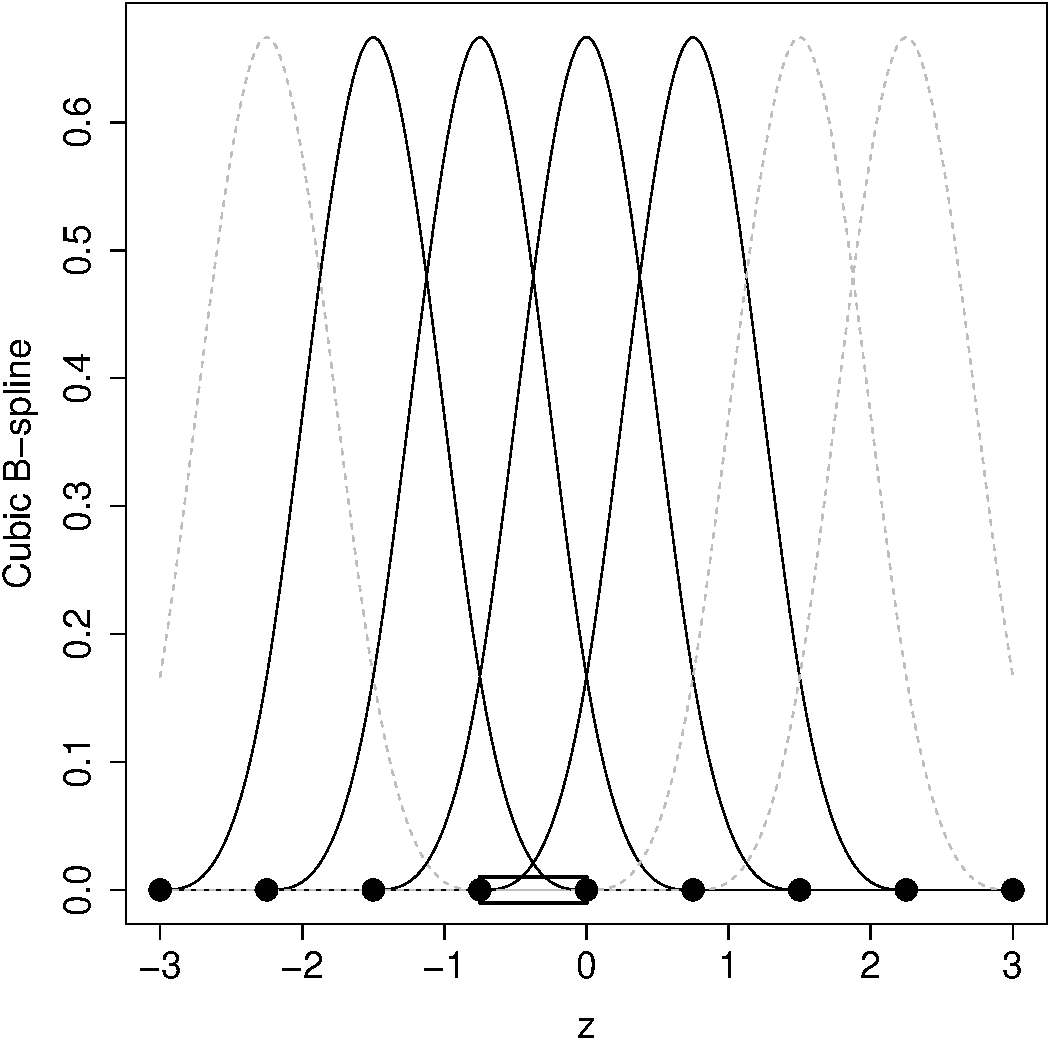
\includegraphics[width=0.48\textwidth, height=0.42\textwidth]{figs/bspline_cubic.pdf} &
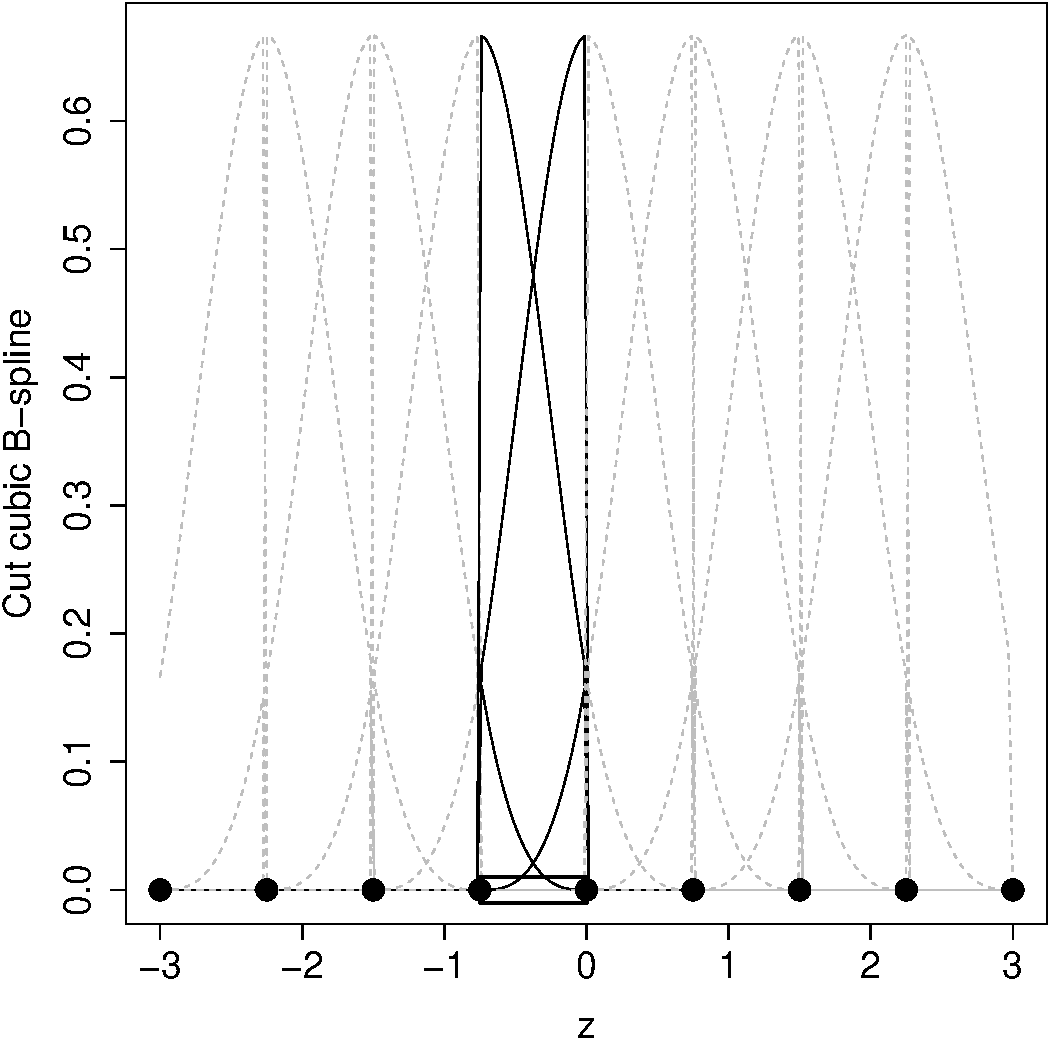
\includegraphics[width=0.48\textwidth, height=0.42\textwidth]{figs/cutspline_cubic.pdf} \\
\end{tabular}
\end{center}
\caption{Cubic B-splines (left) and cut cubic B-splines (right) for the simulated illustration in Figure \ref{fig:splinefit}.
%Top: true group means and their cubic B-spline projections (left), and posterior probability of local group differences for cubic and cut cubic B-splines based on $n=100$ (right).
%Bottom: basis functions for cubic (left) and the proposed cut cubic (right) splines, with corresponding knots and basis (right).
%{\color{red} M: the figure with the posterior probabilities of local group differences is not super clear}  
}
\label{fig:splinefit_suppl}
\end{figure}


\subsection{Extension of the example in Figure \ref{fig:splinefit}}

\begin{figure}
\begin{center}
\begin{tabular}{cc}
\multicolumn{2}{c}{12 knots for baseline, 8 knots for local tests} \\
$n=1000$ & $n=2000$ \\
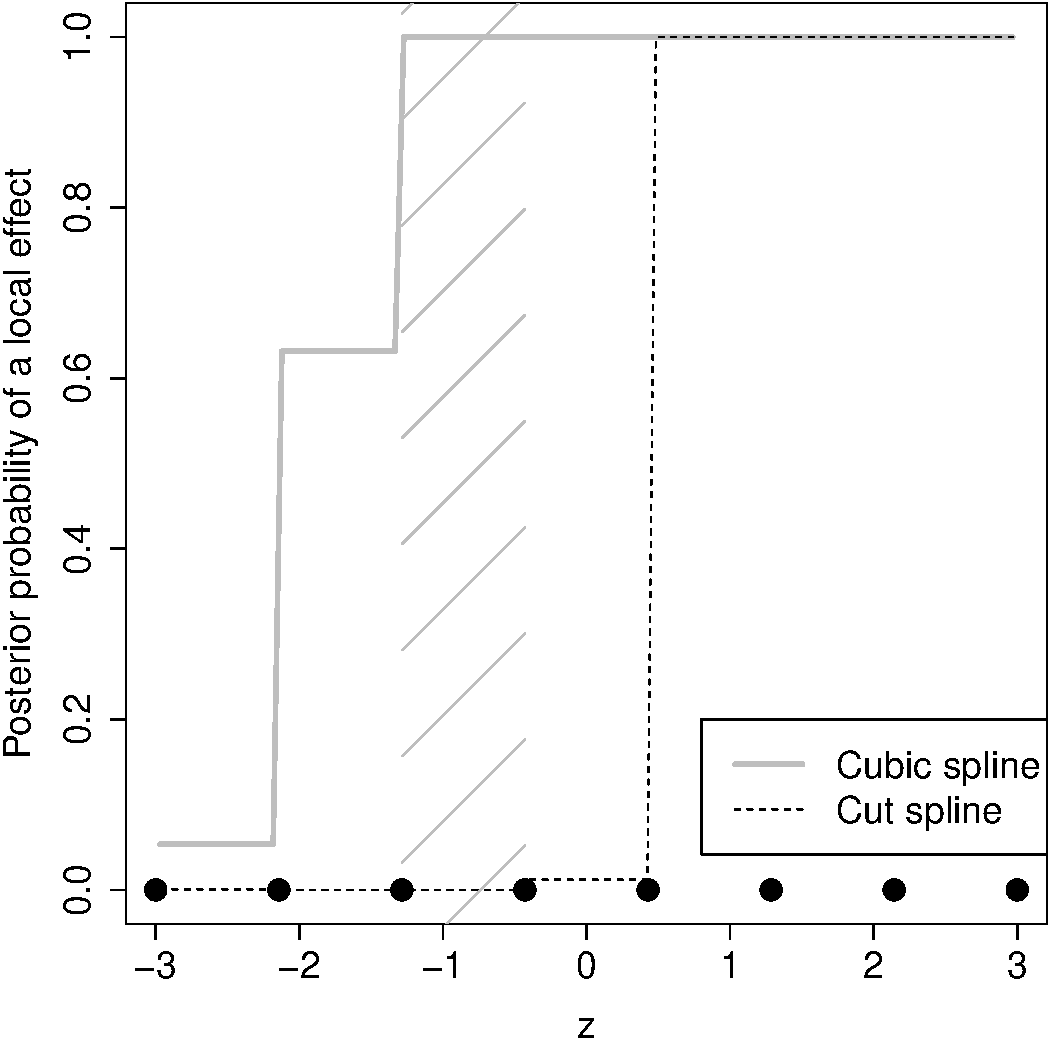
\includegraphics[width=0.48\textwidth, height=0.38\textwidth]{figs/bspline_cubic_pp_8knots.pdf} &
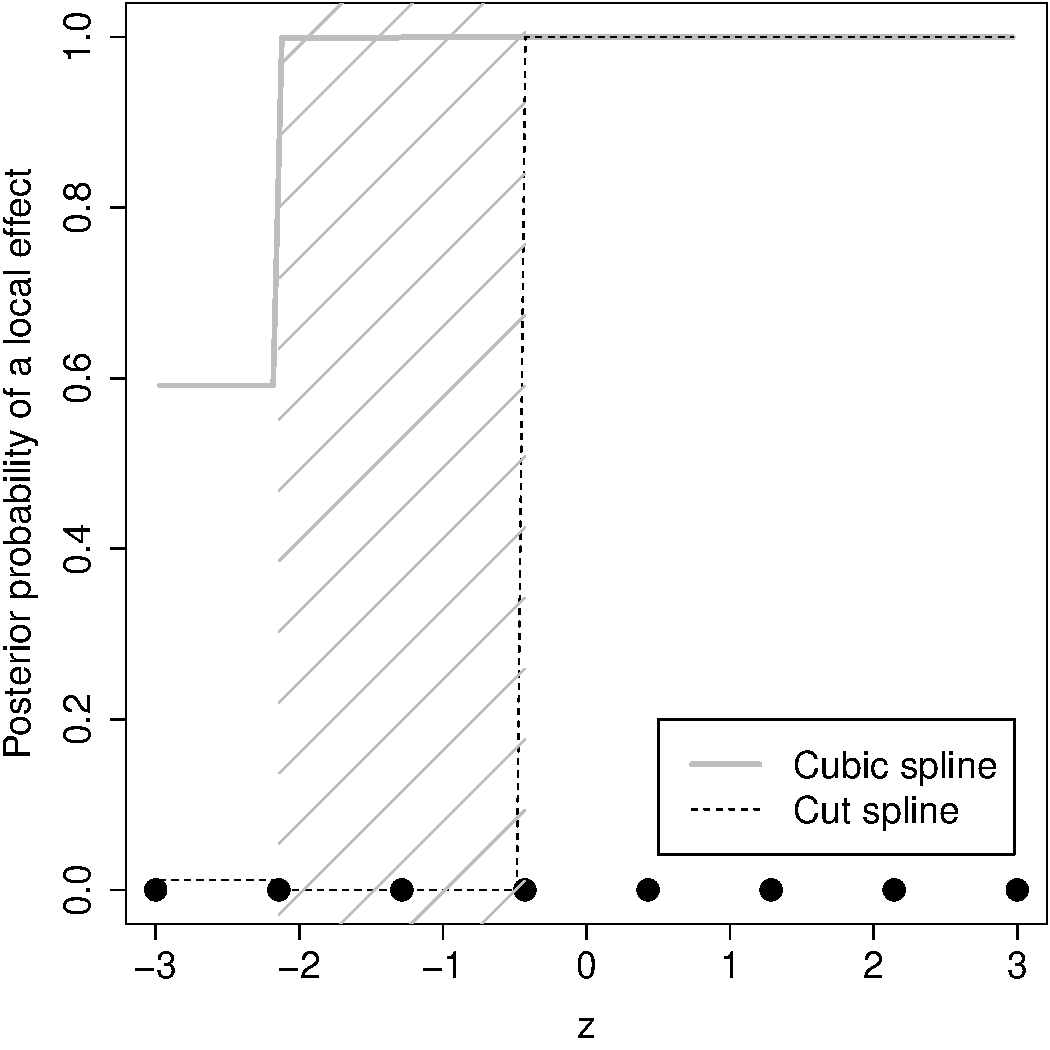
\includegraphics[width=0.48\textwidth, height=0.38\textwidth]{figs/bspline_cubic_pp_8knots_n2000.pdf} \\
\multicolumn{2}{c}{20 knots for baseline, 15 knots for local tests} \\
$n=1000$ & $n=2000$ \\
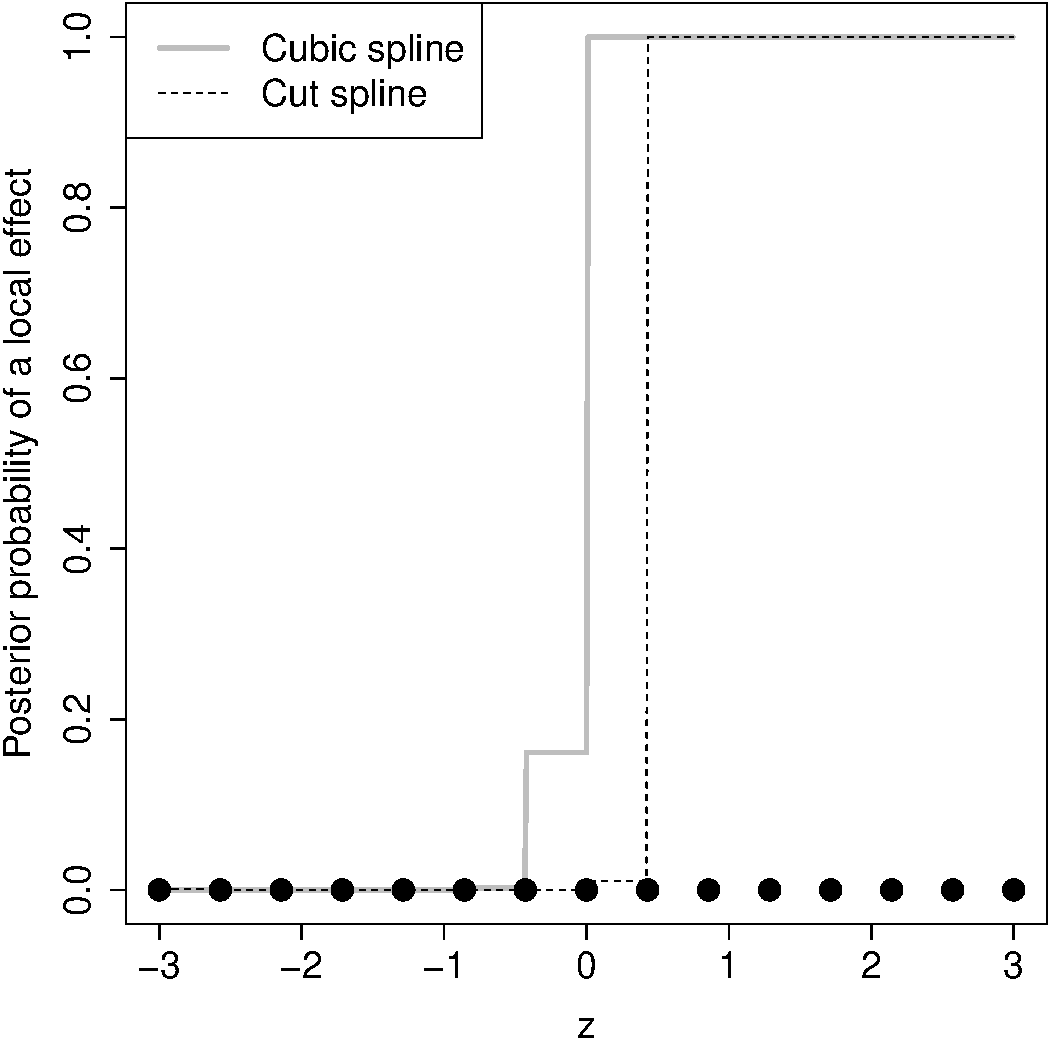
\includegraphics[width=0.48\textwidth, height=0.38\textwidth]{figs/bspline_cubic_pp_15knots.pdf} &
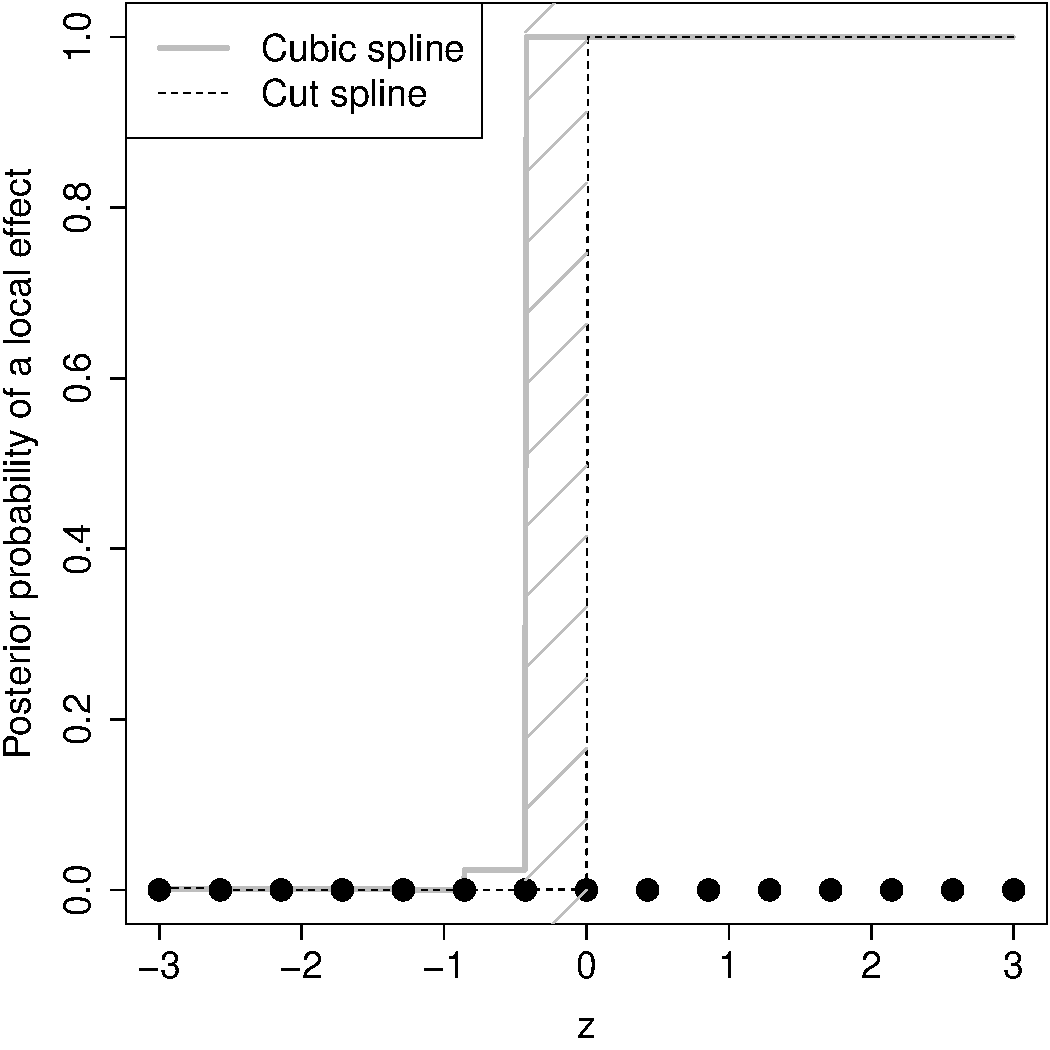
\includegraphics[width=0.48\textwidth, height=0.38\textwidth]{figs/bspline_cubic_pp_15knots_n2000.pdf} \\
\multicolumn{2}{c}{30 knots for baseline, 30 knots for local tests} \\
$n=1000$ & $n=2000$ \\
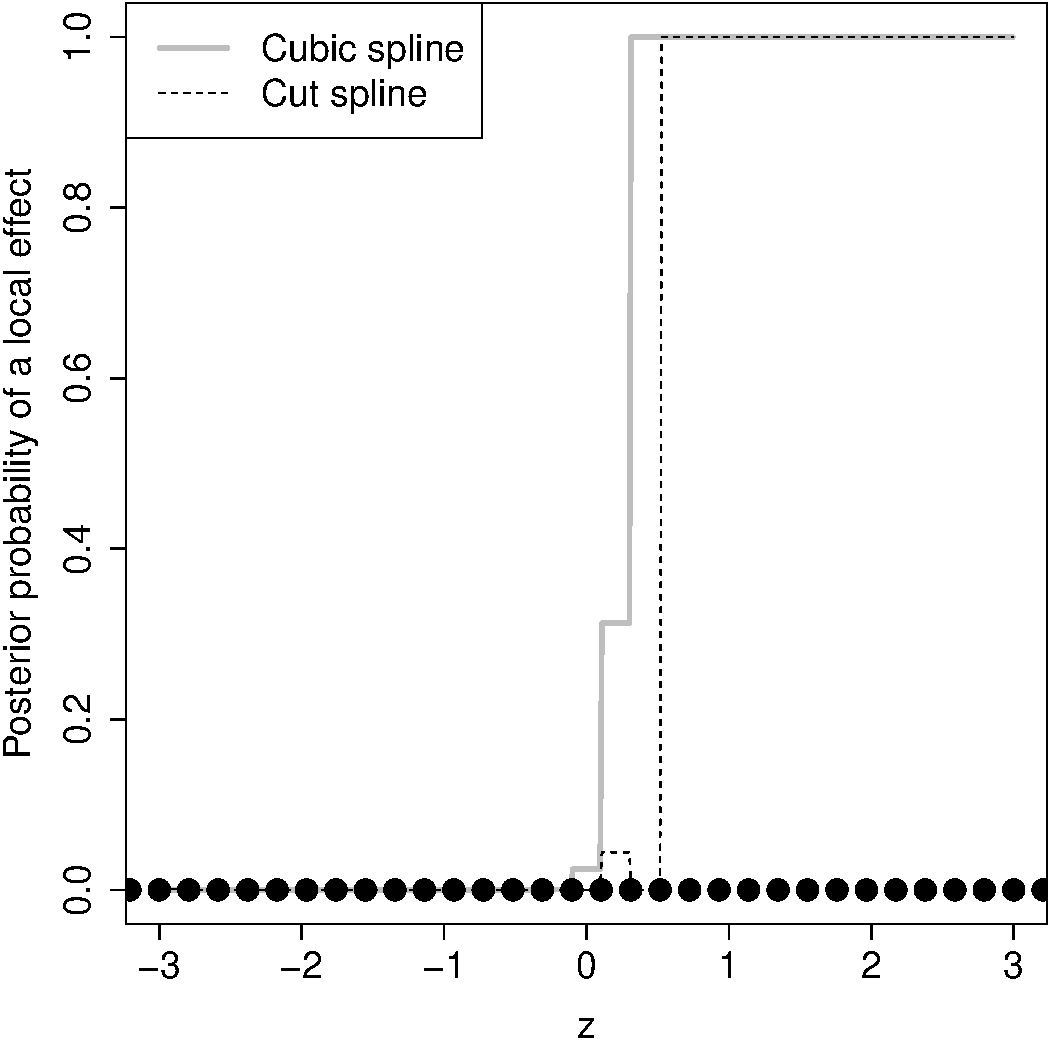
\includegraphics[width=0.48\textwidth, height=0.38\textwidth]{figs/bspline_cubic_pp_30knots.pdf} &
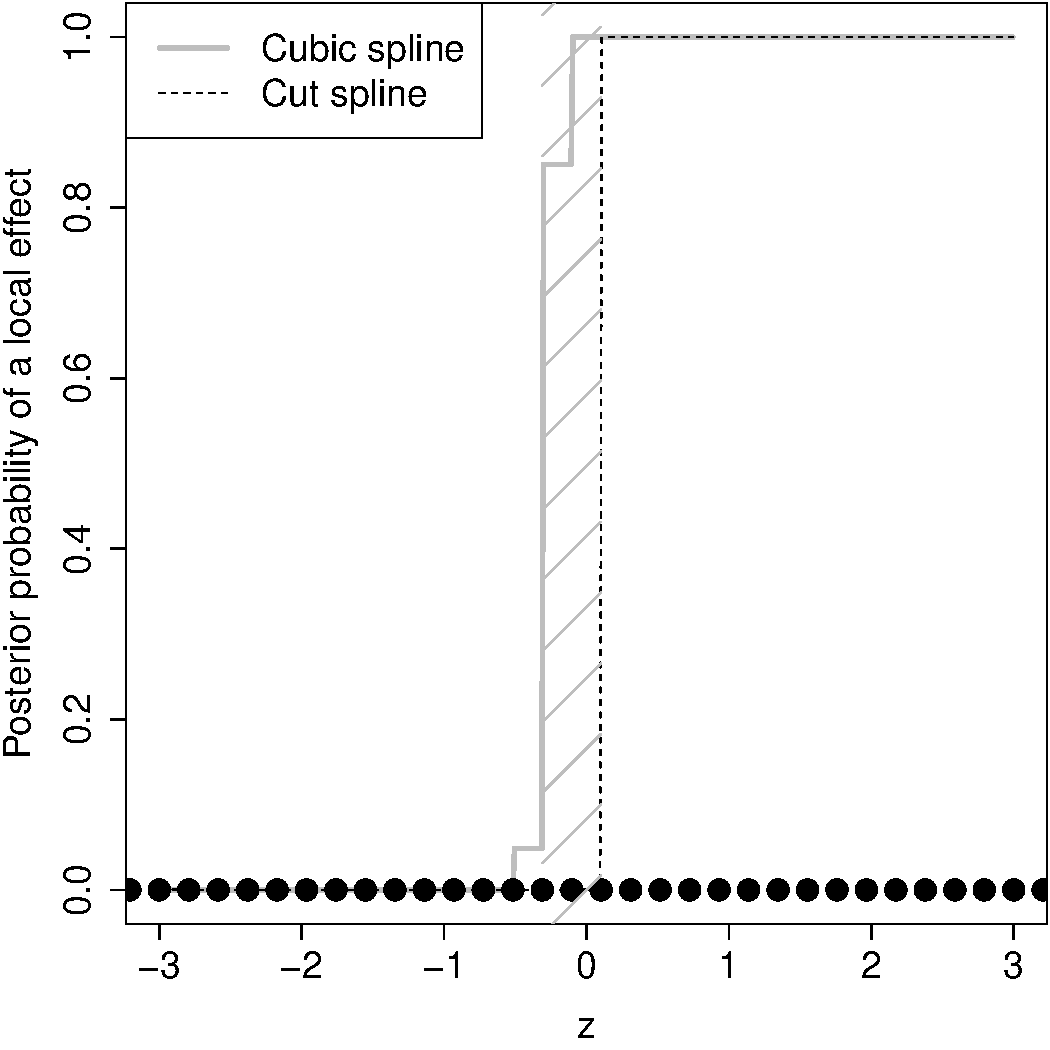
\includegraphics[width=0.48\textwidth, height=0.38\textwidth]{figs/bspline_cubic_pp_30knots_n2000.pdf} \\
\end{tabular}
\end{center}
\caption{Simulated illustration. Posterior probability of local group differences for cubic / cut cubic B-splines varying the knots and $n$. Shaded regions suffer from false positives}
\label{fig:splinefit_varyingknots}
\end{figure}


We extend the top panels in Figure \ref{fig:splinefit}, where one considers different number of knots and sample sizes.
Figure \ref{fig:splinefit_varyingknots} shows posterior probabilities for the presence of local group differences for the same examples as in Figure \ref{fig:splinefit}, but here we vary the number of knots and sample sizes.
The shaded areas indicate regions where there is false positive inflation, i.e. the posterior probability of a local covariate effect in that region is large, but there's truly no effect.
Overall the same phenomenon persists, for larger $n$ the standard B-splines leads to falsely rejecting the null in a neighborhood of $z<0$, whereas the cut B-splines avoid the false positive issue. 
The bottom left panel illustrates how, if the number of knots is too large, the power to detect local differences decreases, in this case for $z \in [0,0.5]$.




\subsection{Simulation with independent errors}
\label{ssec:simulation_iid}

We outline supplementary results for the simulation study presented in Section \ref{sec:simulation_iid} of the main manuscript.
%Table \ref{tab:simiid} shows type I error and power (across 100 simulations) for the various considered methods.
Figure \ref{fig:simiid} shows the posterior probability (average across 100 simulations) for the presence of a covariate effect as a function of $z$.
Covariate 1 is truly active for $z>0$ and inactive for $z \leq 0$, covariates 2-10 are truly inactive at any $z \in [-3,3]$.


Table \ref{tab:simiid_extra} provide further results regarding our simulation with independent errors, related to using alternative methods to those described in the main paper.
It shows the average proportion of rejected local null hypotheses, separately for covariate 1 (which is truly active for $z>0$) and the other covariates.
Specifically, it considers a Benjamini-Hochberg P-value adjustment from a least-squares fit, a fused LASSO fit based on our degree 0 cut orthogonal basis, standard (uncut) cubic splines (which, as opposed to our cut orthogonal splines, runs into false positive issues) and a generalized additive model in mgcv with twice the default knots (24 knots).
%For our methodology, we show the results from using either a Gaussian shrinkage prior on the coefficients (diagonal covariance) or an ICAR+ prior. Local null hypotheses are rejected when $P(\beta_j(z) \neq 0 \mid y) > 0.95$.
%We also considered VC-BART, generalized additive models from R package mgcv (with the default 12 knots and also with 24 knots), applying the fused LASSO to our cut orthogonal basis, and applying Benjamini-Hochberg P-value adjustment.

%The results for the Gaussian shrinkage and ICAR+ priors were very similar. Both controlled the type I error below the 0.01 level, and exhibited a high power to detect truly non-zero local effects ($\beta_1(z) \neq 0$, for $z>0$).
%VC-BART and the additive model showed a competitive performance, albeit the type I error was above 0.05 in several instances.
Benjamini-Hochberg adjusted P-values were too conservative, exhibiting very low power for $n=100$, whereas the fused LASSO was overly liberal, with type I errors that were above 0.1 even when $n=1000$.
The uncut cubic splines and GAM resulted in an inflated type I error for covariate 1, for $z \in (0,1]$.


Table \ref{tab:simiid_mse} displays the root mean squared error for the various considered methods.


\begin{table}
\begin{center}
\begin{tabular}{ccccccccc} %\hline
\multicolumn{9}{c}{$n=100$} \\ %\hline
& \multicolumn{4}{c}{Covariate 1} & \multicolumn{4}{c}{Covariates 2-10} \\ %\hline
 Region          & BH  &  Fused       & Cubic       & GAM          & BH    &  Fused        & Cubic & GAM \\ 
                 &     &  LASSO       & uncut       & 24 knots   &       &  LASSO        & uncut & 24 knots \\ 
$z \in $ (-3,-2] & 0   &  0.69$^{**}$ &     0        &  0.04        & 0     &  0.35 $^{**}$ & 0     &  0.04 \\ 
$z \in $ (-2,-1] & 0   &  0.89$^{**}$ &     0        &  0.03        & 0     &  0.52 $^{**}$ & 0     &  0.04 \\ 
$z \in $  (-1,0] & 0   &  0.82$^{**}$ &     1$^{**}$ &  0.28$^{**}$  & 0     &  0.56$^{**}$  &  0     &  0.05 \\ 
$z \in $   (0,1] & 0.01&  0.91$^{**}$ &     1        &  0.79        & 0.004 &  0.50 $^{**}$ & 0     &   0.05\\ 
$z \in $   (1,2] & 0   &  0.89$^{**}$ &     1        &  0.99        & 0     &  0.21 $^{**}$ & 0     &   0.05\\ 
$z \in $   (2,3] & 0   &  0.95$^{**}$ &     1        &  0.94        & 0     &  0.52 $^{**}$ & 0     &  0.04 \\ 
%\hline
\multicolumn{9}{c}{$n=1000$} \\ %\hline
& \multicolumn{4}{c}{Covariate 1} & \multicolumn{4}{c}{Covariates 2-10} \\ %\hline
 Region         & BH   & Fused        & Cubic  & GAM         & BH    &  Fused & Cubic    & GAM  \\ 
                &     &  LASSO        & uncut  & 24 knots  &       &  LASSO & uncut    & 24 knots \\ 
$z \in $(-3,-2] & 0    &  0.22$^{**}$ & 0       &  0.0008     & 0.004 &  0.07 & 0          & 0.006  \\ 
$z \in $(-2,-1] & 0    &  0.13$^{**}$ & 0.01    &  0.0002     & 0.004 &  0    & 0          & 0.006  \\ 
$z \in $ (-1,0] & 0    &  0.12$^{**}$ & 1$^{**}$ &  0.08$^{**}$& 0    &   0.06 &  0          & 0.01  \\ 
$z \in $  (0,1] & 1    &  1          & 1       &  0.95       & 0.006 &  0    & 0          & 0.01 \\ 
$z \in $  (1,2] & 0.515&  1          & 1       &  1          & 0.001 &  0.05 & 0          & 0.01   \\ 
$z \in $  (2,3] & 1    &  1          & 1       &  1          & 0.002 &  0    & 0          & 0.01  \\ 
%\hline
\end{tabular}
\end{center}
\caption{Independent errors simulation. Proportion of rejected null hypothesis for several methods.
For covariate 1 and $z>0$,  this proportion is the statistical power; otherwise, it is the type I error. ** indicates a type I error $> 0.05$.
The methods are applying Benjamini-Hochberg P-value adjustment
and fused LASSO to our degree 0 cut splines,
using uncut cubic splines in our Bayesian framework, and a GAM with 24 knots.
For fused LASSO the tuning parameters are set to minimize the extended Bayesian information criterion, further only estimates above 0.1 in absolute value are reported as significant}
\label{tab:simiid_extra}
\end{table}


\begin{figure}
\begin{center}
\begin{tabular}{cc}
Average $P(\beta_j(z) \neq 0 \mid y)$ & Proportion of rejected null hypotheses \\
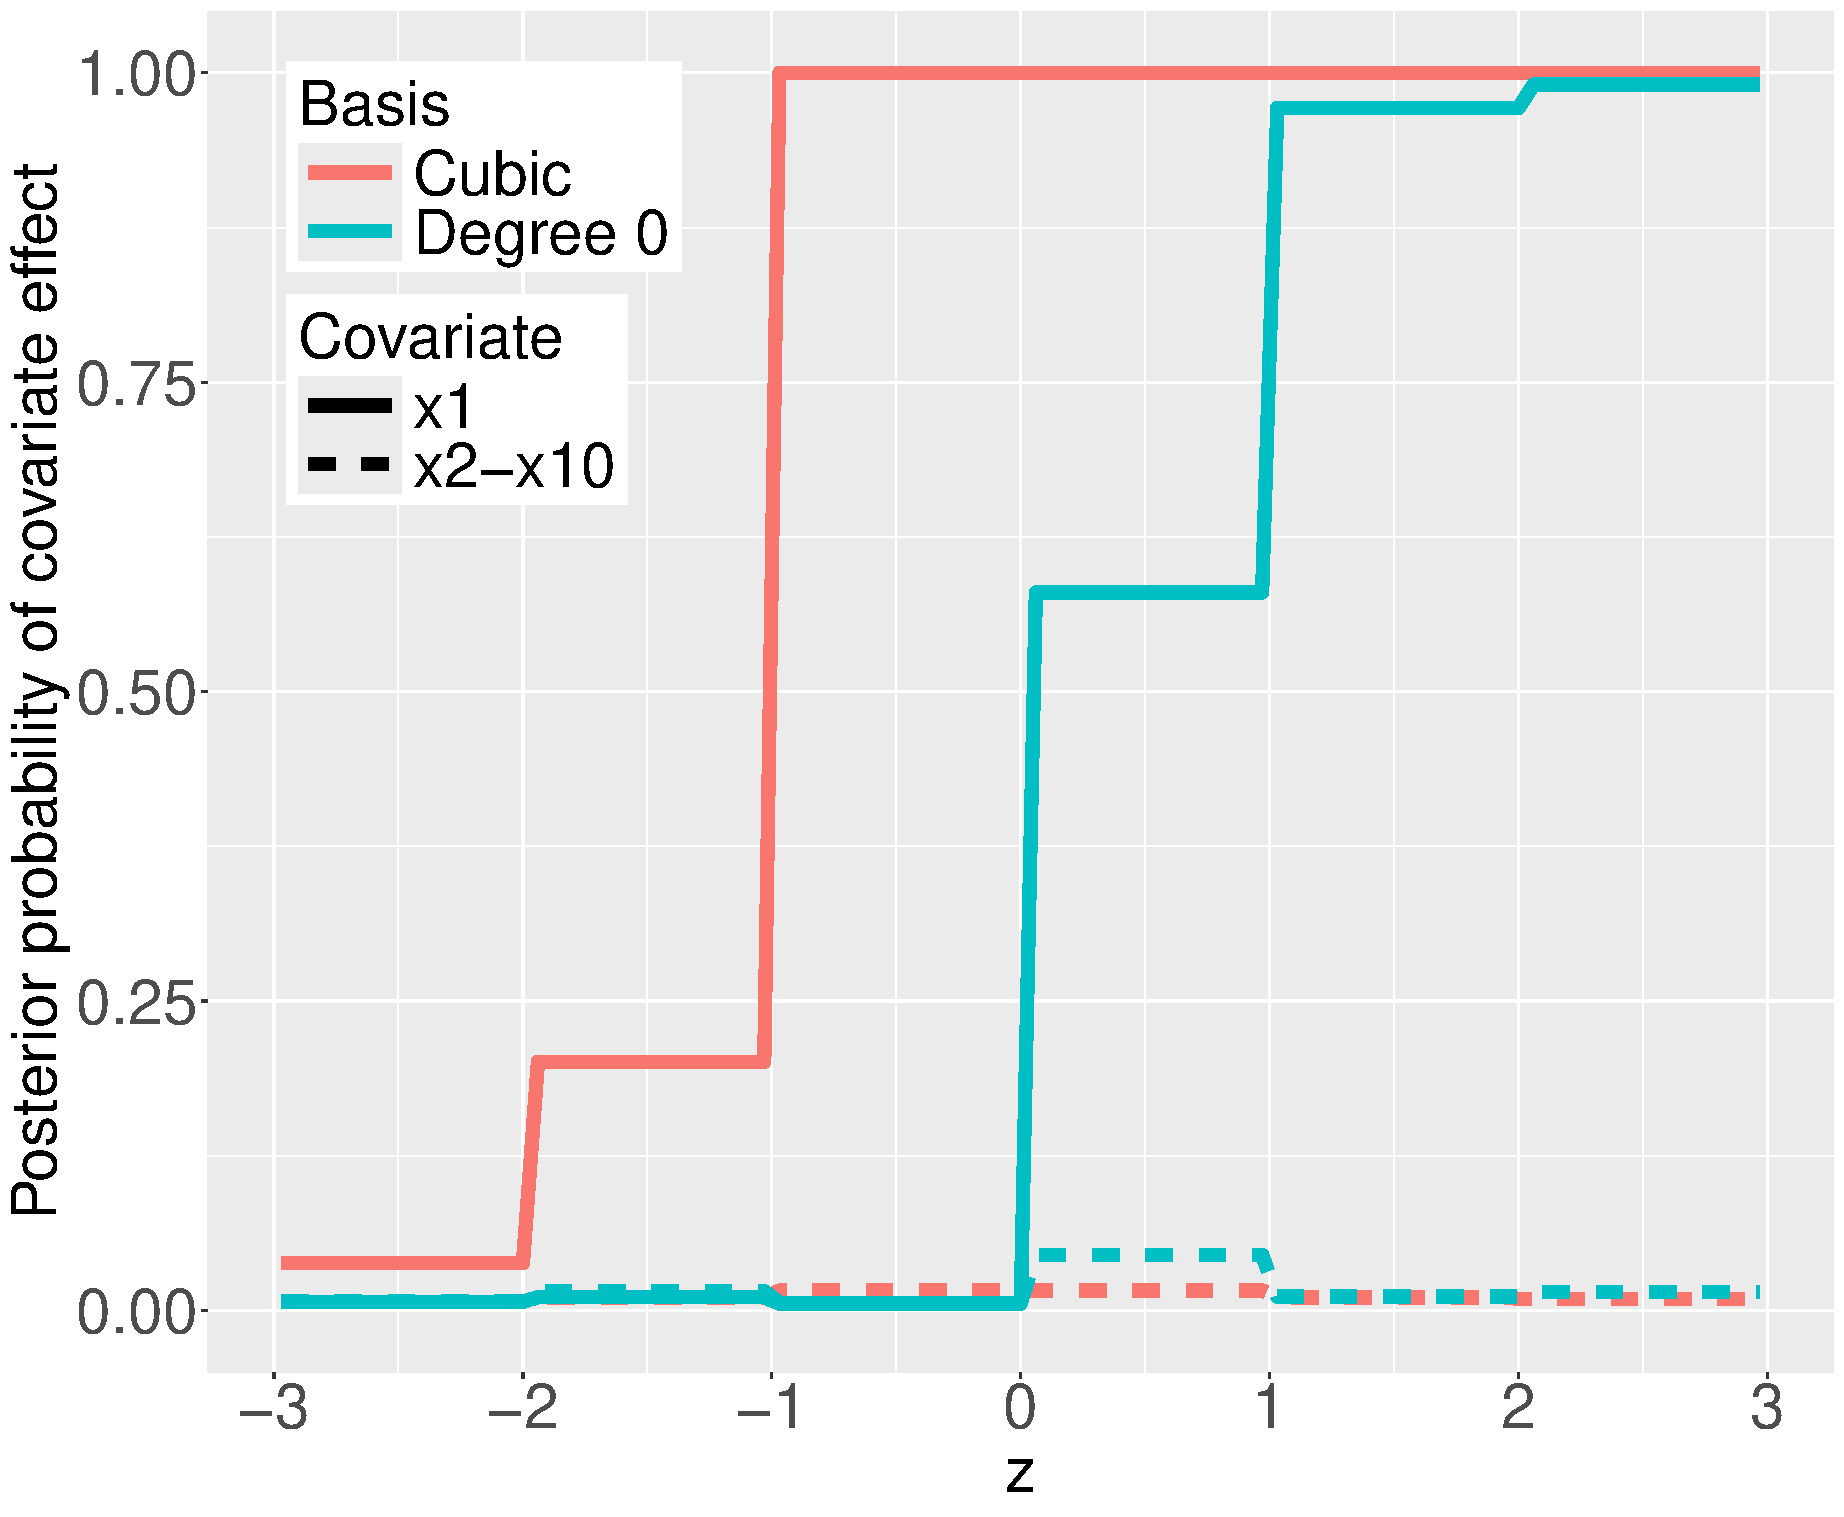
\includegraphics[width=0.5\textwidth]{figs/simiid_pp_n100.pdf} &
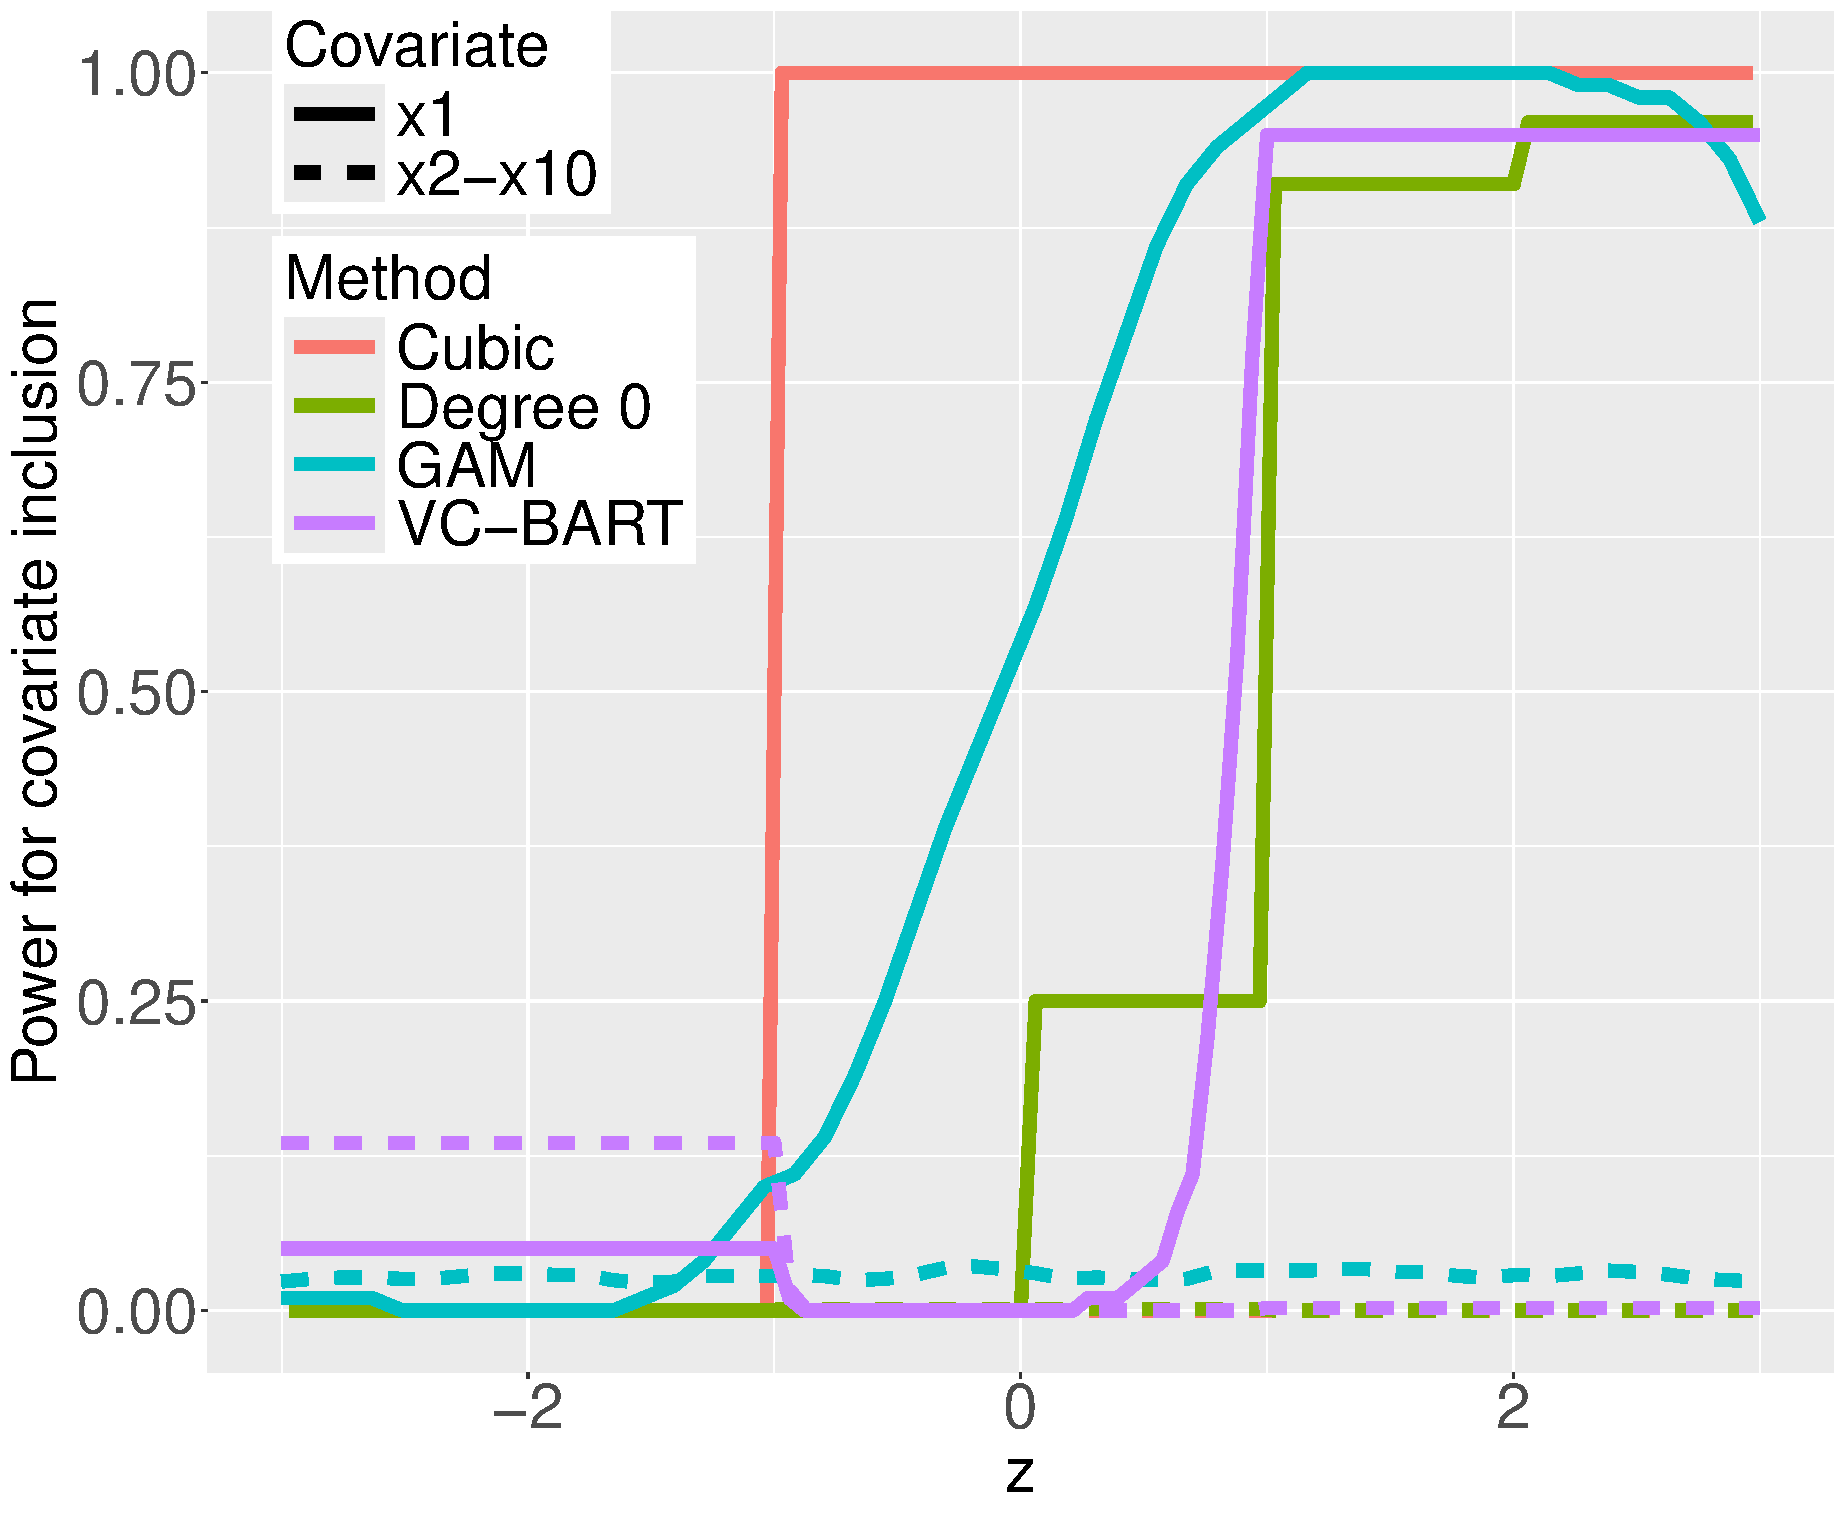
\includegraphics[width=0.5\textwidth]{figs/simiid_pow_n100.pdf} \\
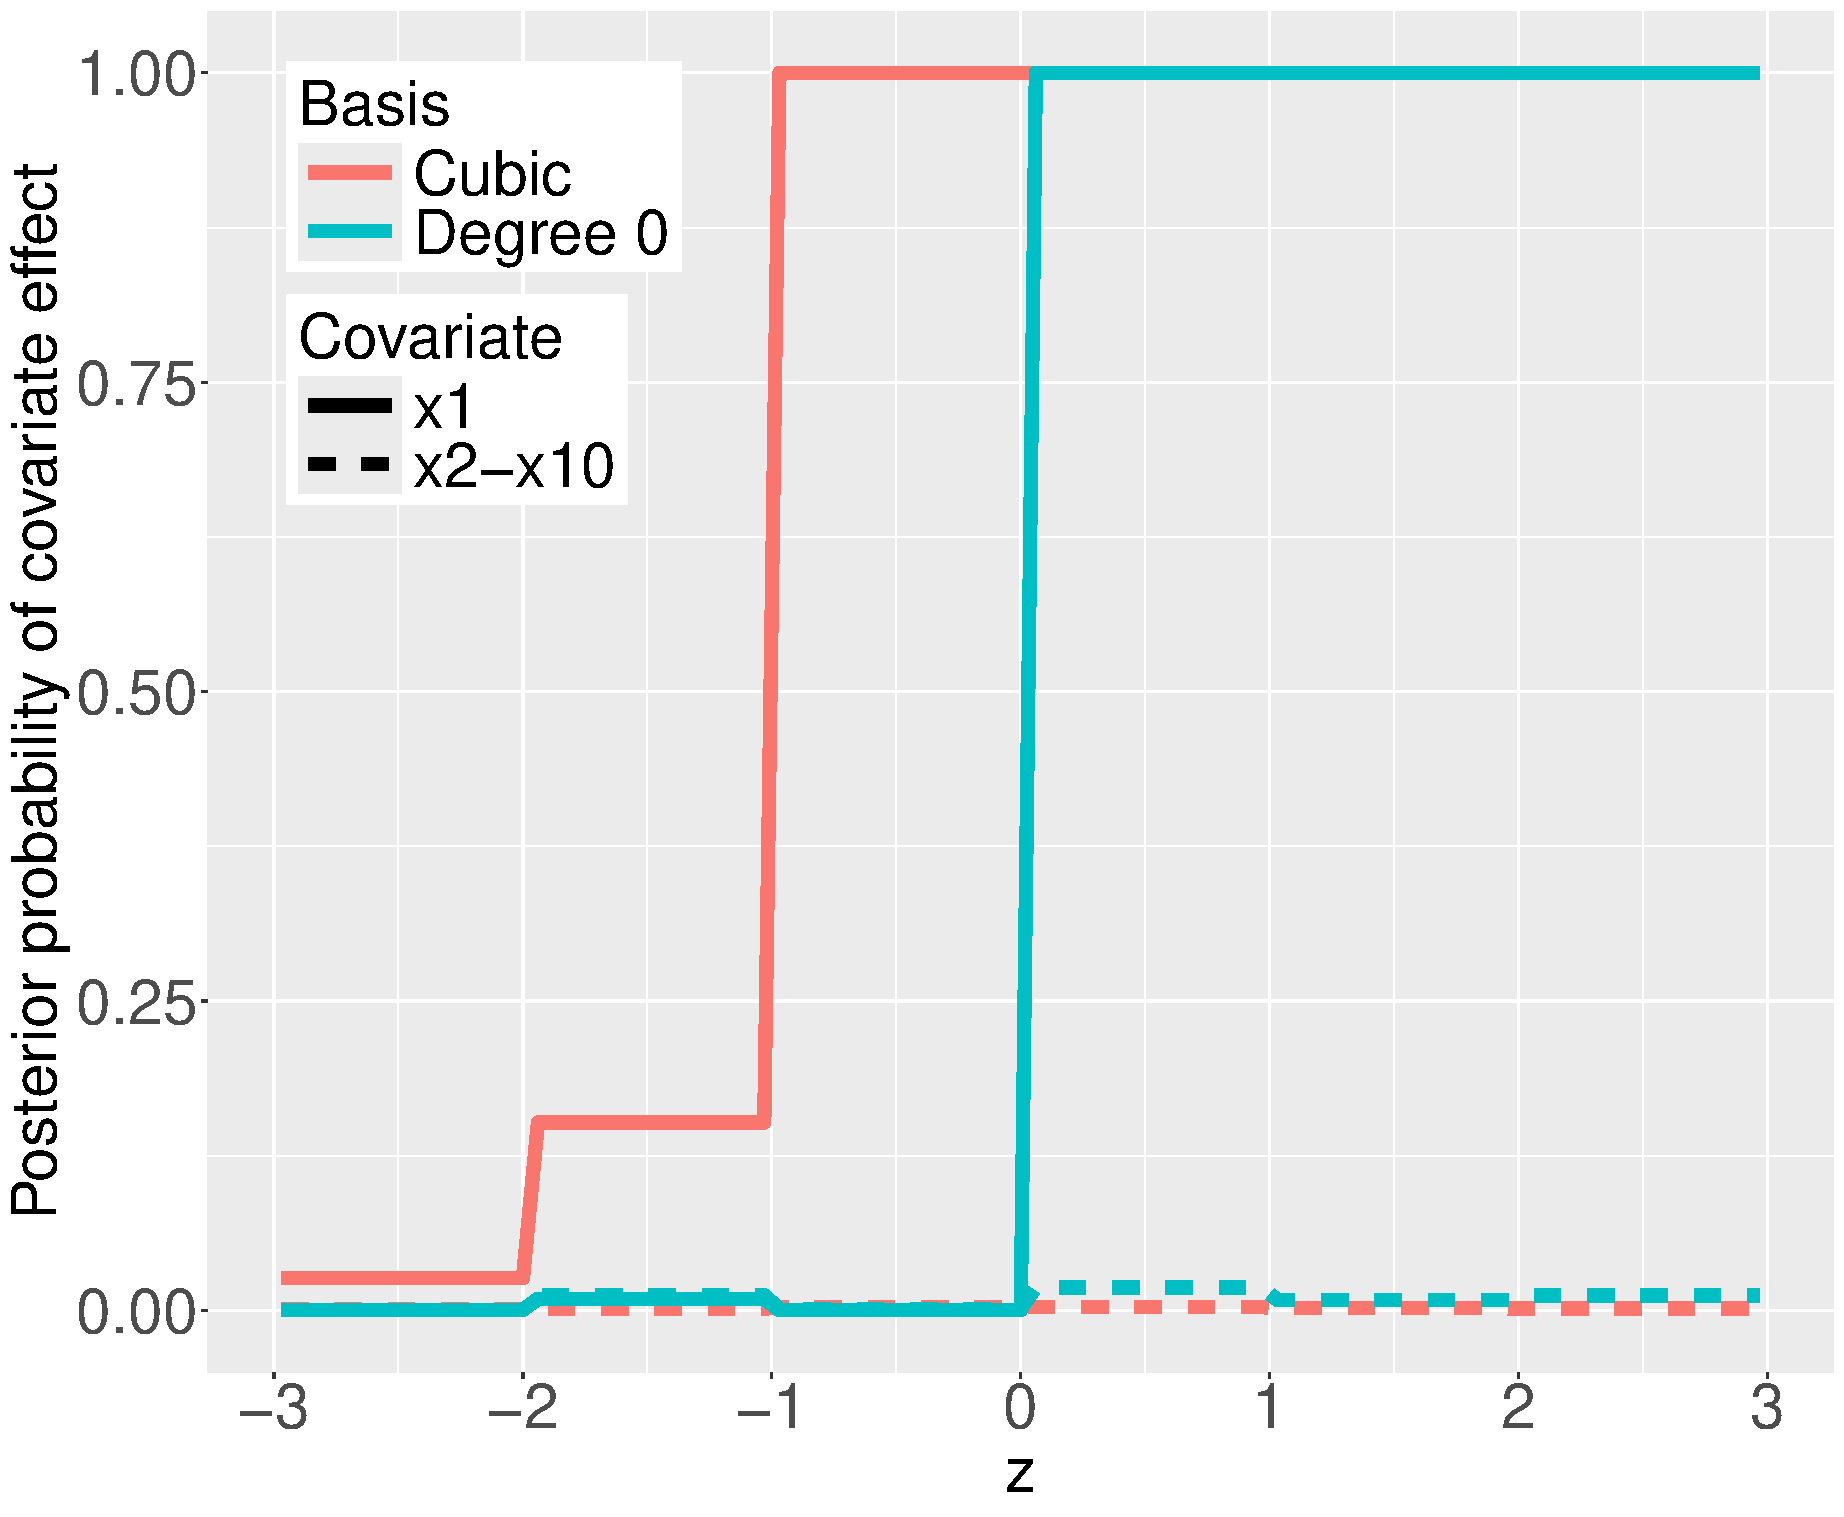
\includegraphics[width=0.5\textwidth]{figs/simiid_pp_n1000.pdf} &
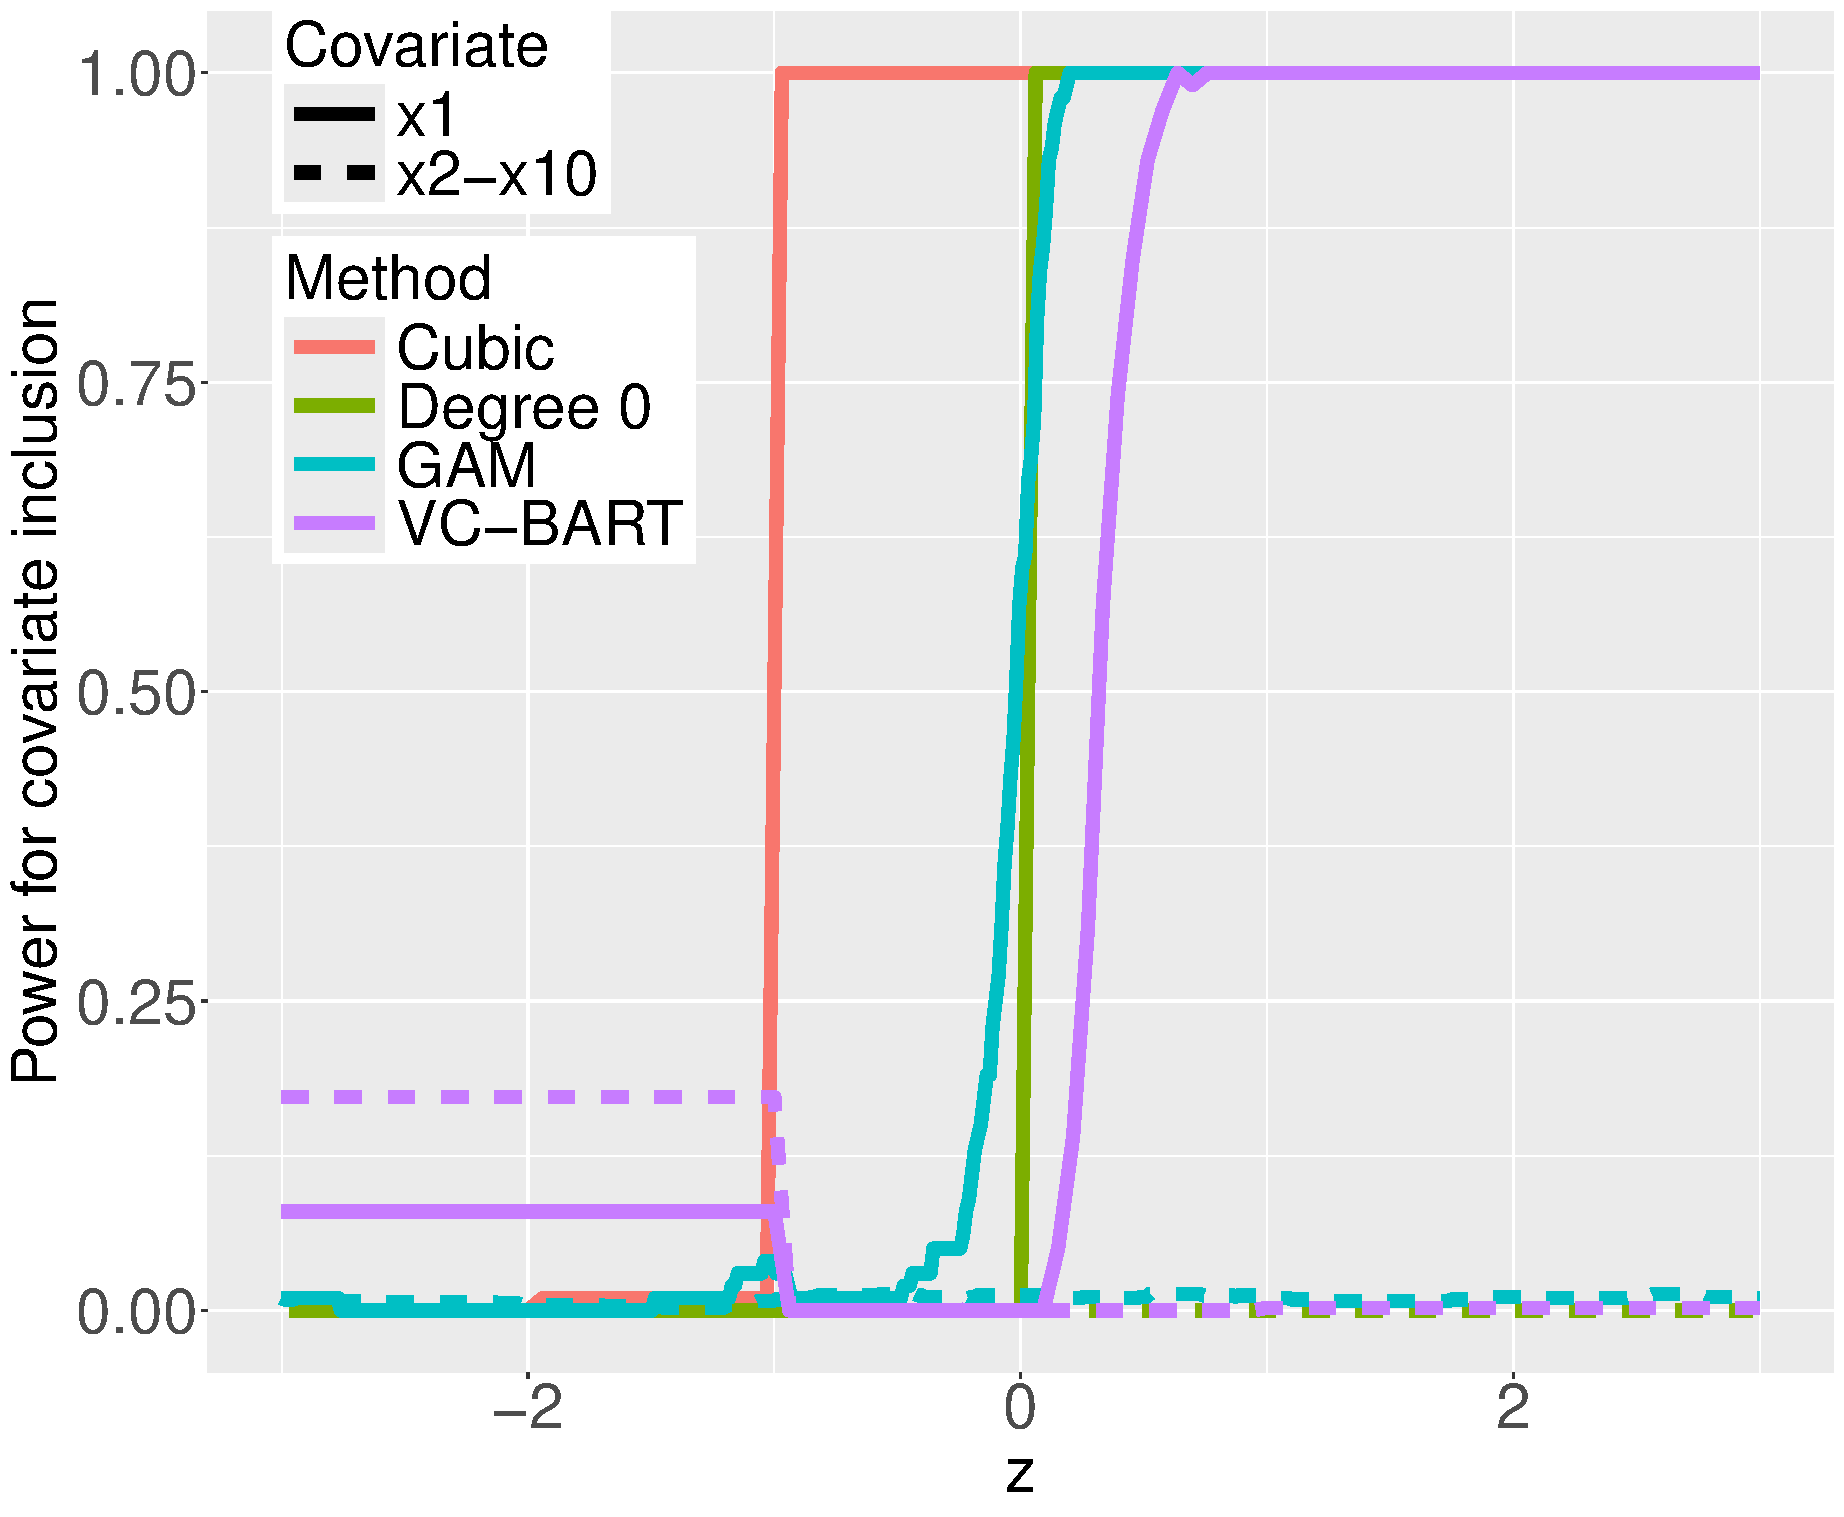
\includegraphics[width=0.5\textwidth]{figs/simiid_pow_n1000.pdf}
\end{tabular}
\end{center}
\caption{Independent errors simulation. Posterior probability of local null test and proportion of rejected null hypotheses. Top: $n=100$. Bottom: $n=1,000$}
\label{fig:simiid}
\end{figure}


\begin{table}
\begin{center}
\begin{tabular}{lcccccc}  %\hline
         & Gaussian &  ICAR+ & Cubic    & VC-BART & GAM        & GAM \\ 
         & prior    &  prior & B-splines&         & 12 knots & 24 knots\\   %\hline
n=100    & 0.173    &  0.166 & 0.168    & 0.297   & 0.159      & 0.173  \\ 
n=1000   & 0.063    &  0.063 & 0.078    & 0.285   & 0.055      & 0.058 \\ 
   %\hline
\end{tabular}
\end{center}
\caption{Independent errors simulation. Root Mean Squared Error $E_F\left[ \hat{E}(y_i) - E_F(y_i) \right]^2$ for 0-degree cut splines, cubic B-splines, VC-BART  and GAM (R package mgcv) with $k=12$ and $k=24$ knots }
\label{tab:simiid_mse}
\end{table}


\begin{table}
\begin{center}
\begin{tabular}{ccc} %\hline
                                                 & $n=100$  & $n=1,000$ \\ %\hline
%David's desktop. NEW mombf version
Gaussian shrinkage prior. Cut degree 0 (1 core)  &   8.5 sec &  5.5 sec  \\ 
Gaussian shrinkage prior. Cut degree 0 (3 cores) &   5.0 sec &  4.0 sec  \\ 
ICAR+ prior. Cut degree 0 (1 core)               &   53.3 sec &  20.3 sec  \\ 
ICAR+ prior. Cut degree 0 (3 cores)              &   31.4 sec &  12.3 sec  \\ 
%David's laptop. NEW mombf version
%Normal shrinkage. Cut degree 0 (1 core)  &  14.9 sec& 9.6 sec \\ 
%Normal shrinkage. Cut degree 0 (3 cores) &   8.8 sec& 7.1 sec \\ 
%ICAR+ prior. Cut degree 0 (1 core)               &   95.1 sec &  36.3 sec  \\ 
%ICAR+ prior. Cut degree 0 (3 cores)              &   56.0 sec &  21.9 sec  \\ 
VCBART          &  69.2 sec  & 7.05 min \\
GAM ($k=12$)             &  1.4 sec  & 4.2 sec\\
GAM ($k=24$)             &  1.3 sec  & 4.2 sec\\
%David's desktop. PREVIOUS mombf version (no fast Cholesky updates)
%Cut degree 0 (1 core)  &  33.6 sec & 27.6sec \\ 
%Cut degree 0 (3 cores) &  22.0 sec& 21.8 sec \\ 
%David's laptop. PREVIOUS mombf version
%Cut degree 0 (1 core)  &  58.2sec & 59.1sec \\ 
%Cut degree 0 (3 cores) &  39.1 sec& 40.8sec \\ 
%VCBART          &  2.2min  & 12.6min \\ 
%\hline
\end{tabular}
\end{center}
\caption{Independent errors simulation. Run times for one simulation on an Ubuntu Linux desktop, 13th Gen Intel core i7 processor, 32Gb RAM}
\label{tab:cputime_simiid}
\end{table}




\subsection{Simulation with independent errors, misaligned knots}
\label{ssec:simulation_iid_misalign}

We extend the simulation results in Section \ref{ssec:simulation_iid} by considering a variation where all the knots in our methodology are misaligned with respect to the true changepoint where $\beta_1(z)$ transitions from zero to non-zero.
Specifically, all settings are equal to those of Section \ref{ssec:simulation_iid}, except that now we set a data-generating $\beta_1(z) = 0$ for $z \leq 0.15$ and $\beta_1(z) \neq 0$ for $z > 0.15$. Recall that $\beta_1(z)$ is the coefficient associated to a binary covariate, hence it defines two group means.
The top panel in Figure \ref{fig:simiid_unaligned} shows this data-generating means for both groups, along with the knots used in our multi-resolution analysis (using our default of 3 resolutions, 
The middle and bottom panels show the average posterior probability $P(\beta_j(z) \neq 0 \mid y)$ and the proportion of rejected local null hypotheses (using a cutoff of $P(\beta_j(z) \neq 0 \mid y) > 0.95$) as a function of $z$.

The results are very similar to those in Section \ref{ssec:simulation_iid}, with some nuisances.
First, note that our specified knots define regions that start at $z=0$ and include the true changepoint $z=0.15$, i.e. regions where $\beta_j(z) \neq 0$ for some $z$ in the region.
Therefore, our approach finds evidence for the existence differences are found within such a region.
That is, our posterior probabilities should be interpreted as there being evidence for differences somewhere in the region.

A second observation is that the average posterior probability and power for $z \in [0,1]$ are slightly lower than in Section \ref{ssec:simulation_iid}, where the knots for two resolutions were aligned with the true changepoint. Intuitively, since truly $\beta_j(z)=0$ for some $z$'s in the region, the statistical power decreases relative to a perfectly aligned region where $\beta_j(z) \neq 0$ for all $z$ in that region.


\begin{figure}
\begin{center}
\begin{tabular}{c}
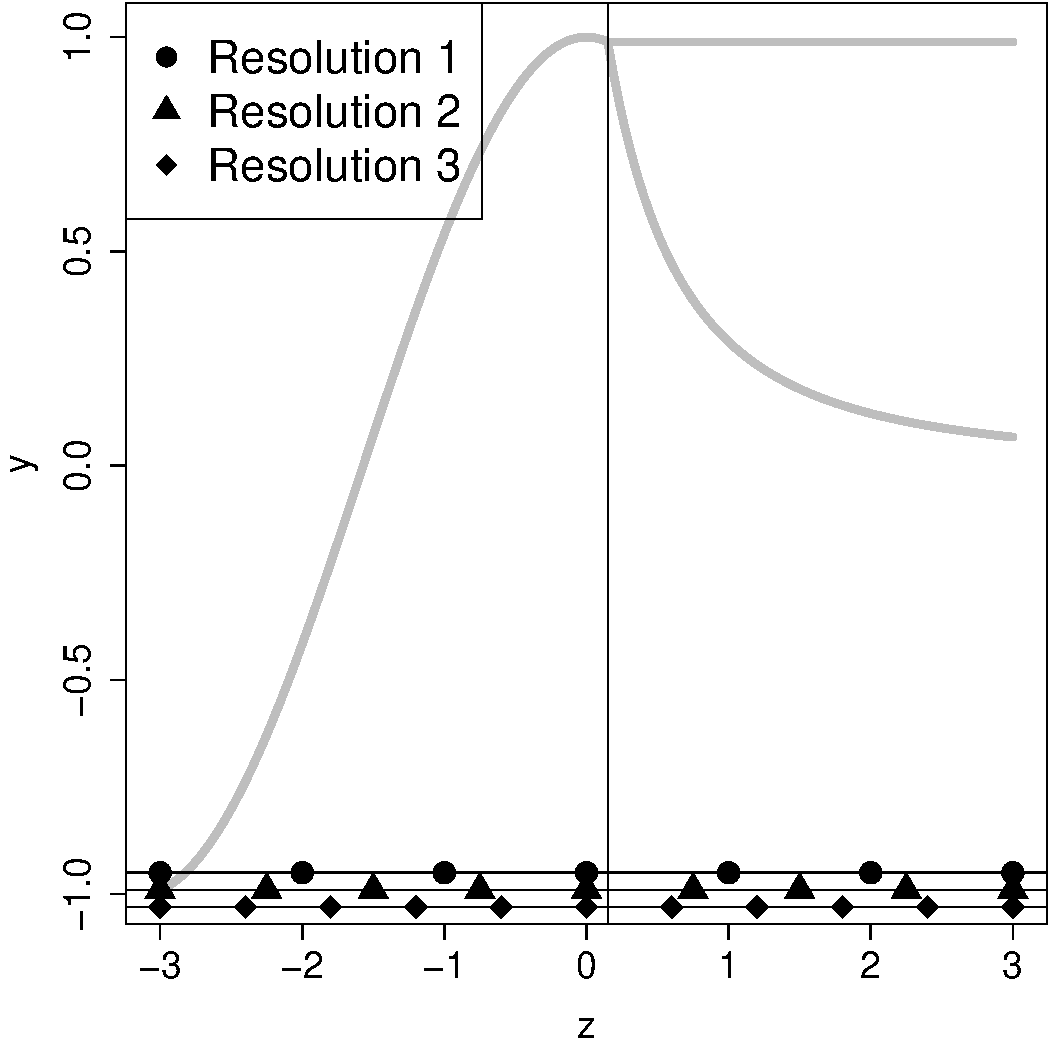
\includegraphics[width=0.5\textwidth,height=0.4\textwidth]{figs/simiid_unaligned.pdf} \\
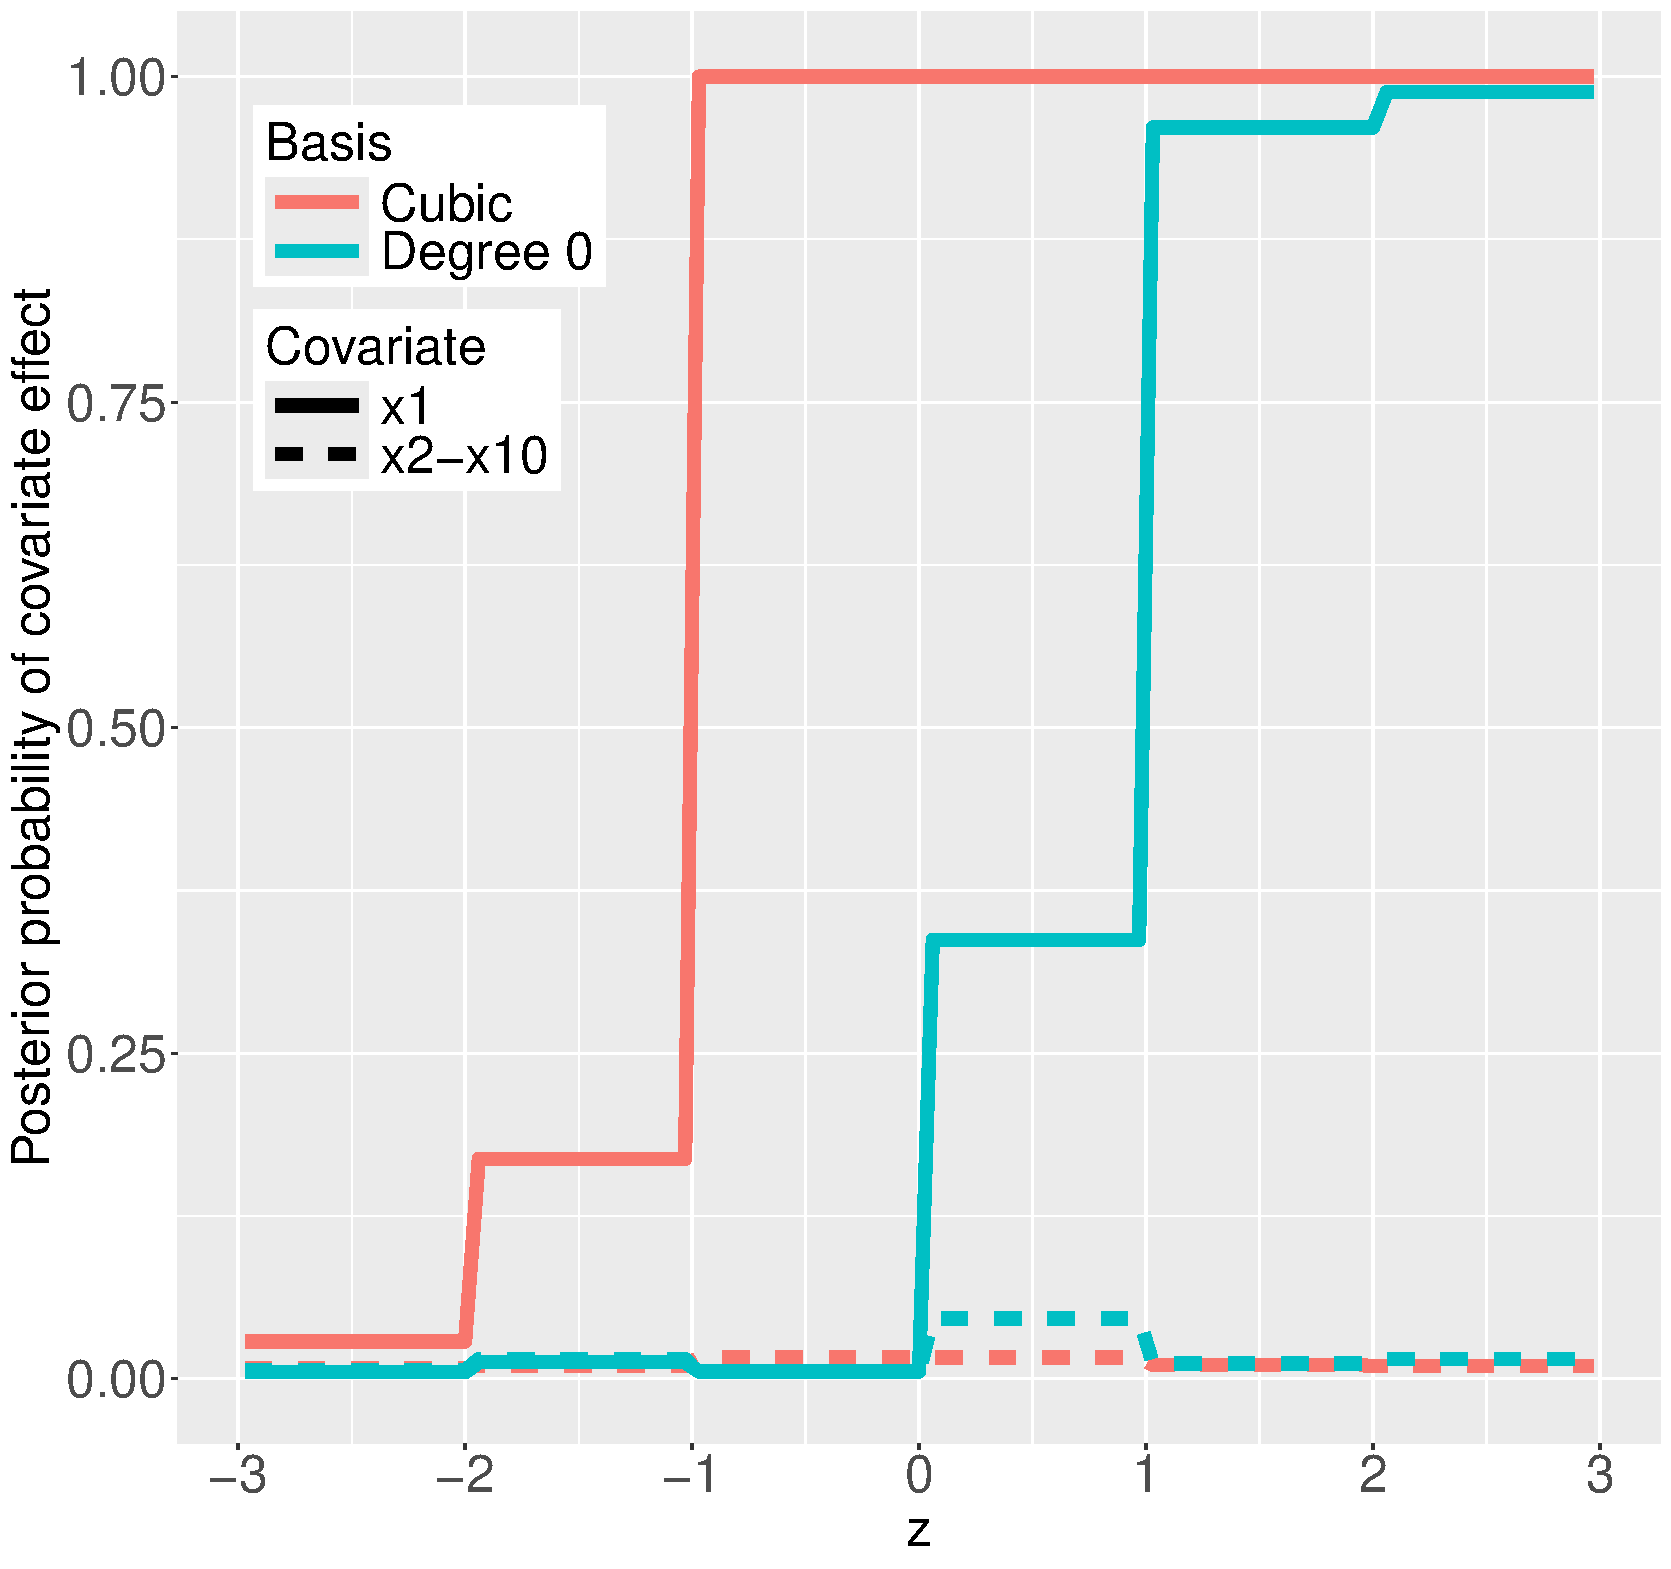
\includegraphics[width=0.5\textwidth,height=0.4\textwidth]{figs/simiid_unaligned_pp_n100.pdf} \\
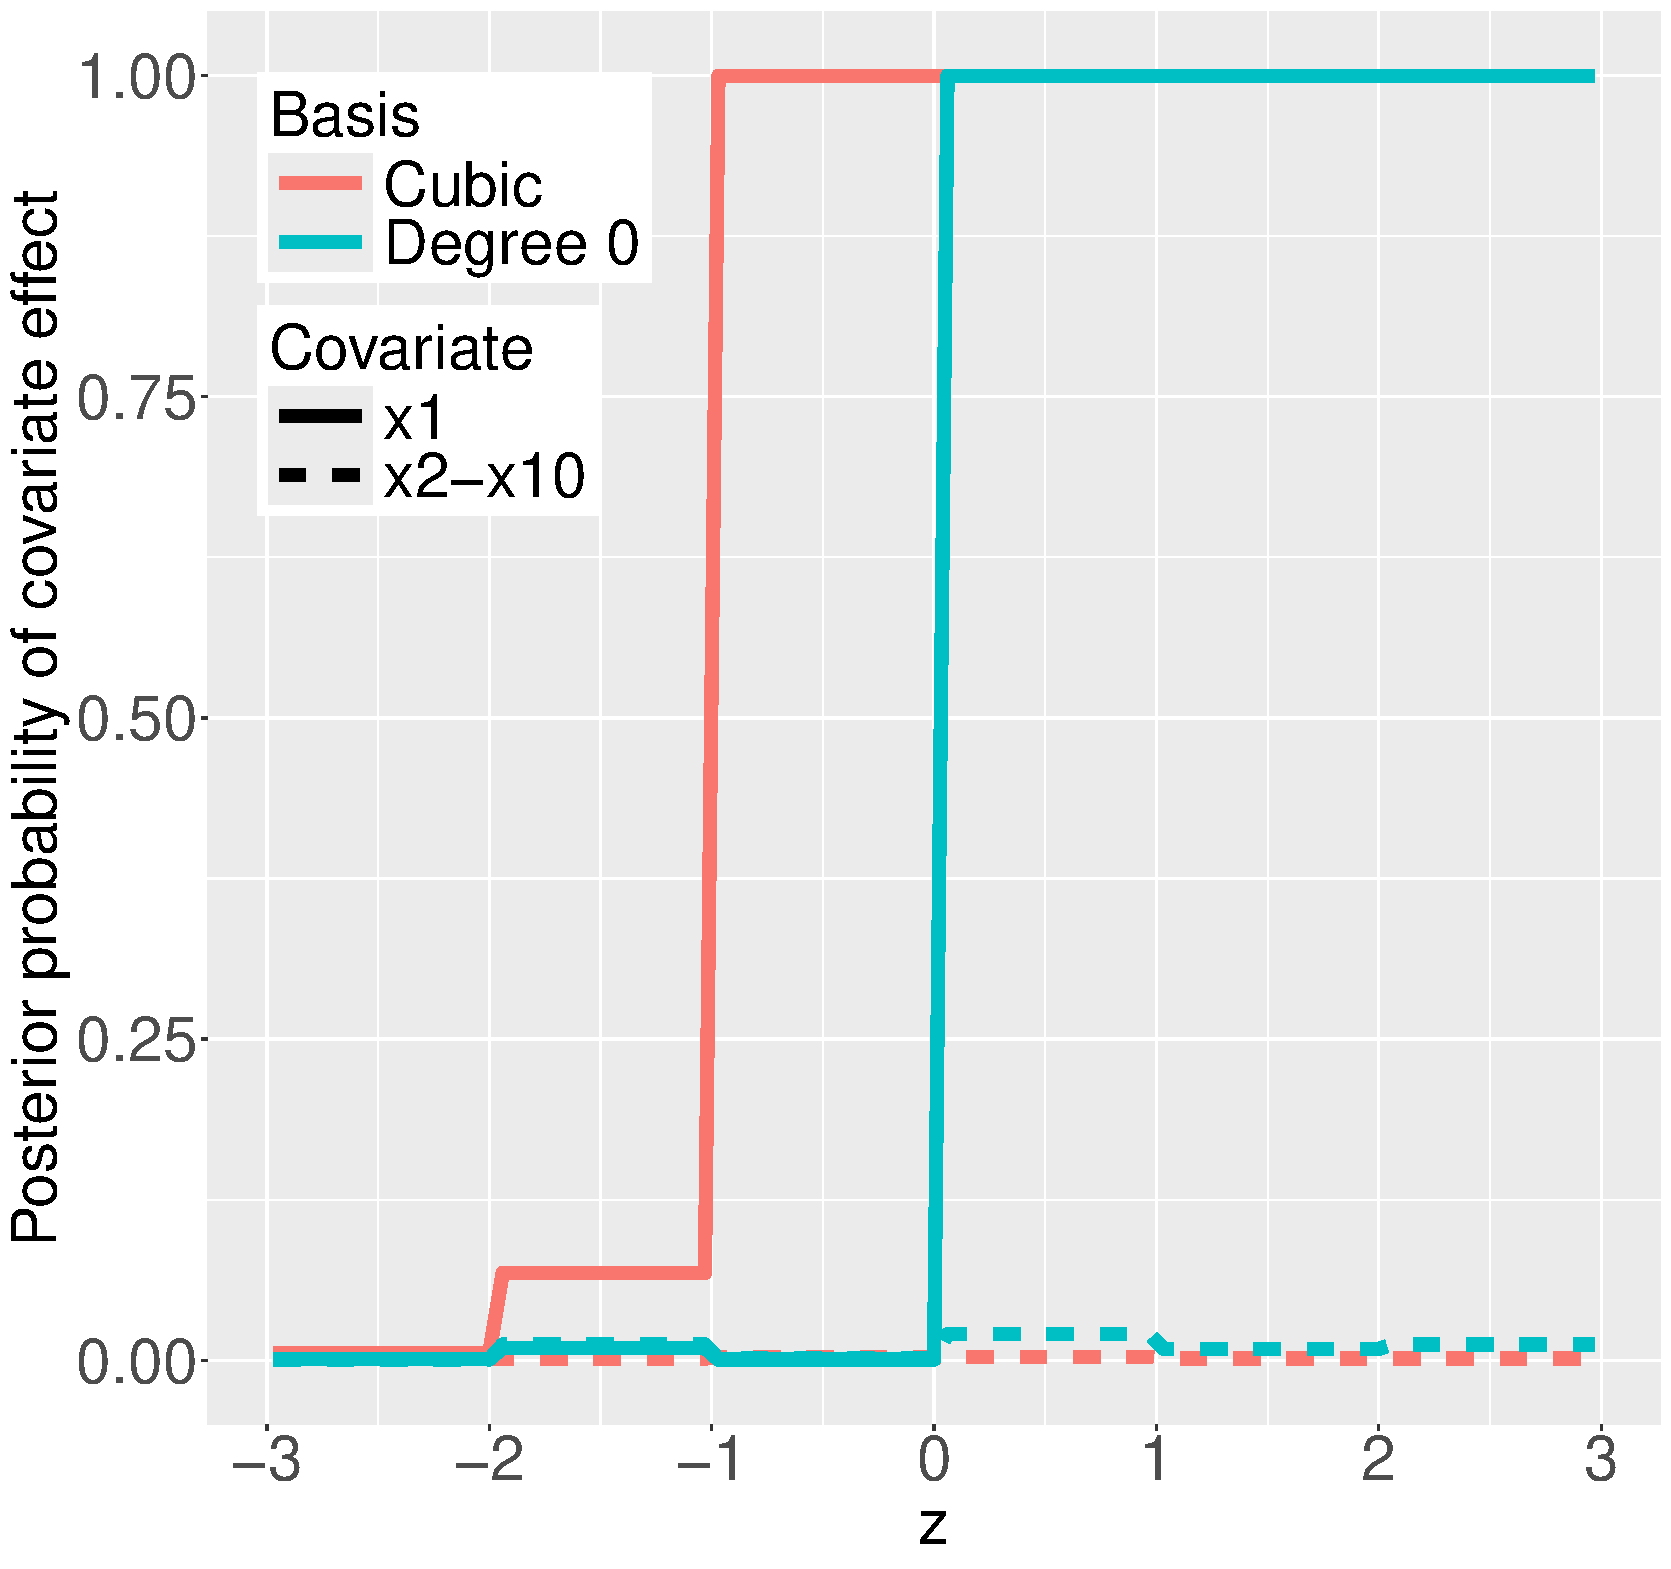
\includegraphics[width=0.5\textwidth,height=0.4\textwidth]{figs/simiid_unaligned_pp_n1000.pdf} \\
\end{tabular}
\end{center}
\caption{ Independent errors simulation with unaligned knots. 
Data-generating truth (top), and average
posterior probability for a local effect for $n=100$ (middle) and $n=1,000$ (bottom) }
\label{fig:simiid_unaligned}
\end{figure}




\subsection{Simulation with independent errors, non equi-spaced knots}
\label{ssec:simulation_iid_nonequispaced}


We illustrate our methodology in a setting where some of the resolutions place non equi-spaced knots for $\beta_1(z)$, the effect of a binary covariate.
The data-generating truth and the knots for the four considered resolution levels are depicted in Figure \ref{fig:simiid_nonequispaced}, top left panel.
The simulation settings are as in Section \ref{ssec:simulation_iid_misalign}, except that here we consider a single covariate for simplicity, and an increased range of sample sizes $n = \{100,1000,5000\}$.
In particular, note that the knots are misaligned with the true change point at $z=0.15$.
Resolutions 1 and 3 are equi-spaced and set a total of 7 and 11 knots, respectively.
Resolutions 2 and 4 place the same knots as resolution 1 and 3 (respectively) for $z<0$, and twice as many knots for $z>0$.

The right panel in Figure \ref{fig:simiid_nonequispaced} shows the average posterior probability for a local covariate effect for each sample size.
The results are analogous to those in Figure \ref{fig:simiid_unaligned} where only equi-spaced knots were considered.

The bottom panel in Figure \ref{fig:simiid_nonequispaced} show the average posterior probability assigned to the 4 resolutions.
As expected, for the smaller sample size $n=100$ the more parsimonious resolution 1 is favored. For $n=1000$, resolutions 2 and 3 receive more posterior probability. Intuitively, this occurs because the larger numbers of knots in these resolutions allow approximating $\beta_1(z)$ better, and the sample size is large enough to estimate the corresponding parameters accurately enough.
Similarly, for $n=5000$ it is resolutions 2 and 4 which receive the most posterior probability. This is appealing, since these resolutions place more knots at $z>0$ where the data-generating $\beta_1(z)$ varies, and less knots for $z<0$ where $\beta_1(z)=0$ is constant.


\begin{figure}
\begin{center}
\begin{tabular}{cccc}
\multicolumn{2}{c}{Data-generating truth}      & \multicolumn{2}{c}{$P(\beta_1(z) \neq 0 \mid y)$} \\
\multicolumn{2}{c}{and knots for 4 resolutions}& \multicolumn{2}{c}{}\\
\multicolumn{2}{c}{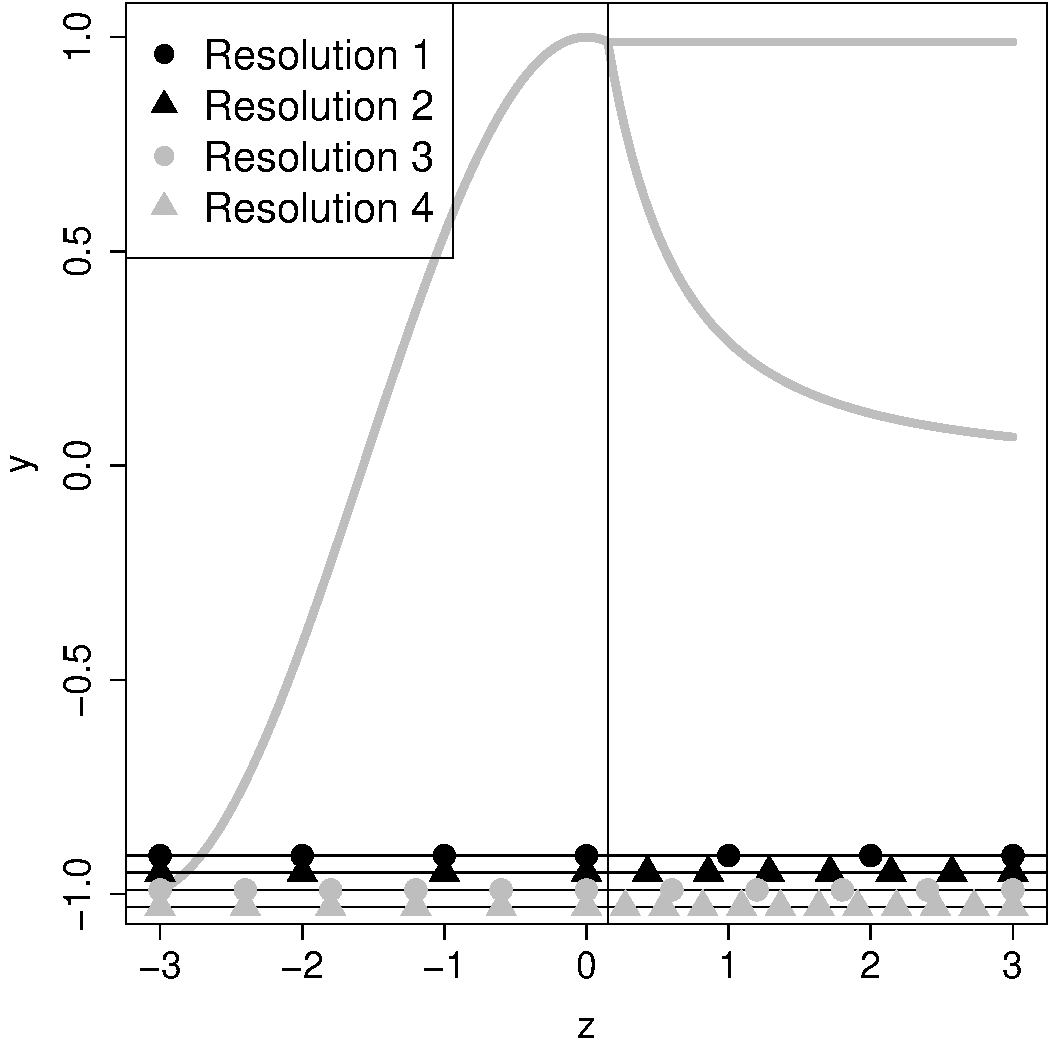
\includegraphics[width=0.5\textwidth]{figs/simiid_unaligned_nonequispaced.pdf}} &
\multicolumn{2}{c}{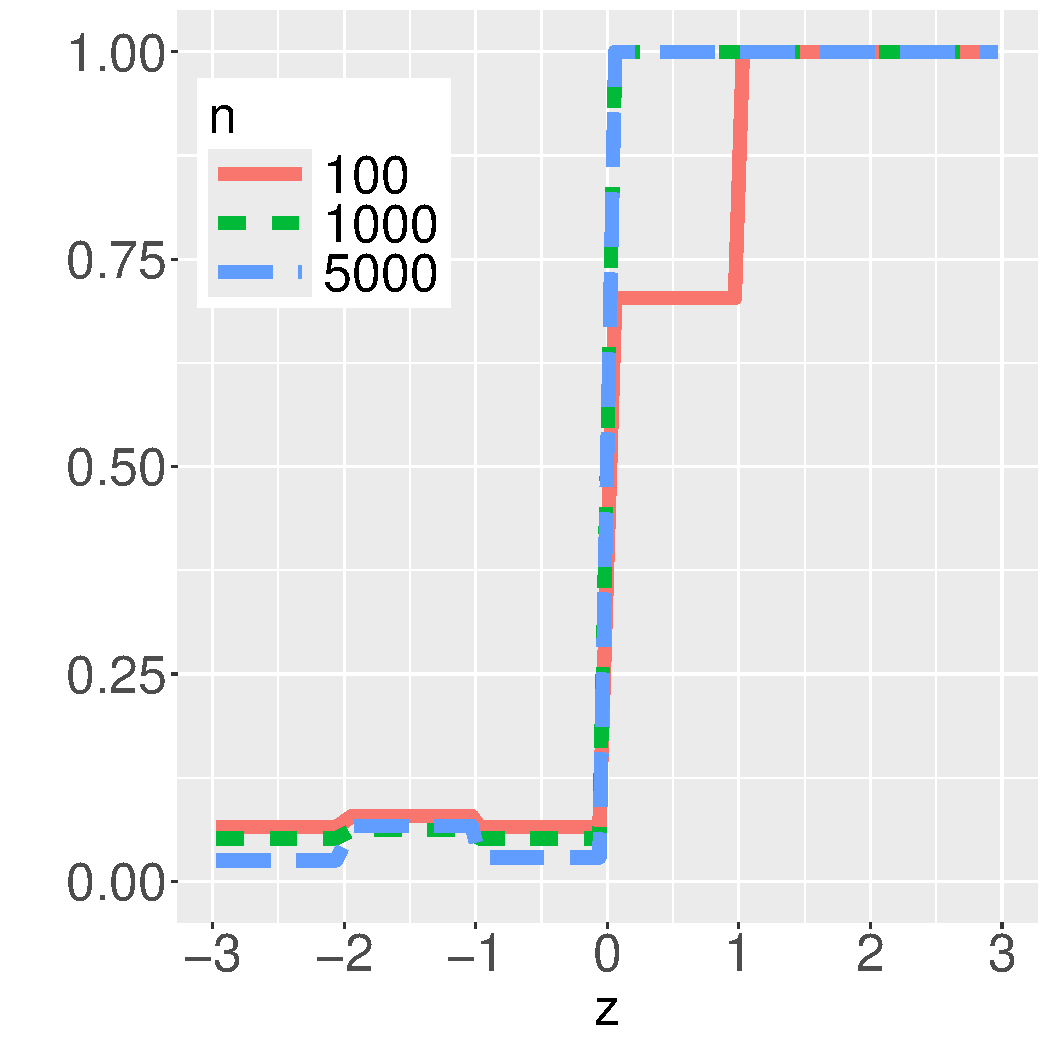
\includegraphics[width=0.5\textwidth]{figs/simiid_unaligned_nonequispaced_pp.pdf}} \\
& & & \\ %\hline
                             &  $n=100$ &  $n=1000$ &  $n=5000$ \\ %\hline
   Resolution 1  &  0.86    &  0.21     &  0.00     \\ 
   Resolution 2  &  0.01    &  0.30     &  0.55     \\ 
   Resolution 3  &  0.13    &  0.49     &  0.03     \\ 
   Resolution 4  &  0.00    &  0.00     &  0.42     \\  %\hline
\end{tabular}
\end{center}
\caption{ Independent errors simulation with non-equispaced knots.
Top left: data-generating truth and four resolutions. Resolutions 1 and 3 have the same number of knots for $z<0$ and $z>0$.
Resolutions 2 and 4 have twice as many knots for $z>0$.
Top right: average $P(\beta_1(z) \neq 0 \mid y)$ for $n=100$, $n=1,000$ and $n=5,000$.
Bottom: average posterior probability assigned to each resolution
 }
\label{fig:simiid_nonequispaced}
\end{figure}


%\begin{figure}
%\begin{center}
%\begin{tabular}{cc}
%Data-generating truth &  $P(\beta_1(z) \neq 0 \mid y)$ \\
%and knots for 4 resolutions & \\
%
\includegraphics[width=0.5\textwidth]{../../figs/simiid_unaligned_nonequispaced.pdf} &
%
\includegraphics[width=0.5\textwidth]{../../figs/simiid_unaligned_nonequispaced_pp.pdf} \\
%\end{tabular}
%\end{center}
%\caption{ Independent errors simulation with non-equispaced knots.
%Left: data-generating truth and four resolutions. Resolutions 1 and 3 have the same number of knots for $z<0$ and $z>0$.
%Resolutions 2 and 4 have twice as many knots for $z>0$.
%Right: average $P(\beta_1(z) \neq 0 \mid y)$ for $n=100$, $n=1,000$ and $n=5,000$ }
%\label{fig:simiid_nonequispaced}
%\end{figure}


%\begin{table}
%\begin{center}
%\begin{tabular}{lccc} %\hline
%                                              & n=100 & n=1000 & n=5000 \\ %\hline
%   7 knots, equi-spaced                       & 0.86 & 0.21 & 0.00 \\ 
%  11 knots (3 regions for z$<$0, 7 for z$>$0) & 0.01 & 0.30 & 0.55 \\ 
%  11 knots, equi-spaced                       & 0.13 & 0.49 & 0.03 \\ 
%  17 knots (5 regions for z$<$0, 11 for z$>$0) & 0.00 & 0.00 & 0.42 \\ 
%   %\hline
%\end{tabular}
%\end{center}
%\caption{Average posterior probability assigned to the 4 resolutions in Figure \ref{fig:simiid_nonequispaced}.}
%\label{tab:pp_localknots}
%\end{table}




\subsection{Simulation with independent errors, bivariate $z$}
\label{ssec:simulation_iid_bivar}


\begin{figure}
\begin{center}
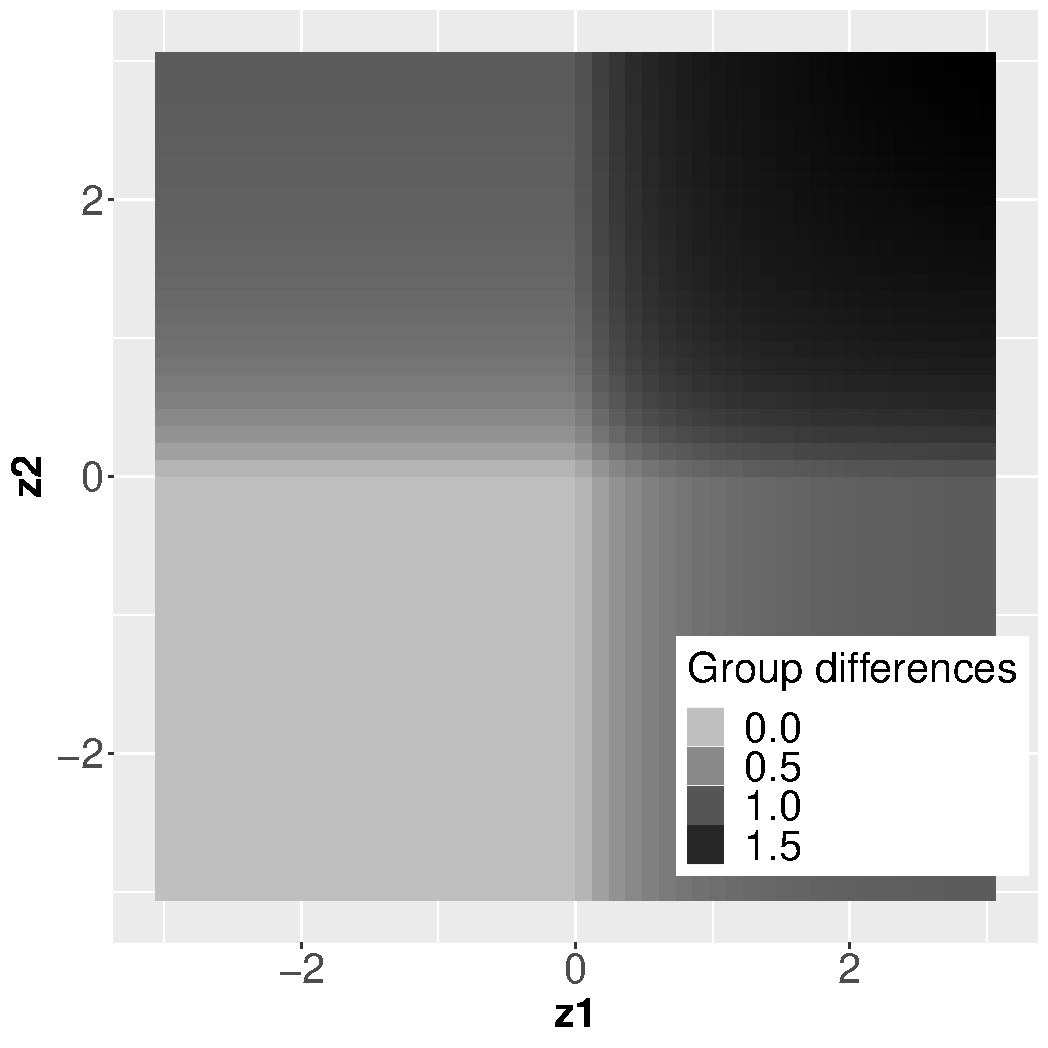
\includegraphics[width=0.6\textwidth]{figs/bspline_fit_cubic_bivar.pdf}
\end{center}
\caption{True group mean differences $E_F(y_i \mid x_{i1}=1, z_i) - E_F(y_i \mid x_{i1}=0, z_i)$ in bivariate $z$ simulation}
\label{fig:bspline_fit_cubic_bivar}
\end{figure}

\begin{figure}
\begin{center}
Covariate 1 \\
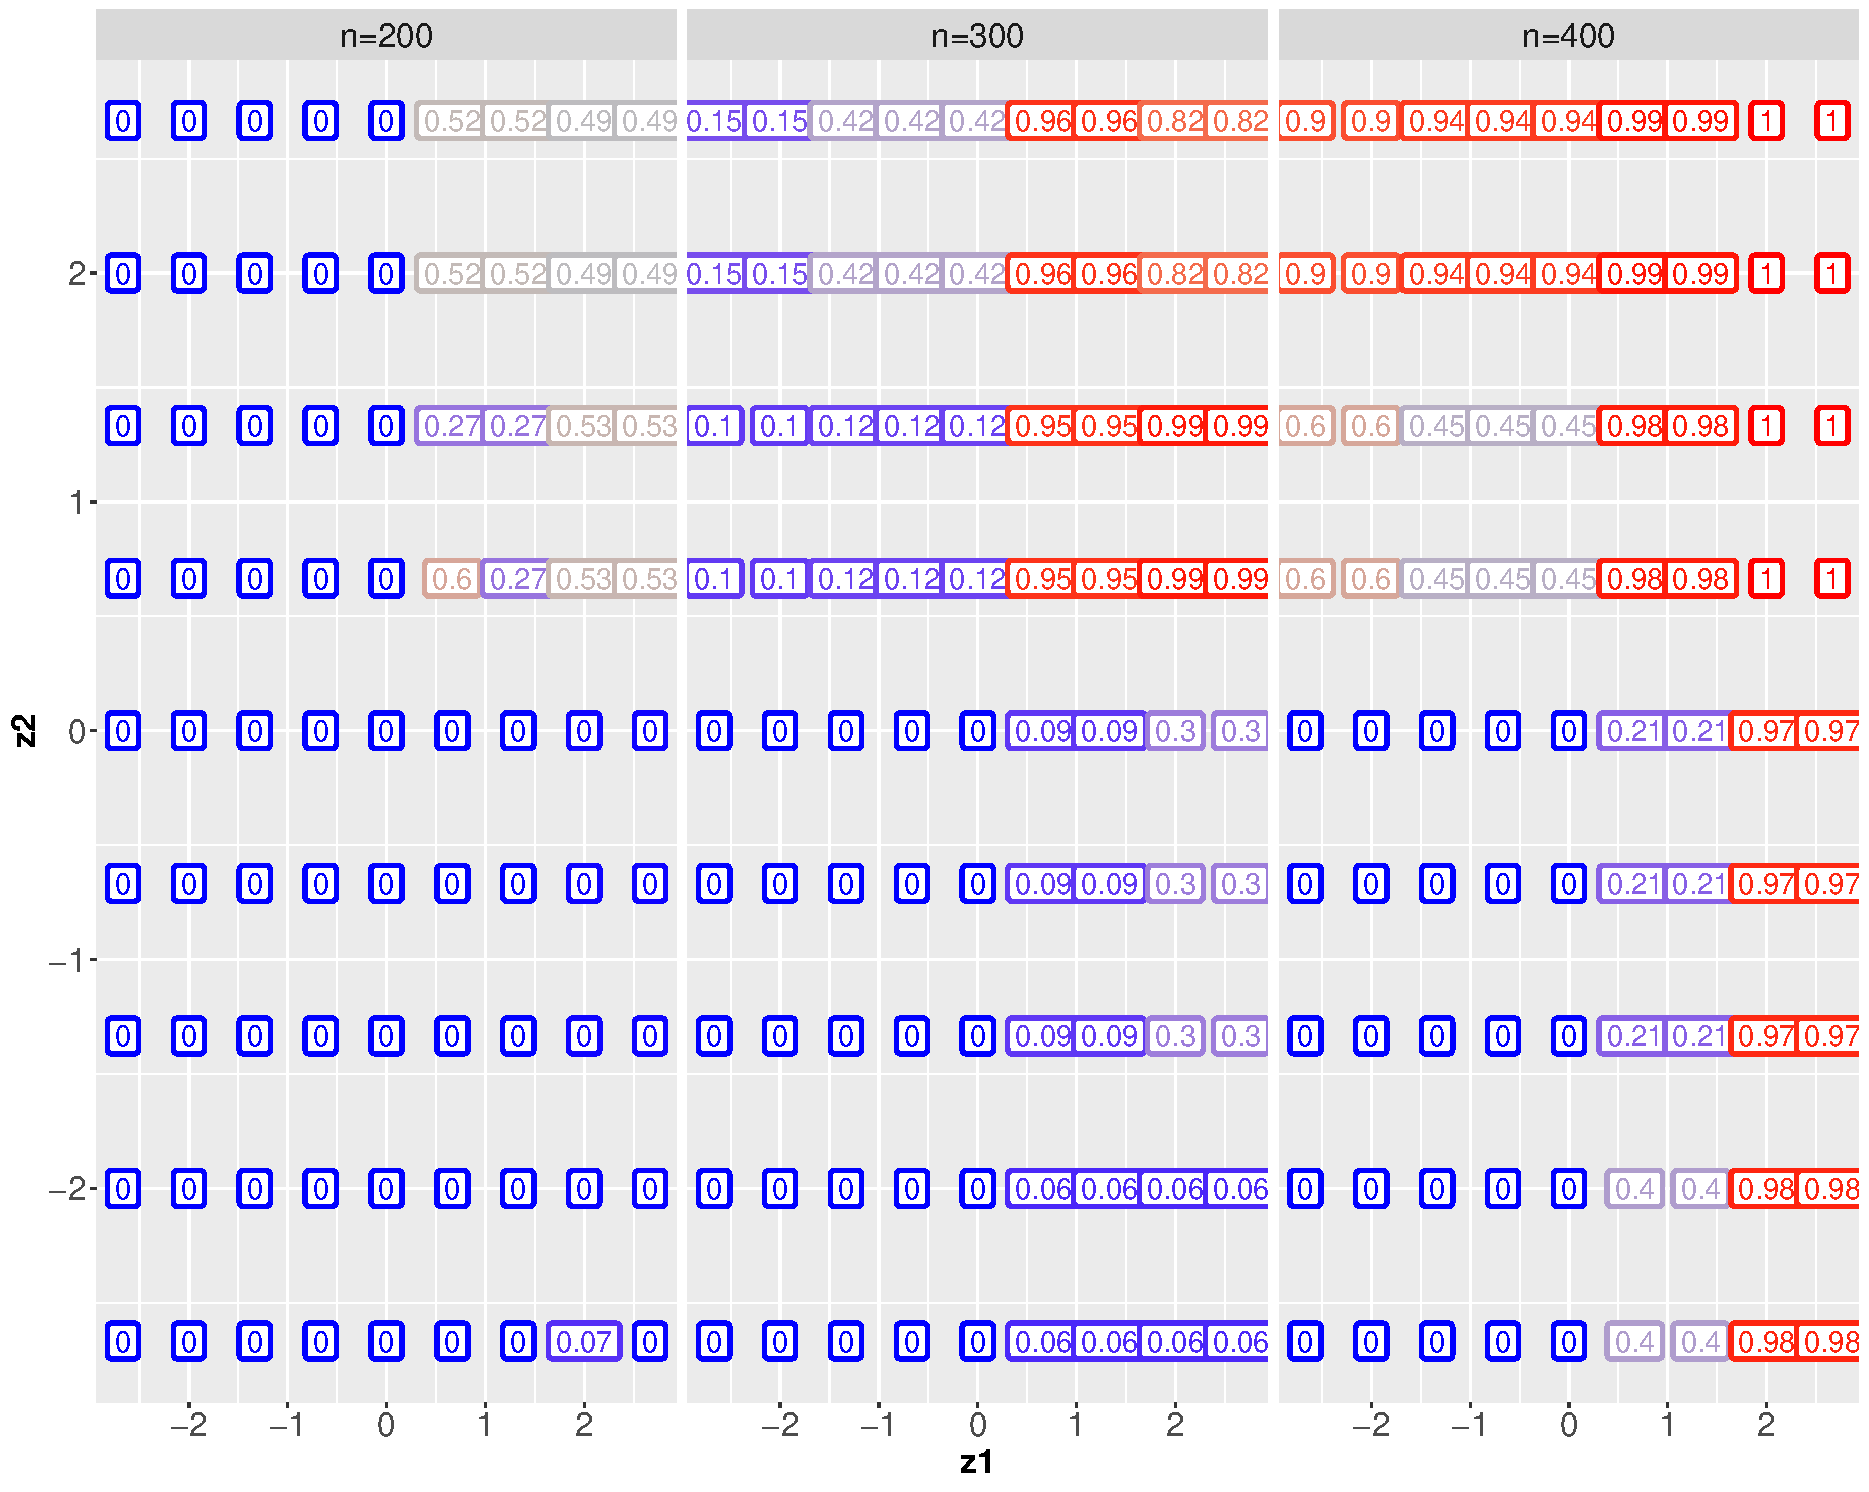
\includegraphics[width=1\textwidth, height=0.65\textwidth]{figs/simiid_pp_bivar_x1.pdf} \\
Covariates 2-10 \\
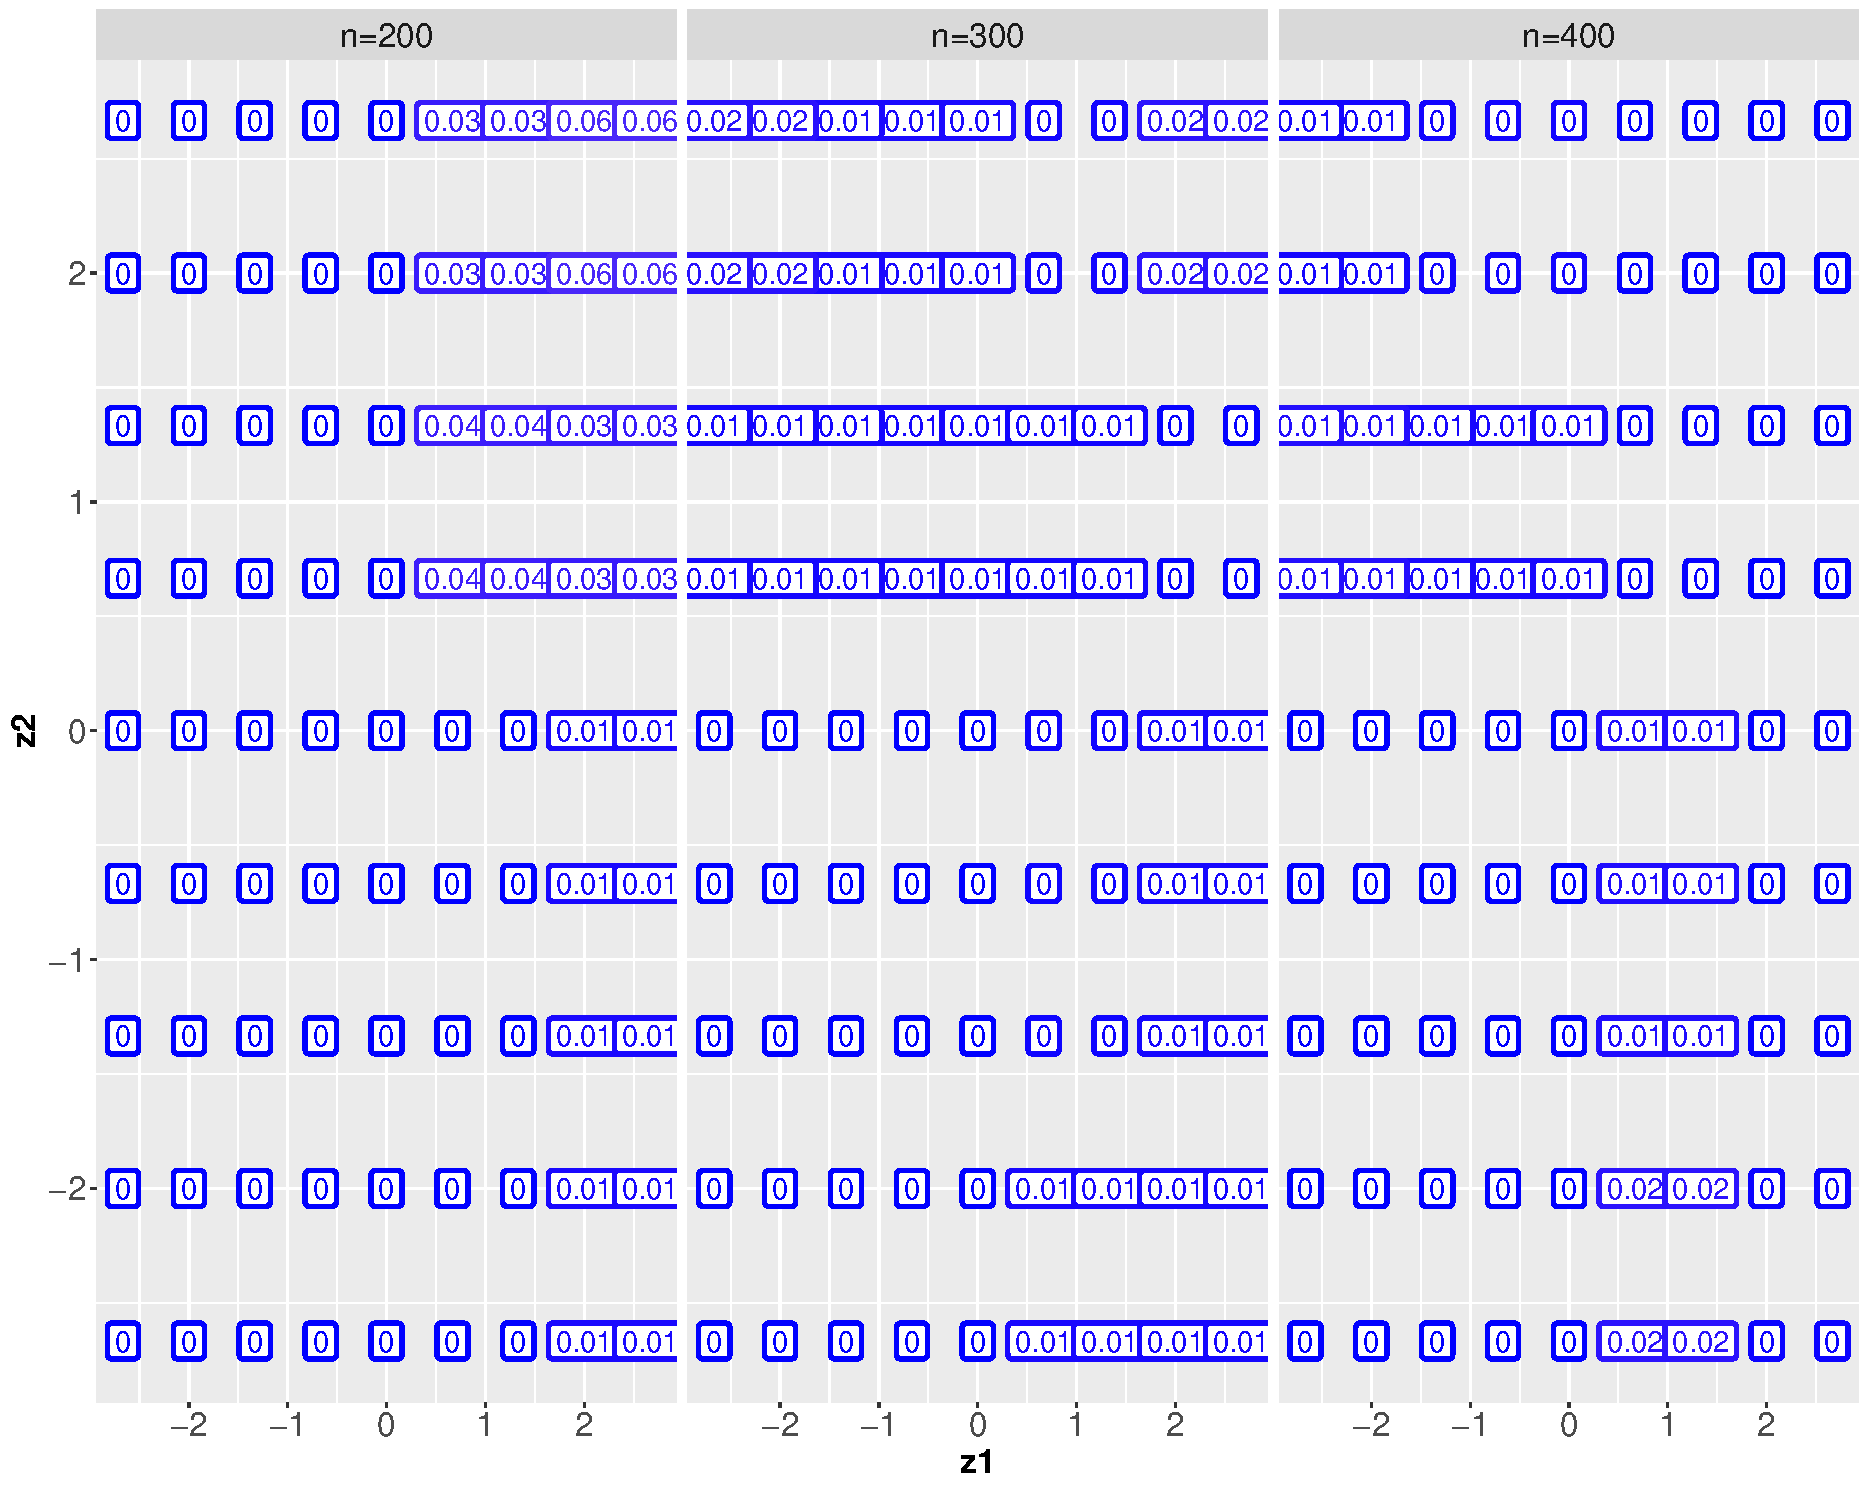
\includegraphics[width=1\textwidth, height=0.65\textwidth]{figs/simiid_pp_bivar_xother.pdf}
\end{center}
\caption{Simulation example with bivariate $z$ for $p=10$, $n=200, 300, 400$.
Posterior probabilities for a local effect of covariate 1 (truly active if $z_1>0$ or $z_2>0$) and inactive covariates 2-10}
\label{fig:simiid_bivar}
\end{figure}


Figure \ref{fig:simiid_bivar} shows a simulation study with bivariate $z$ that extends that presented in Section \ref{sec:simulation_iid}. The results are averaged across 50 independent simulations.
 We used a multi-resolution analysis that placed 5, 10 and 15 knots in each of the two dimensions. The average run time was 20 seconds using 1 core and 10 seconds using 3 cores on an Ubuntu Linux desktop, 13th Gen Intel core i7 processor, with 32Gb RAM. 
As in Section \ref{sec:simulation_iid} we consider $p=10$ covariates where $x_{i1}$ is binary and the remaining covariates $x_{i2},\ldots,x_{ip}$ are Gaussian, correlated with $x_{i1}$, and truly have no effect on the outcome. 
The true mean is set such that covariate $x_{i1}$ has an effect whenever $z_{i1}>0$ or $z_{i2}>0$.
Specifically, the true mean for group $x_{i1}=1$ is
\begin{align}
E_F(y_i \mid x_{i1}=0, z_i)= 
\sum_{j=1}^2 \mbox{I}(z_{ij} \leq 0) \cos(z_{ij}) + \mbox{I}(z_{ij} \leq 0)
\nonumber
\end{align}
In contrast, for group $x_{i1}=0$ it is
\begin{align}
E_F(y_i \mid x_{i1}=0, z_i)= 
\sum_{j=1}^2 \mbox{I}(z_{ij} \leq 0) \cos(z_{ij}) + \mbox{I}(z_{ij} \leq 0) \frac{1}{(z_{ij}^2+1)^2}.
\nonumber
\end{align}
That is, the setting is akin to that in the top panels of Figure \ref{fig:splinefit}, with bivariate $z$. 
Figure \ref{fig:bspline_fit_cubic_bivar} shows the group differences $E_F(y_i \mid x_{i1}=1, z_i) - E_F(y_i \mid x_{i1}=0, z_i)$.
We consider sample sizes $n \in \{200, 300, 400\}$, which suffice to illustrate the transition from a low- to a high-power setting.

The top panel in Figure \ref{fig:simiid_bivar} show that for $n=200$ the average marginal posterior probabilities for $x_{i1}$ are nearly zero, except for the region $(z_{i1}>0, z_{i2}>0)$, where the group differences are larger.
For $n=300$ and $n=400$ said posterior probabilities grow closer to 1 whenever there are truly group differences, but remain close to 0 for $(z_{i1}<0, z_{i2}<0)$ where there are no group differences.
The bottom panel shows how for covariates 2-10 the marginal probabilities remain close to zero for all $(z_{i1},z_{i2})$, indicating that the type I error probability is satisfactorily controlled.



\subsection{Functional data simulation}
\label{ssec:simulation_fda}

\begin{table}
\begin{center}
\begin{tabular}{ccccc} %\hline
\multicolumn{5}{c}{$M=50$ individuals}        \\ %\hline
& \multicolumn{2}{c}{Cut degree 0} & \multicolumn{2}{c}{VC-BART} \\
 Region         & Covariate 1 & Covariates 2-10 &  Covariate 1  &  Covariates 2-10  \\
$z \in $(-3,-2] & 0.06         & 0.080          &  0.60         &  0.58 \\ 
$z \in $(-2,-1] & 0.06         & 0.078          &  0.61         &  0.57 \\ 
$z \in $(-1,0]  & 0.056        & 0.072          &  0.61         &  0.58 \\ 
$z \in $(0,1]   & 0.73         & 0.084          &  0.82         &  0.56 \\ 
$z \in $(1,2]   & 0.873        & 0.070          &  0.97         &  0.56 \\ 
$z \in $(2,3]   & 1            & 0.057          &  0.98         &  0.54 \\ 
%\hline
\multicolumn{5}{c}{$M=100$ individuals} \\ %\hline
& \multicolumn{2}{c}{Cut degree 0} & \multicolumn{2}{c}{VC-BART} \\
 Region          & Covariate 1   & Covariates 2-10 &  Covariate 1 &  Covariates 2-10 \\
$z \in $ (-3,-2] & 0.05          & 0.036           &  0.64        &   0.58           \\
$z \in $ (-2,-1] & 0.045         & 0.038           &  0.72        &   0.52           \\ 
$z \in $ (-1,0]  & 0.0376        & 0.039           &  0.59        &   0.48           \\ 
$z \in $ (0,1]   & 0.99          & 0.036           &  0.89        &   0.52           \\ 
$z \in $ (1,2]   & 0.995         & 0.031           &  1           &   0.54           \\ 
$z \in $ (2,3]   & 1             & 0.027           &  1           &   0.51           \\ 
%\hline
\end{tabular}
\end{center}
\caption{Functional data simulation. Proportion of rejected null hypothesis for our 0-degree cut orthogonal basis,  and VC-BART.  For covariate 1 and $z>0$ this is the statistical power, otherwise it is the type I error}
\label{tab:simfda_10covar}
\end{table}


\begin{figure}
\begin{center}
\begin{tabular}{cc}
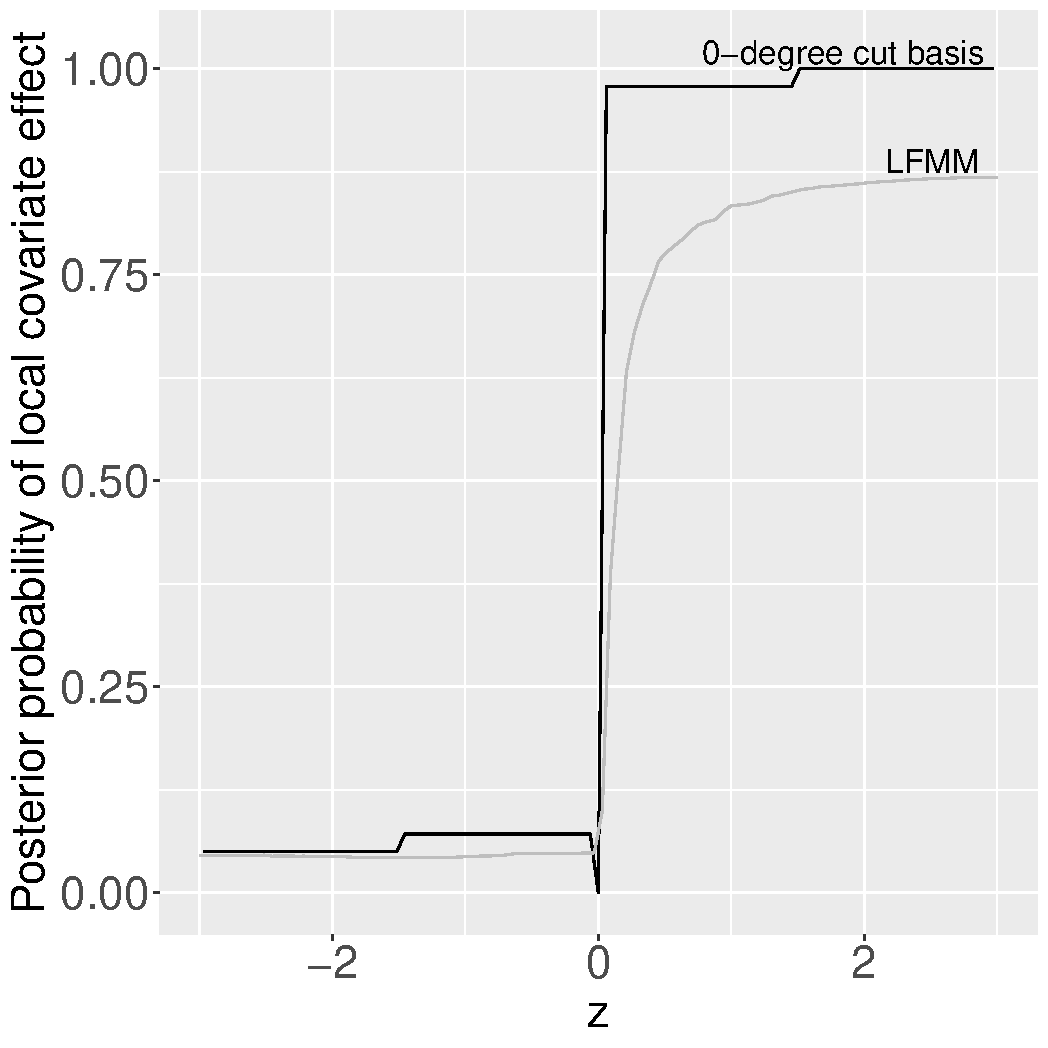
\includegraphics[width=0.48\textwidth]{figs/simfda_pp_single_nindiv50.pdf} &
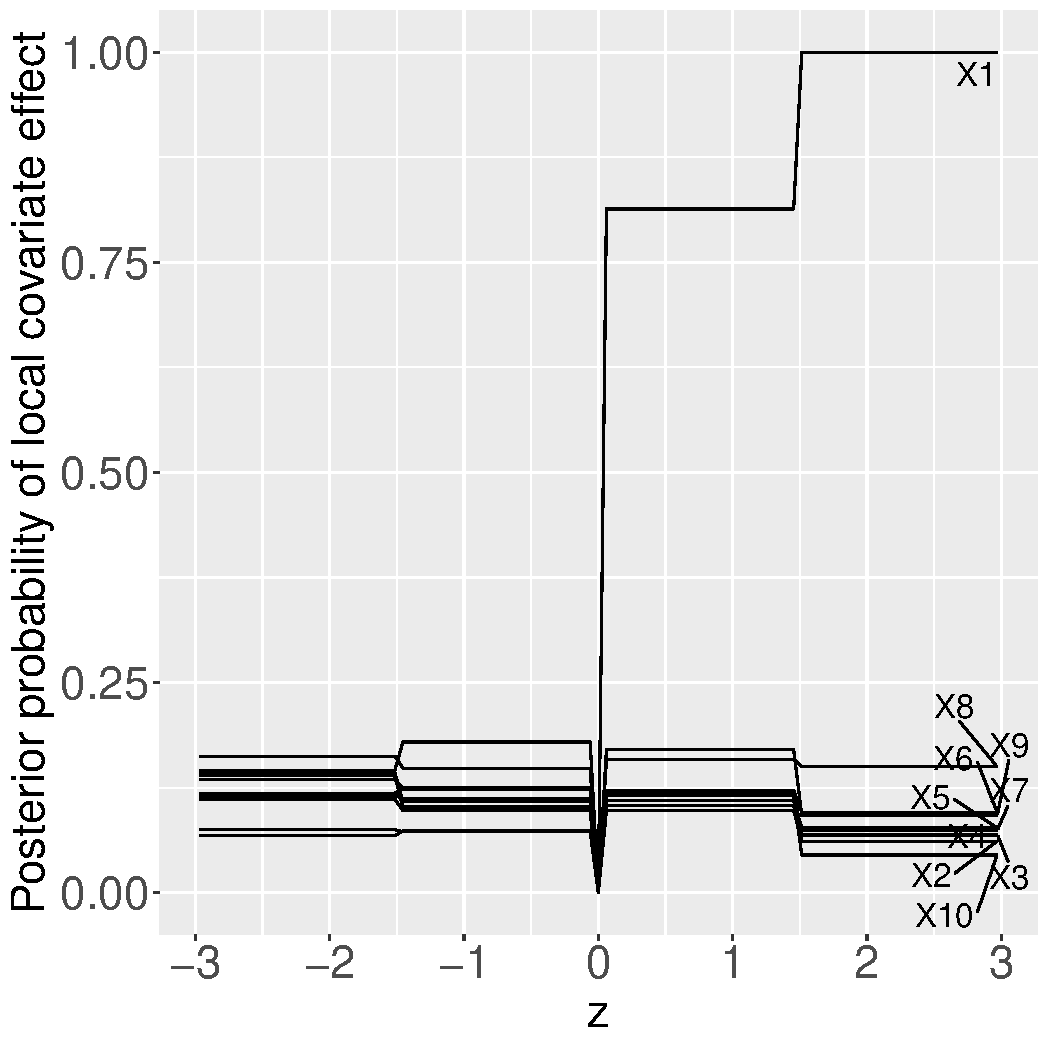
\includegraphics[width=0.48\textwidth]{figs/simfda_pp_nindiv50.pdf}
\end{tabular}
\end{center}
\caption{Functional data simulation. Posterior probability of a local covariate effect when using a single covariate (left) and 10 covariates (right)}
\label{fig:pp_simfda}
\end{figure}


Figure \ref{fig:pp_simfda} displays a comparison of the two Bayesian methods, our framework and tensor model (referred to by the acronym LFMM by its authors) proposed by \cite{paulon:2023}, in terms of the posterior probability assigned to the existence of a local covariate effect as a function of $z$ (averaged across 100 simulations).
The left panel is based on fitting the model where one only consider the truly active covariate 1, whereas the right panel also includes truly spurious covariates 2-10. Recall that covariate 1 truly has an effect only for $z>0$.


\subsection{Salary data}


\begin{figure}
\begin{center}
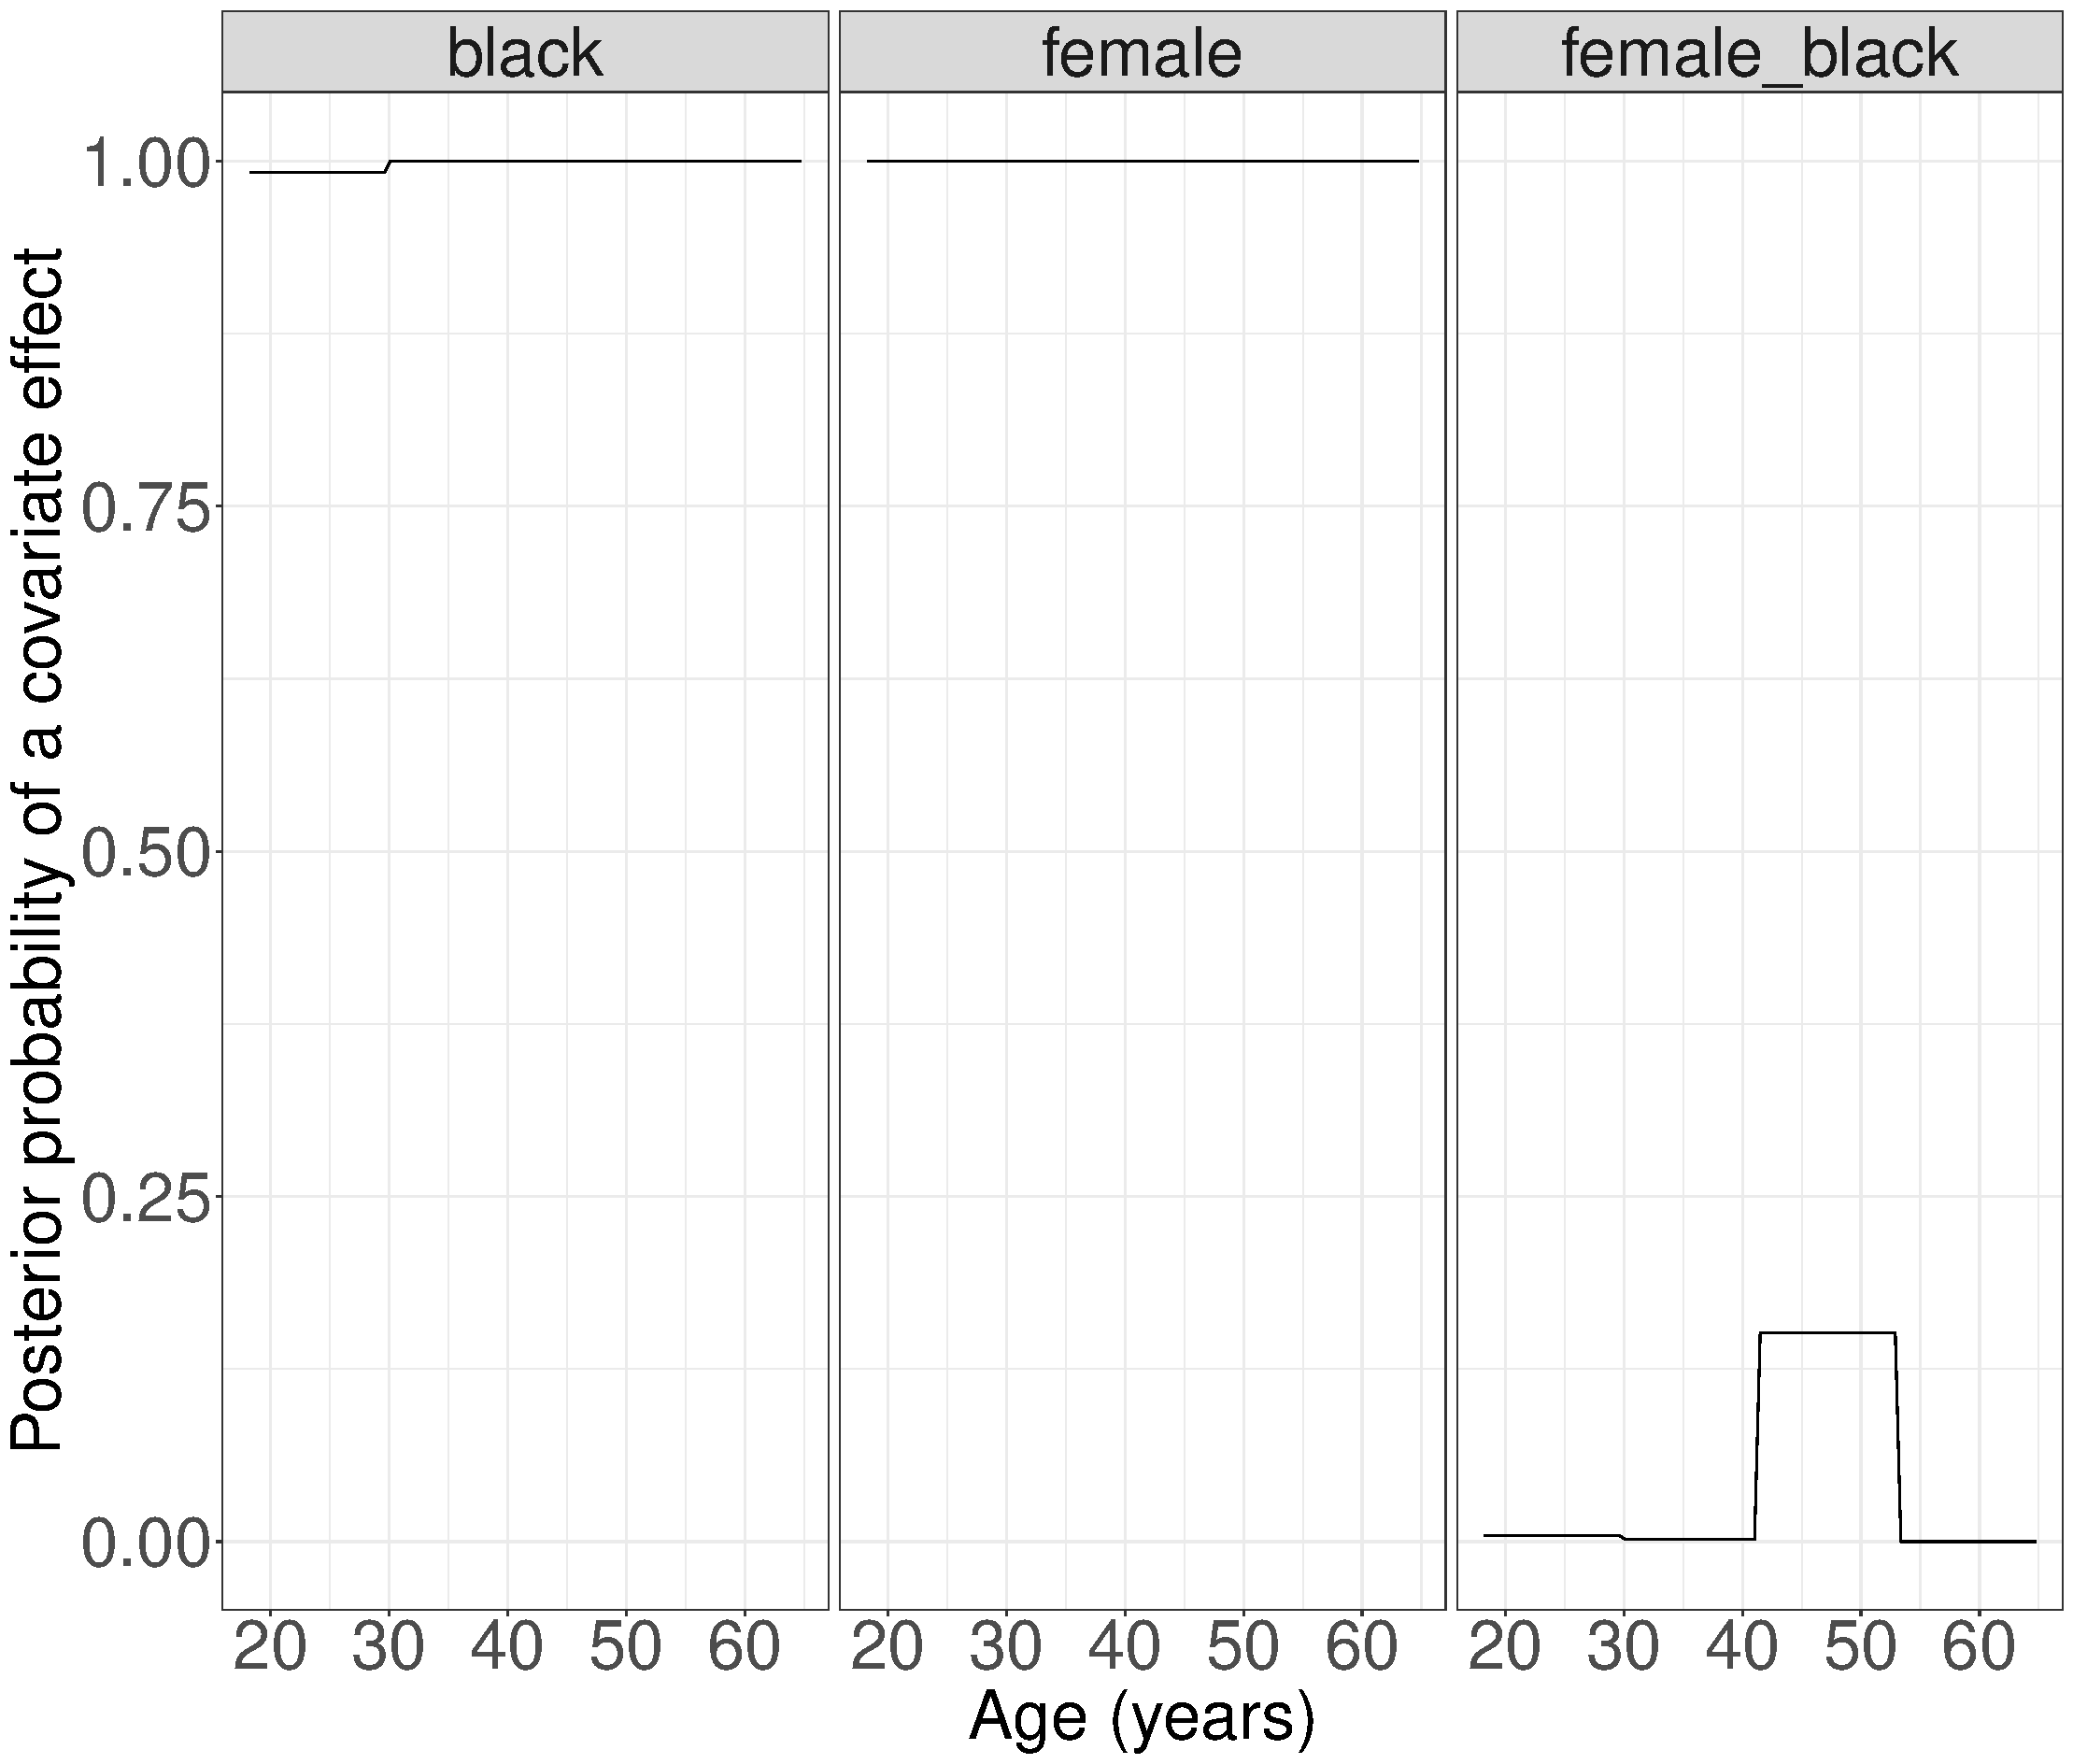
\includegraphics[width=0.7\textwidth]{figs/salary_pp_localtests_femaleblack.pdf}
\end{center}
\caption{Salary Data. Posterior probability of a salary gap associated with black race, sex and a black:sex interaction versus age, adjusted by occupation and worker class, and also including local effects for college, government, Hispanic race, and self-employment}
\label{fig:salary_female_race}
\end{figure}

\begin{figure}
\begin{center}
\begin{tabular}{cc}
\multicolumn{2}{c}{20 knots for baseline, 20 knots for local tests} \\
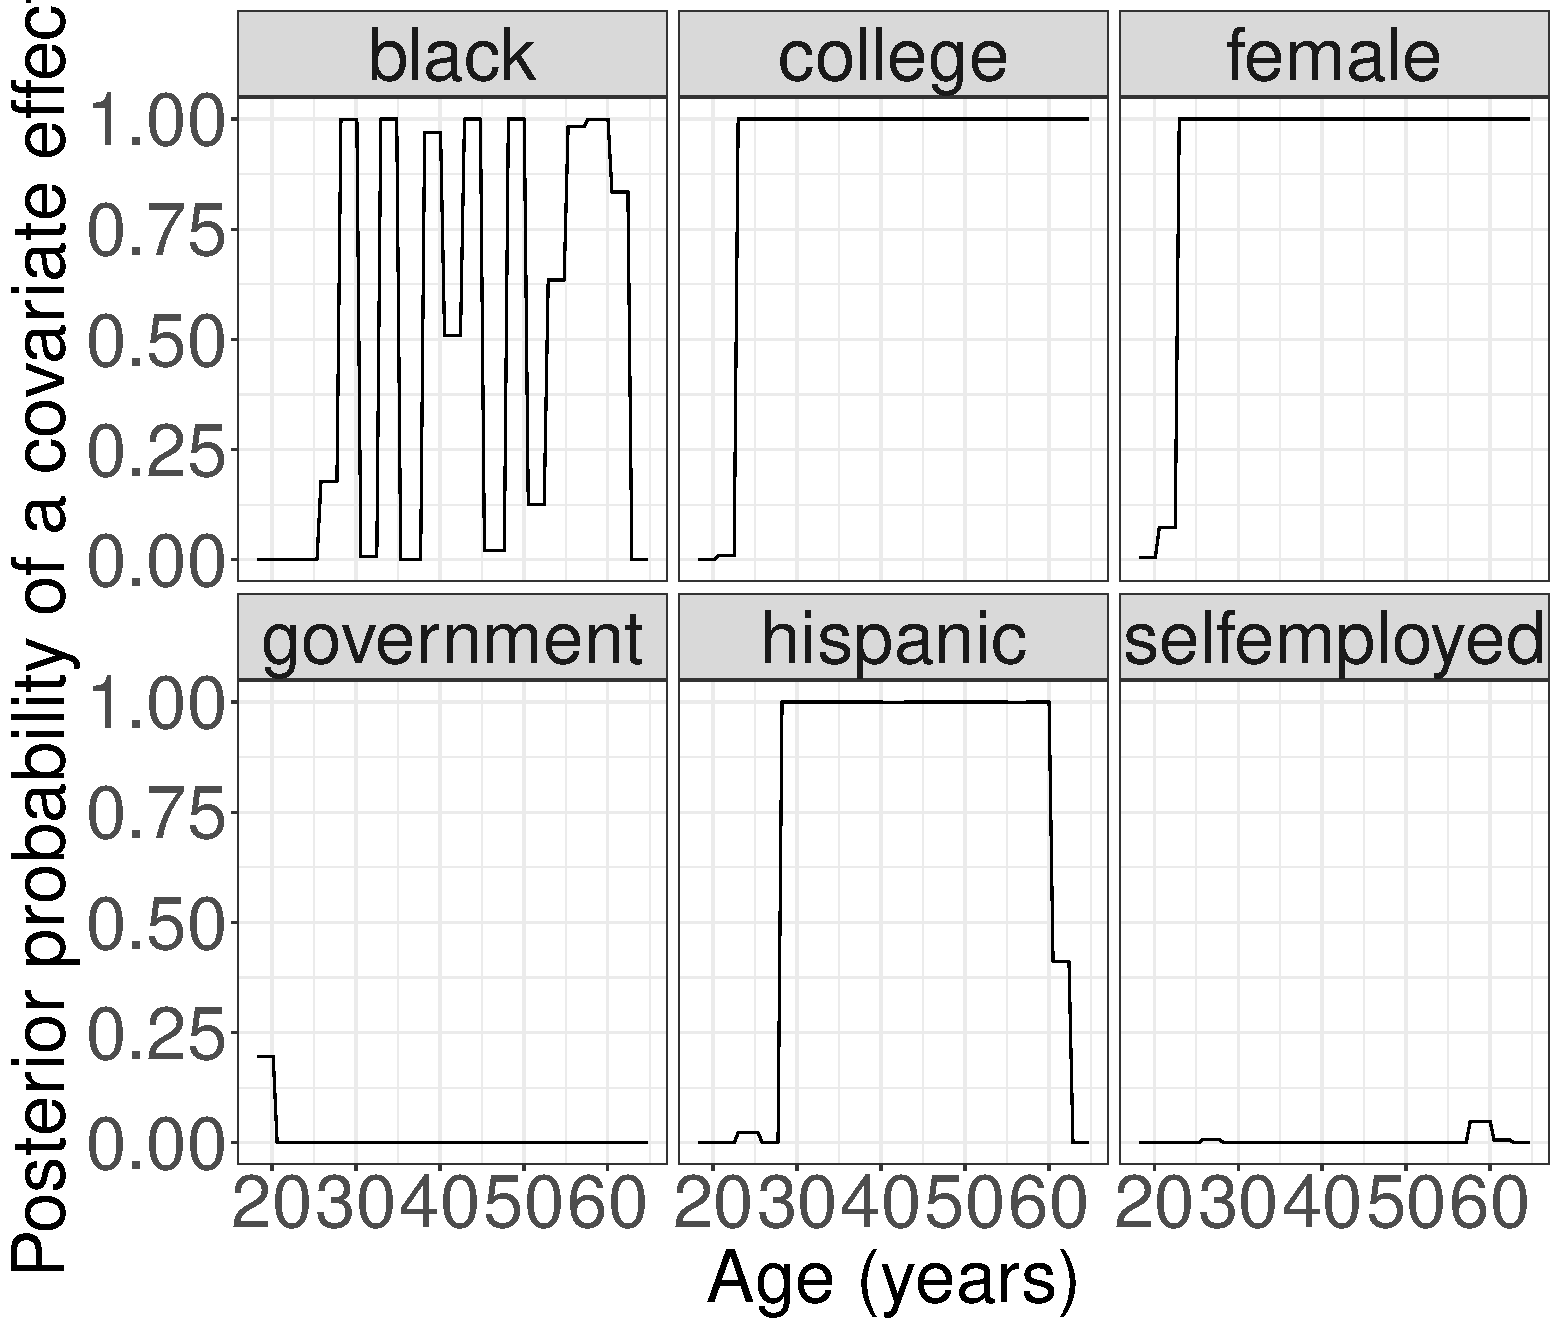
\includegraphics[width=0.5\textwidth]{figs/salary_pp_localtests_20knots.pdf} &
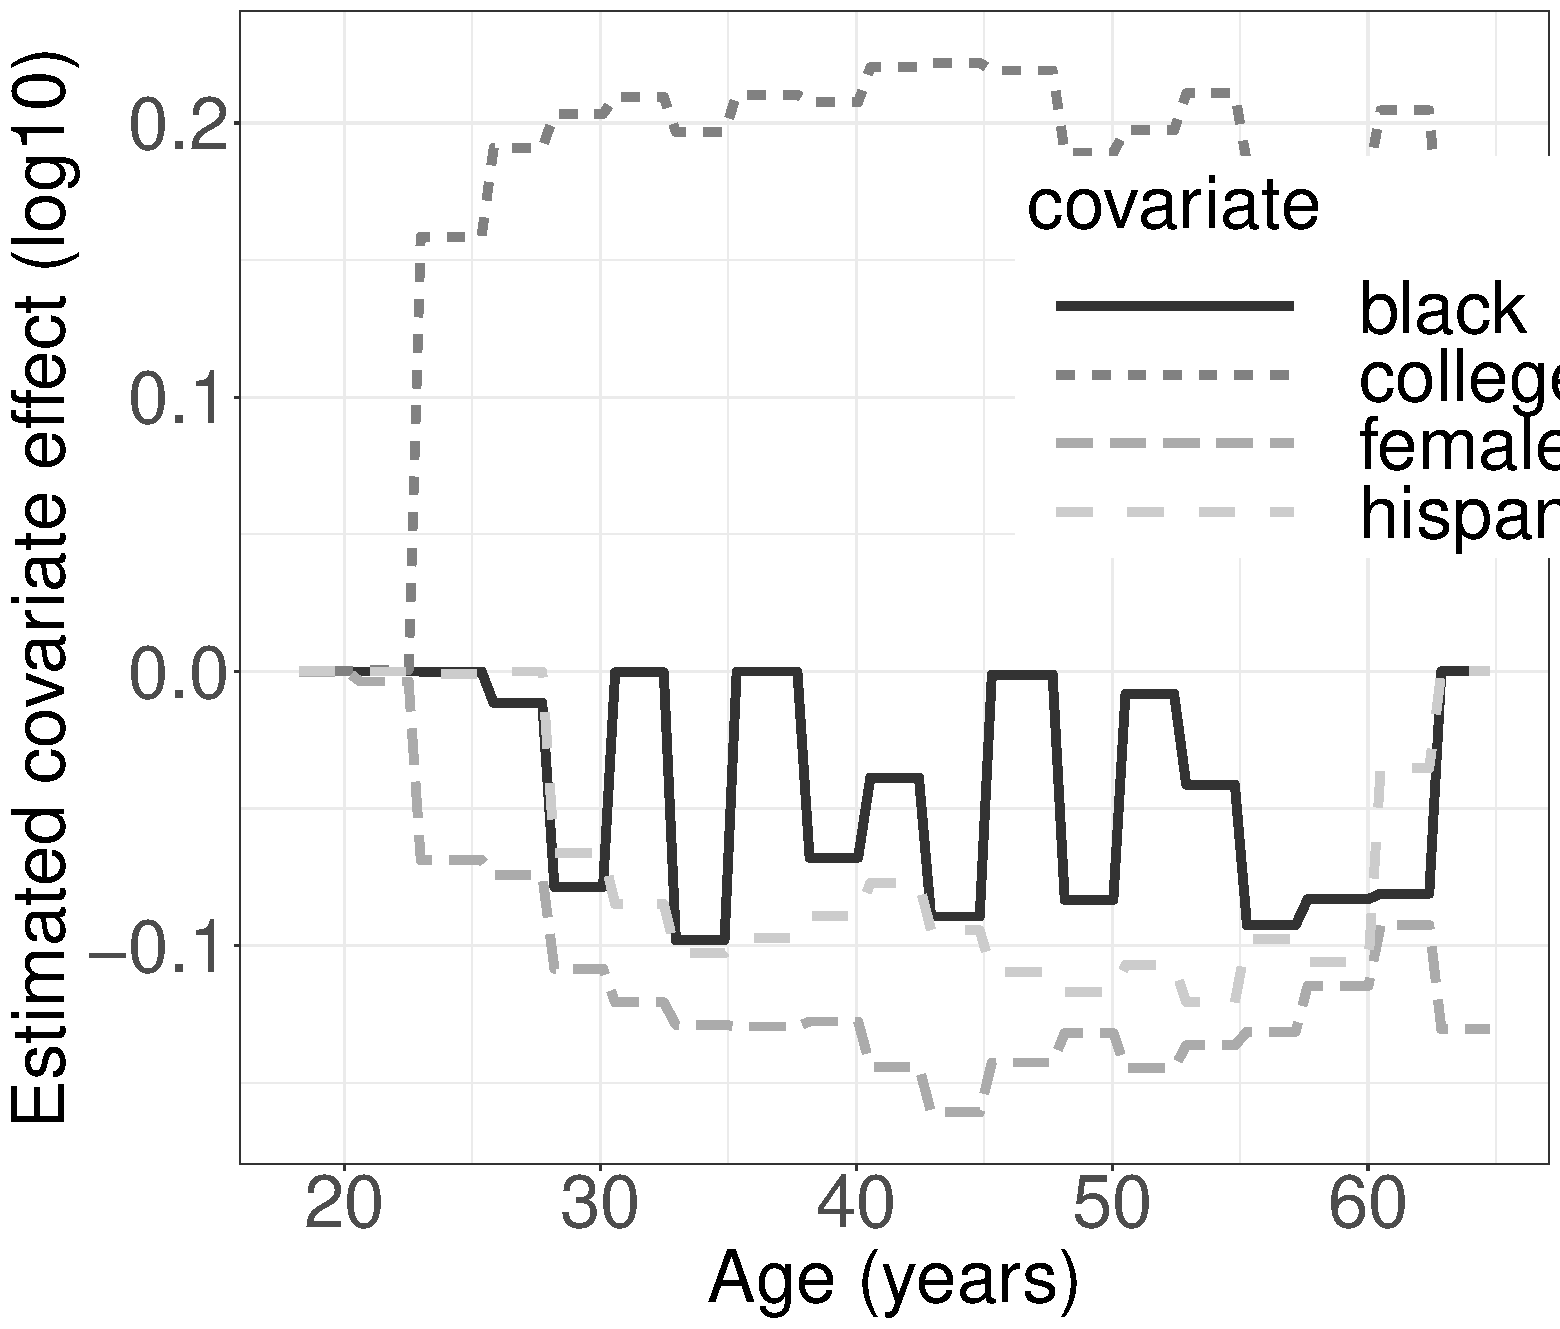
\includegraphics[width=0.5\textwidth]{figs/salary_estimated_effects_20knots.pdf} \\
%
\multicolumn{2}{c}{30 knots for baseline, 30 knots for local tests} \\
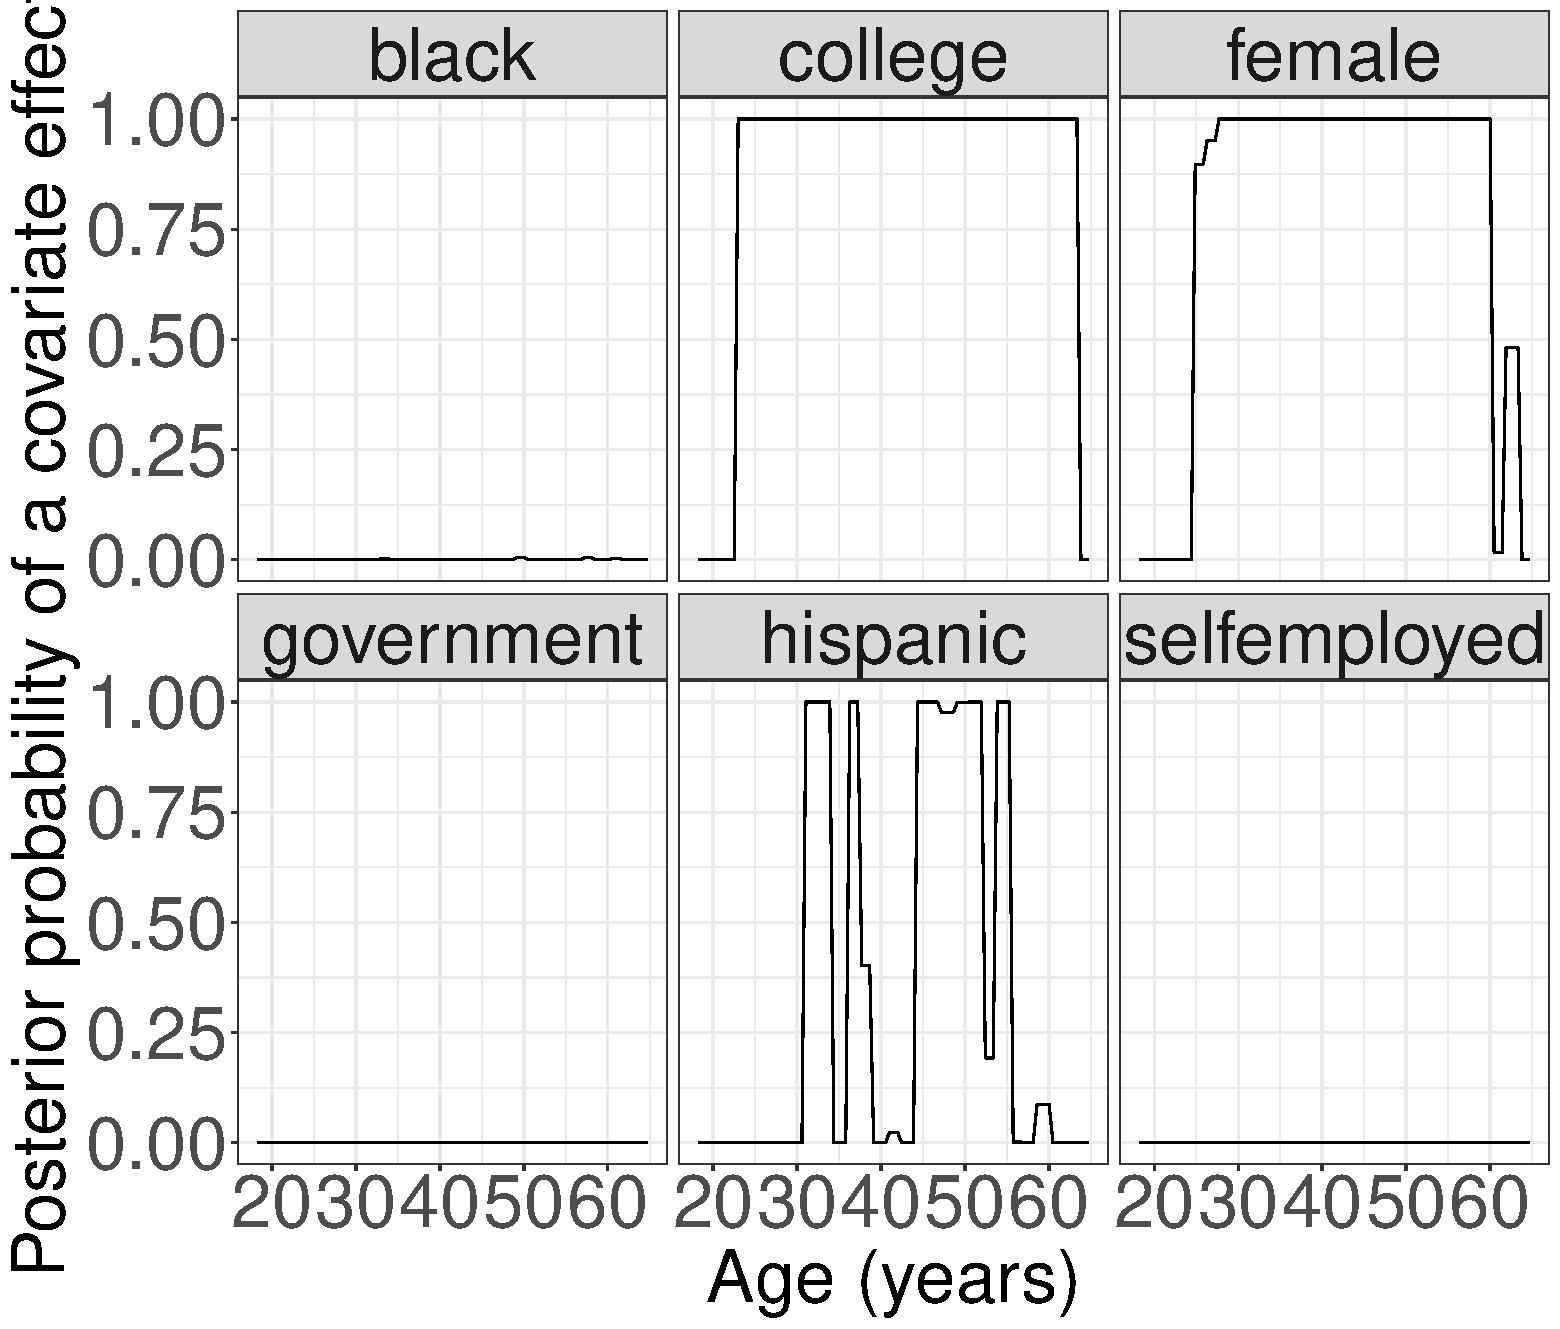
\includegraphics[width=0.5\textwidth]{figs/salary_pp_localtests_30knots.pdf} &
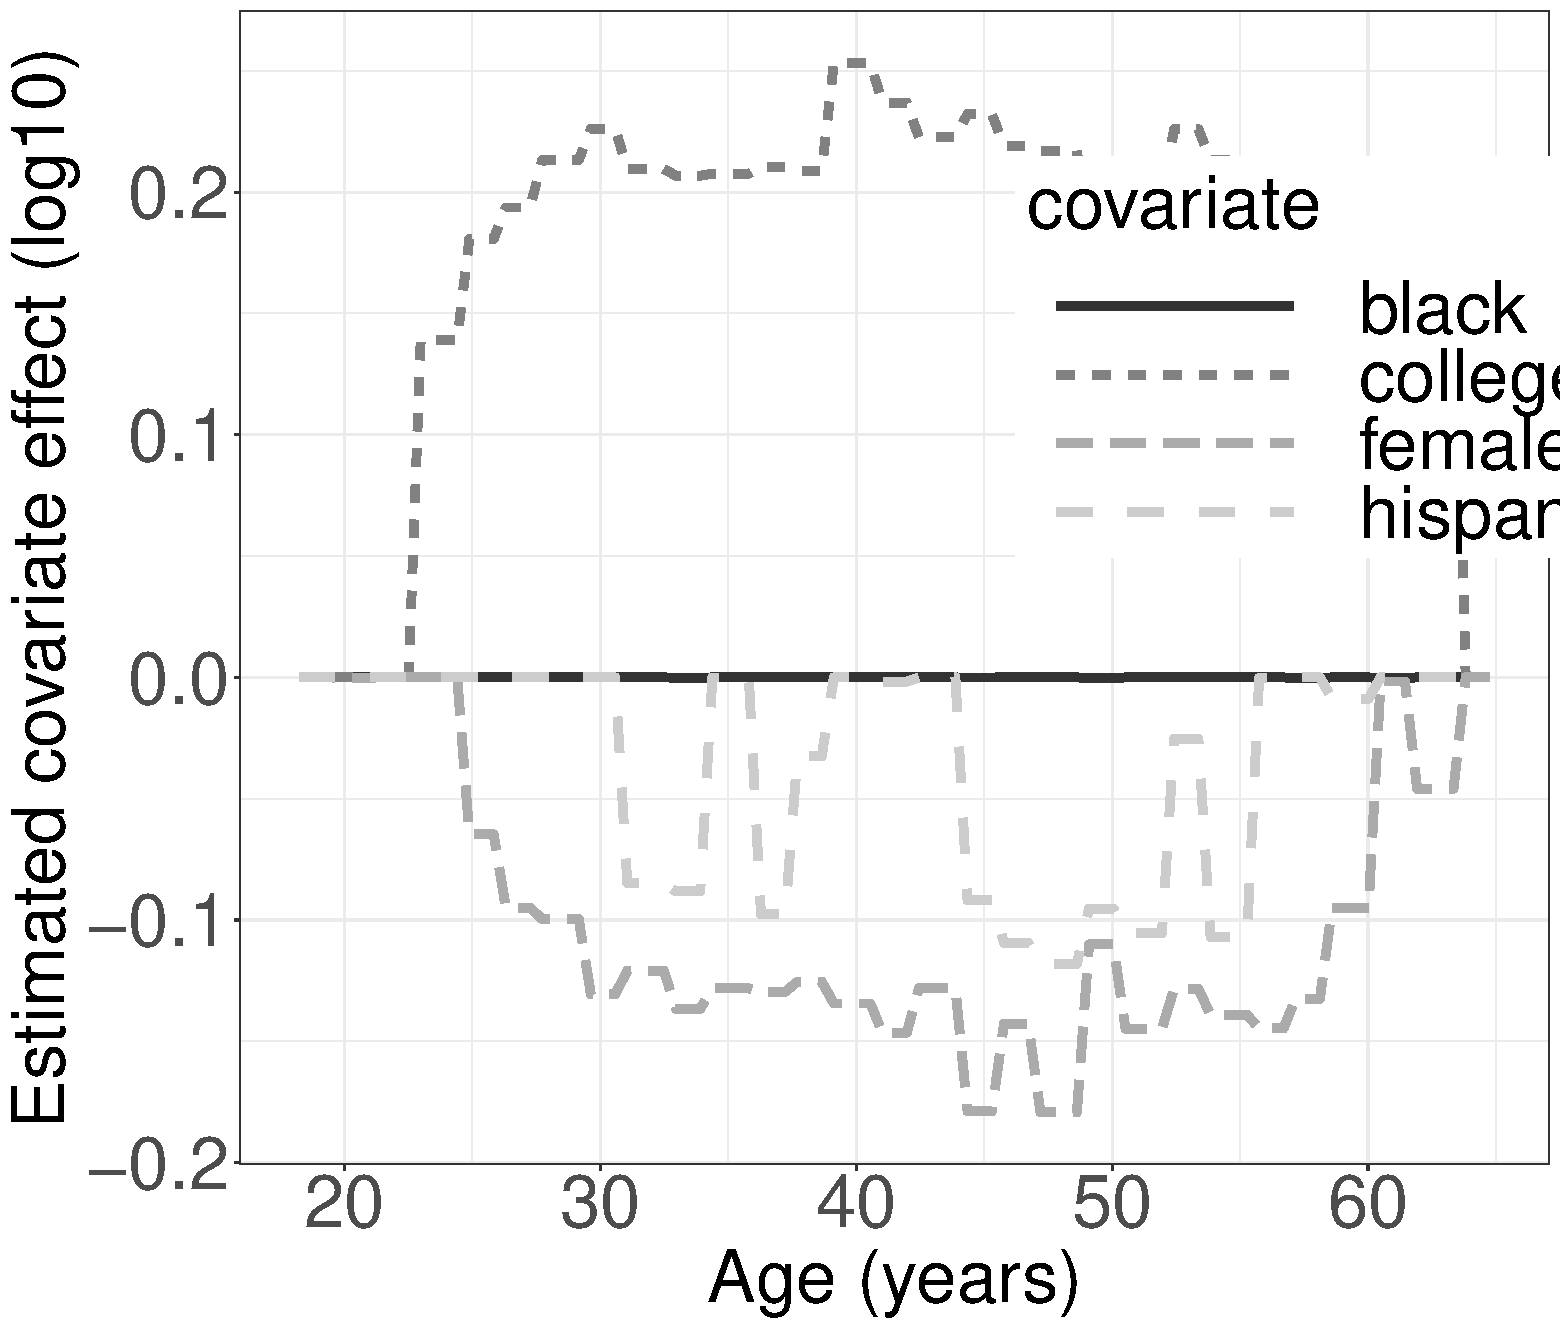
\includegraphics[width=0.5\textwidth]{figs/salary_estimated_effects_30knots.pdf}
\end{tabular}
\end{center}
\caption{Salary data results with fixed 20 (top) and 30 (bottom) fixed knots. 
Left: posterior probability of a salary gap associated with race, gender and college education versus age, adjusted by occupation and worker class. Right: corresponding estimated effect (log-10 scale)}
\label{fig:salary_suppl}
\end{figure}


The black race and female sex were found to be strongly associated to salary gap in our main analysis. To further explore this important source of potential salary discrimination, we repeated the analysis, now adding an interaction between black race and sex.
Figure \ref{fig:salary_female_race} shows that we obtained a small probability for the existence of said interaction, at all ages.


We also did additional analyses to assess the sensitivity of the results if one were to fix the number of knots, instead of using a multi-resolution analysis where one averages over resolutions.
Figure \ref{fig:salary_suppl} shows results for the salary data when fixing the number of knots to 20 (top panels) and 30 (bottom panels). The results suggest that, similar to what was observed in Figure \ref{fig:splinefit_suppl}, statistical power decreases when one adds more knots. This is apparent for covariates black and hispanic, which had the smaller estimated effects in our original analysis in Figure \ref{fig:salary} (where Bayesian model averaging was used to average over the uncertainty in the number of knots).
The results also suggest that there is no false positive inflation, covariates government and self-employed continue to show no local covariate effects at any age. Finally, covariates college and female are similar to our original analysis, in that they continue to be found to have a local effect on salary at almost all ages.



\subsection{Application to multi-electrode electrocorticography data}


\begin{figure}
	\begin{center}
		\begin{tabular}{cc}
		 	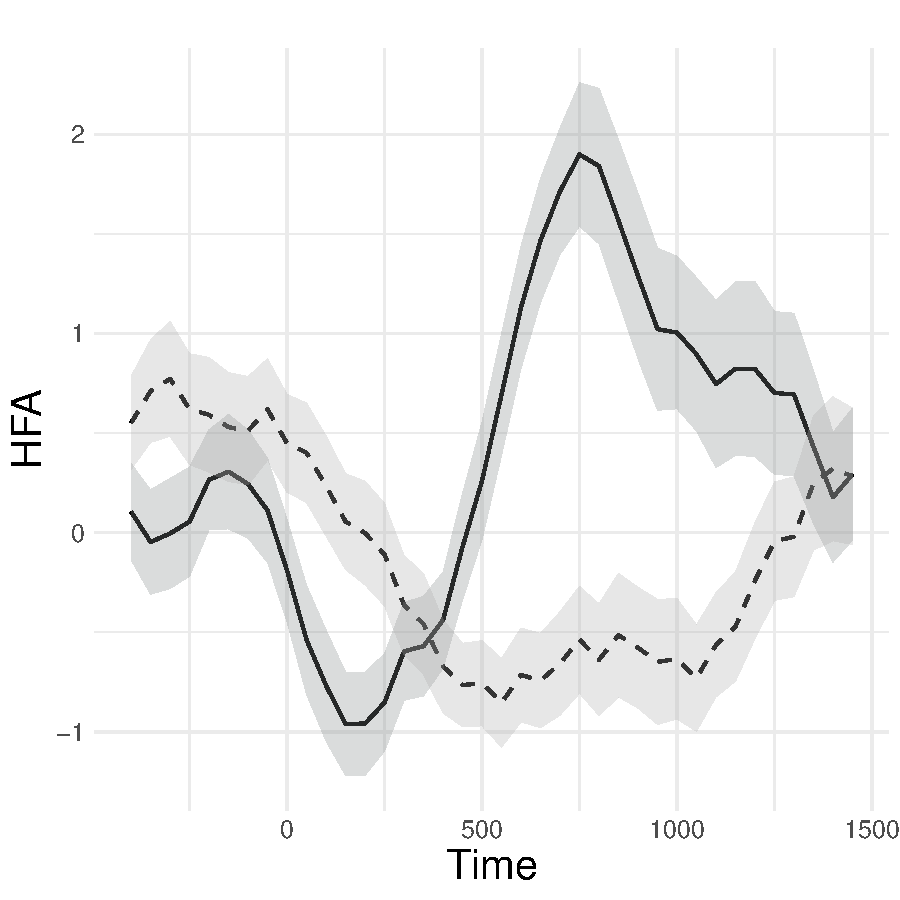
\includegraphics[width=0.45\textwidth]{figs/Ecog_trials1.pdf} &
			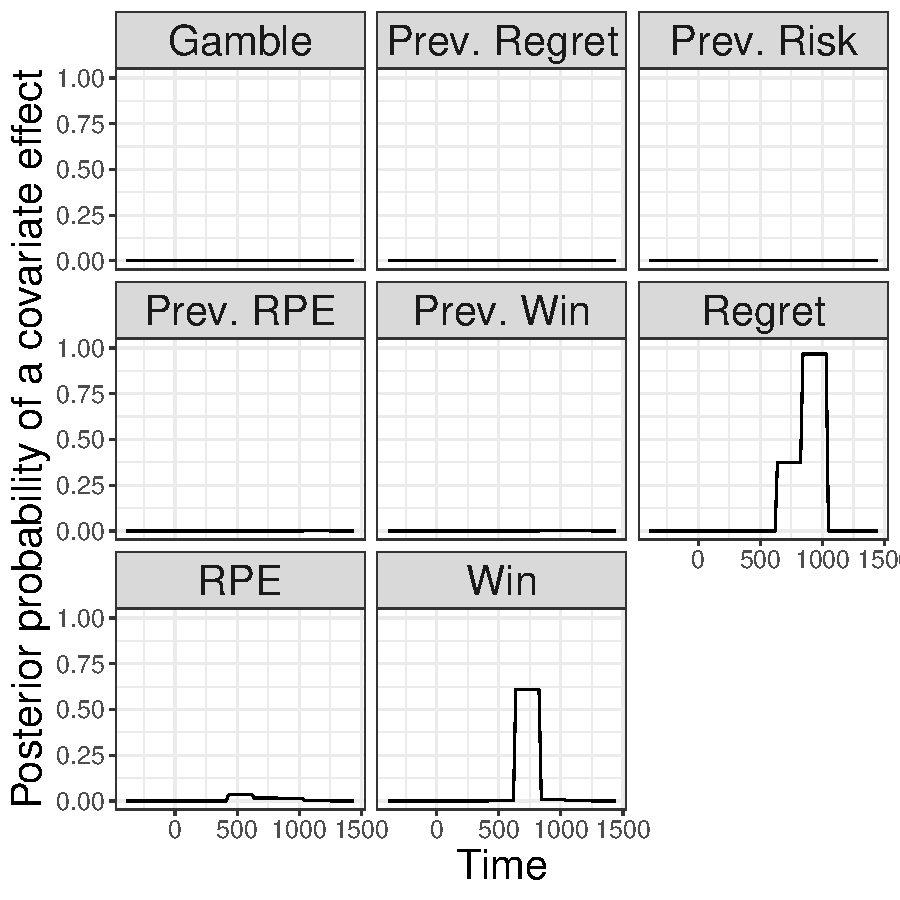
\includegraphics[width=0.5\textwidth]{figs/Ecog_pp_localtests_mr.pdf} 
		\end{tabular}
	\end{center}
	\caption{ECoG data. Left: mean high-frequency activity signal averaged across trials where the gamble was won (solid line) or lost  (dashed line), and point-wise 80\% confidence intervals. 
	Right: posterior probability of local covariate effects on brain activity}
	\label{fig:ECoG}
\end{figure}


\begin{figure}[htbp]
\begin{center}
\begin{tabular}{cc}
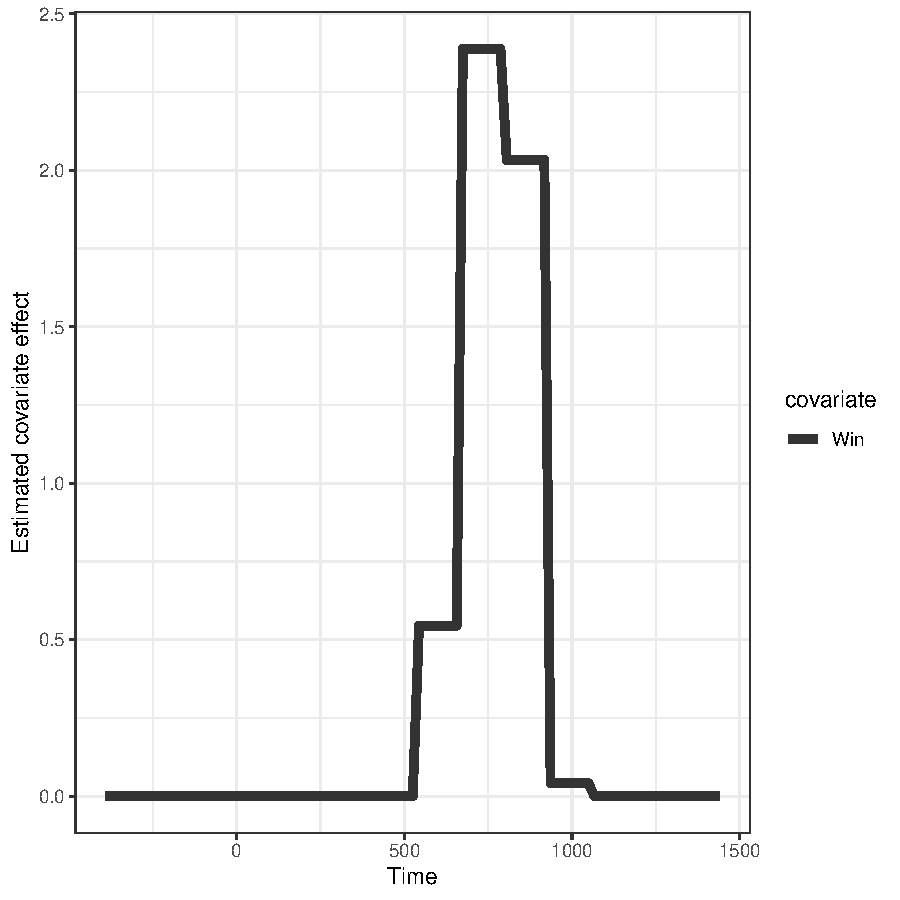
\includegraphics[width=0.45\textwidth]{figs/Ecog_estimate_fitwin.pdf} &
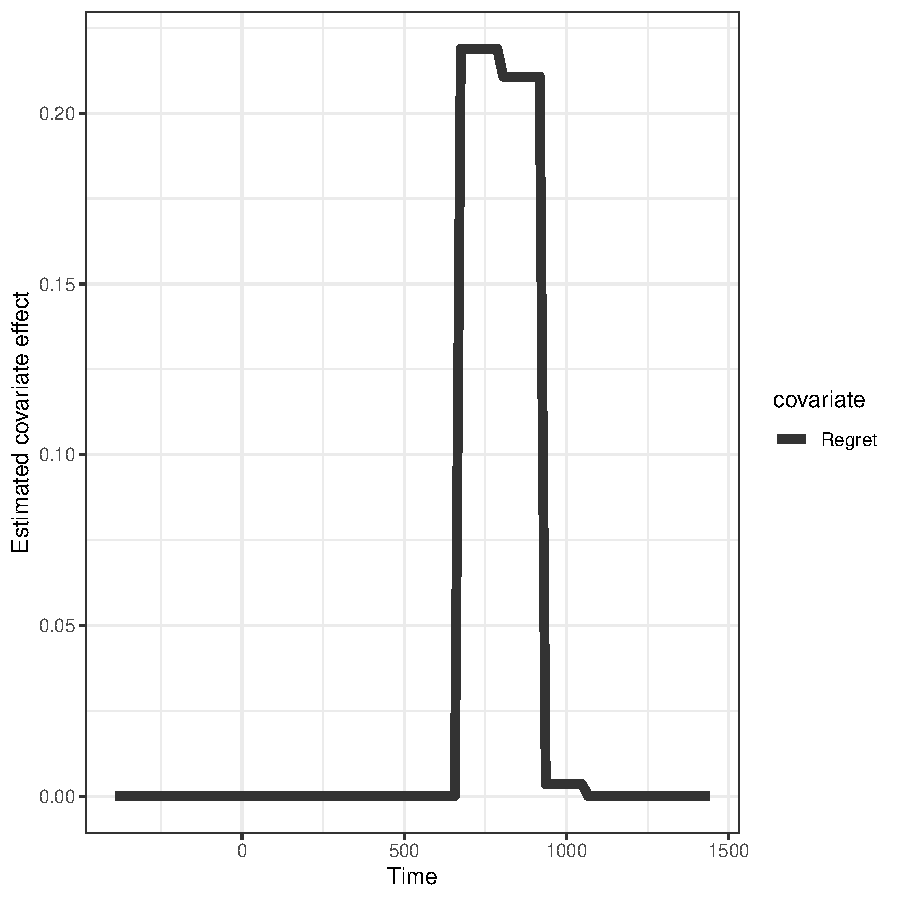
\includegraphics[width=0.45\textwidth]{figs/Ecog_estimate_fitregret.pdf} \\
Estimated effect of a Win/Loss over time &
Estimated effect of Regret over time \\
%
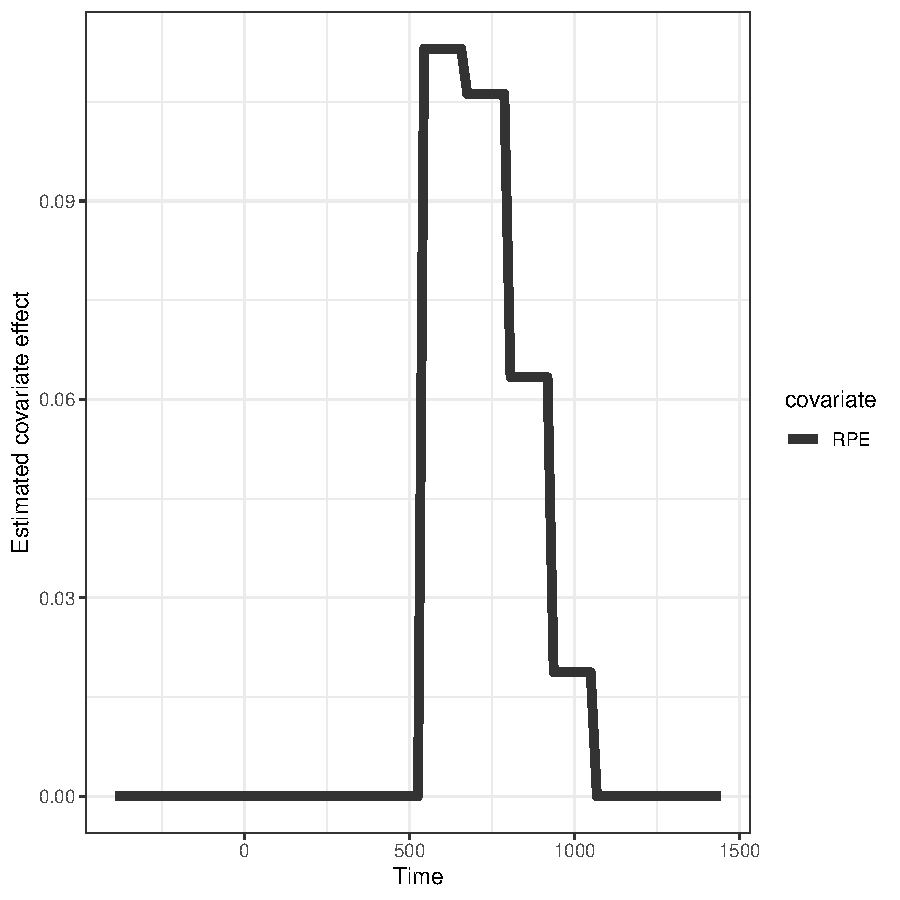
\includegraphics[width=0.45\textwidth]{figs/Ecog_estimate_fitrpe.pdf} &
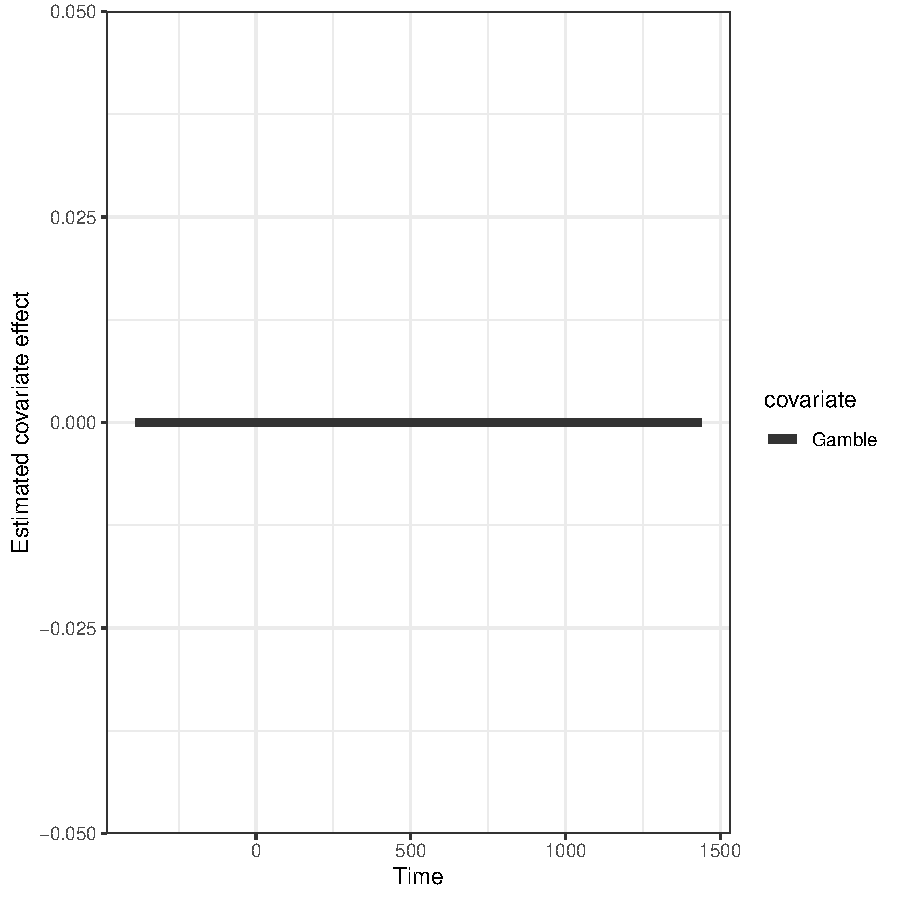
\includegraphics[width=0.45\textwidth]{figs/Ecog_estimate_fitgamble.pdf} \\
Estimated effect of the reward prediction error (RPE) over time &
Estimated effect of Gamble over time \\
\end{tabular}
\end{center}
\caption{Estimated time-varying effects of the three outcome-related covariates (Win, Regret, RPE) and the choice-related covariate Gamble in single-variate analyses for the application of Section \ref{ssec:saez_data}. Only Win and Regret show high posterior probabilities of having an effect on brain activity in the time intervals}
\label{fig:EcoG_effect_singles}
\end{figure}

\begin{figure}
	\begin{center}
		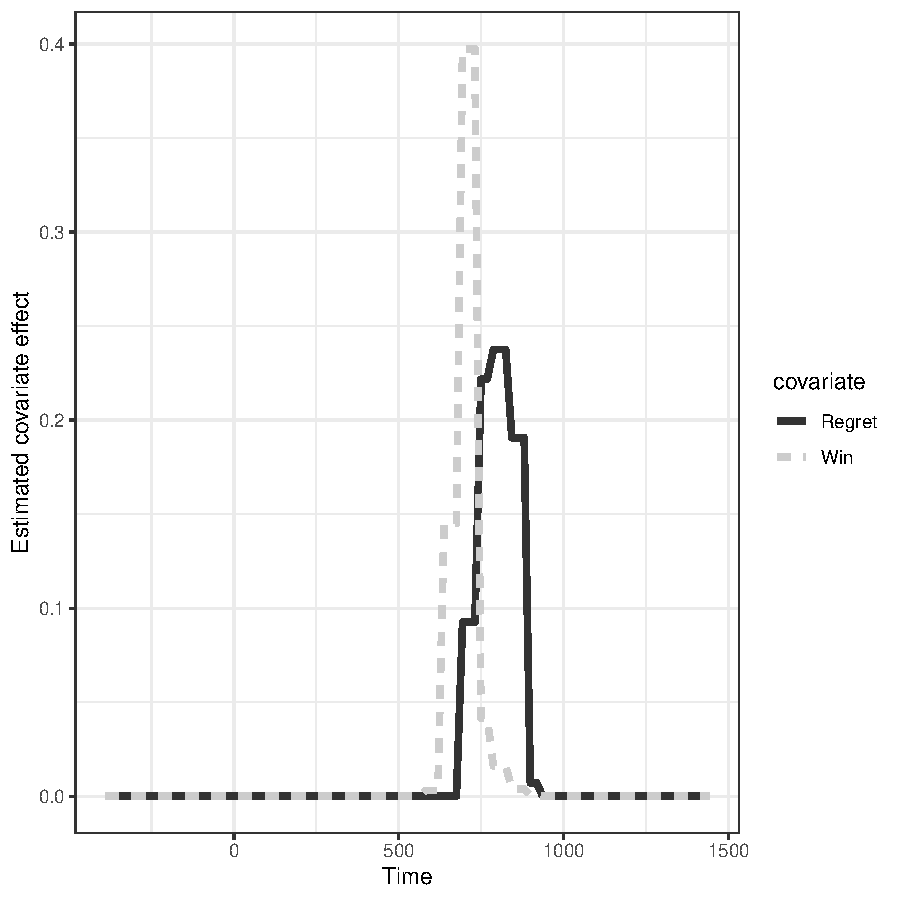
\includegraphics[width=0.7\textwidth]{figs//Ecog_estimate_fitmulti_mr.pdf}
	\end{center}
	\caption{Estimated time-varying effects of two outcome-related covariates (Win, Regret) in the multi-variable  analysis for the application of Section \ref{ssec:saez_data}.  The only relevant variable is Regret, with highest marginal probability of an effect $0.99$}
	\label{fig:EcoG_effect_multi}
\end{figure}





























% =============================================================================
\chapter{Supplementary Material for Chapter~3}
\label{chap:appendix3}
% =============================================================================

% [TODO: Derivation of the ELBO, additional simulation results, and
%  implementation details for the torch codebase.]

\section{ELBO Derivation}
\label{sec:app-ch3-elbo}

% [TODO: Full derivation of the evidence lower bound for the
%  variational objective in Section~\\ref{sec:ch2-inference}.]

\section{Additional Simulation Results}
\label{sec:app-ch3-sims}

% [TODO: Extended results across all simulation settings for Chapter 2.]

\addtocontents{toc}{\protect\setcounter{tocdepth}{2}}

%%% Local Variables: ***
%%% mode: latex ***
%%% TeX-master: "thesis.tex" ***
%%% End: ***
